\documentclass[letterpaper,12pt,oneside]{book}
\usepackage[top=1in, left=1in, right=1in, bottom=1in]{geometry}
%-----------------------__--------
%https://es.overleaf.com/project/642e50d937469ff17340bdc4
% Tesis UNAM https://tex.stackexchange.com/questions/234265/unam-thesis-title-page-portada-tesis-unam

\usepackage{chngcntr} % Paquete necesario para controlar contadores
\counterwithout{footnote}{chapter} % Evita que el contador se reinicie por capítulo

%\usepackage{parskip} % Add the parskip package


\usepackage{setspace} % Add the setspace package
\setstretch{1.5} % Set line spacing to double

\usepackage{pdfpages}
\usepackage{lipsum}

\usepackage[T1]{fontenc}
\usepackage[utf8]{inputenc}
\usepackage[spanish,es-nodecimaldot,es-tabla]{babel}

\usepackage{graphicx}
\usepackage{float}
\usepackage{tikz}
\usepackage{setspace}

%% para codigos
\usepackage{listings}


%Subfiguras
\usepackage{caption}
\usepackage{subcaption}

% Para referencias 
\usepackage{hyperref}
%%\usepackage{apacite}

\usepackage{url}

% Option B for bibliogaphy
\usepackage[backend=bibtex,style=ieee]{biblatex}
%\usepackage[backend=biber,style=apa]{biblatex}
\addbibresource{CARDIAC.bib}


%\addbibresource{CARDIAC}
%%% To make that images appear at the top of the page
	\makeatletter
	\setlength{\@fptop}{0pt}
	\makeatother
	%%%
\title{E-CARDIAC: La evolución hacia un modelo concurrente y paralelo}

\begin{document}
	\frontmatter
	\pagestyle{plain} % Set page style to "plain" for the front matter
	%\maketitle

    \includepdf{media/cover.pdf}

%---------------------------------
\chapter*{}
\begin{flushright}%
  \emph{``These are fast-moving times, and those who make no effort to understand computers may very well get left behind''}
  
  
  - David W. Hagelbarger, 1968
  %%\thispagestyle{empty}
\end{flushright}

\chapter*{Agradecimientos}
%\spacing{1.5}%\doublespacing

%%\chapter*{Abstract}

%% Palomita de revisado 2(completa)
\chapter{Introducción}

	Hoy en día tenemos multitud de aparatos electrónicos que suelen ser llamados computadoras; celulares, laptops, tabletas, relojes inteligentes y un sinfín más. 
	Estos aparatos suelen ser llamados así dado que son capaces de resolver operaciones aritméticas y lógicas, guardar datos, procesarlos y recibir instrucciones del 
	usuario; en otras palabras, de \textit{computar}. Esto, siguiendo la definición
	que recoge el diccionario de Oxford\footnote{Usado como fuente dado que la lengua franca de la computación es el inglés.}, tiene sentido,
	pero si analizamos más detalladamente el término ``computadora''  notaremos que el origen de la palabra es anterior a las computadoras
	tal cual las conocemos hoy en día.
	
	Por ejemplo, antes de 1950, la palabra ``computadora''  hacía referencia comúnmente a mujeres
	que trabajaban en la \textit{N.A.S.A.} y realizaban cálculos manuales. El blog \cite{nasa_who_2020} describe esta situación, dedicado a Katherine Johnson (destacada ``computadora humana''), nos muestra cómo aun con el machismo que se vivía en la época logró ser ampliamente reconocida, y vemos cómo esa misma palabra que la había descrito a ella en el pasado
	se empezó a usar para describir a las nuevas máquinas electrónicas de cálculo.

	Si viajamos al pasado remoto, notaremos que desde épocas muy tempranas se buscaba disminuir las tareas repetitivas para los humanos, pasando por el ábaco
	en muchas culturas, hasta máquinas más complejas a partir del siglo XVI, o con técnicas como los logaritmos y tablas de multiplicar. Esta búsqueda junto
	al desarrollo de otras tecnologías en paralelo permitió la creación de máquinas que podían ir más allá de automatizar cálculos,
	máquinas de propósito general, que pudieran cambiar su funcionamiento de acuerdo a la interacción con el usuario y resolver
	una multitud de problemas nunca antes pensados\cite{ifrah_universal_2001}. En tal estudio del pasado nos daremos cuenta de la cantidad de sucesos y desarrollos que tuvieron 
	que acontecer para llegar desde automatizaciones muy particulares de cálculos aritméticos, hasta las computadoras que conocemos hoy en día. 
	%Sinonimos?
	%%https://www.smithsonianmag.com/science-nature/history-human-computers-180972202/

	Aunque tenemos una remota idea de lo compleja que fue la invención de la computadora, no se suele conocer ni siquiera superficialmente
	la forma en que funciona una, el cómo podemos enviar mensajes de texto mientras escuchamos una canción, si acaso hay algún programa que ejecuta a los 
	demás programas que utilizamos, o incluso si hay un programa que da inicio a todos los procesos de una computadora. Al final, son temas complejos
	que requieren su tiempo de estudio. Lo que no puede suceder es que profesionales o estudiantes de carreras afines a la computación no conozcan estos detalles, y
	es que muchas veces se da por sentado que es conocimiento general, y en especializaciones como desarrollo web o arquitectura de \textit{software} (solo como ejemplo) no se le suele
	prestar mucha atención.
 
    Sin embargo, el conocimiento, al menos básico, del funcionamiento interno de una computadora es fundamental para saber
	cómo explotar de mejor manera los recursos de las máquinas que estás utilizando en cualquier disciplina en la que te desempeñes. Aunado a esto, conocer la historia
	es otro punto fundamental,
	ya que te permitirá saber la razón por la cual ciertos aspectos de las computadoras no han cambiado en 80 años y por qué otros han cambiado o evolucionado
	de manera tan vertiginosa en los últimos, preparándote también para el futuro y dando el reconocimiento que se merecen aquellas personas que,
	con sus aportes, contribuyeron a la revolución que trajo consigo la invención de la computadora.
	
	Estos pensamientos surgieron a lo largo de mi carrera universitaria, pero fue al final de esta que decidí abordarlos y empezar este proyecto de investigación,
	con el fin de centrar en un mismo texto un repaso histórico de la computación acompañado de una descripción didáctica del funcionamiento de las computadoras
	y su evolución a lo largo de la historia. Sin embargo, como la intención tampoco es crear un manual completo de las computadoras y su historia, el repaso
	se centrará principalmente en el origen de las computadoras y cómo funciona, \textit{grosso modo}, una computadora actual.
 
    Para esto último me apoyaré
	en \textit{CARDIAC (CARDboard Illustrative Aid to Computation)}, un modelo de computación 
	desarrollado por \textit{Bell Labs} de la mano de David W. Hagelbarger y Saul Fingerman en 1968 con la intención, precisamente,
	de hacer más fácil de entender a los alumnos de aquel entonces cómo funcionaba una computadora; el manual del modelo se puede consultar
	en \cite{fingerman_instruction_1968}. 
    Por supuesto, no fue el único modelo que existió, pero sí uno muy interesante para abordar
    los temas que he mencionado. Tanto este como otros
    modelos son mencionados en \cite{mark_jones_lorenzo_paper_2017}, que
	no puedo dejar de mencionar como una de las lecturas que más me inspiraron en la escritura de esta tesis.
	
	El reto con \textit{CARDIAC} es que, dado que fue creado en 1968, la concurrencia, el paralelismo o
	la inclusión de un sistema operativo no pasaban por la mente de sus creadores, puesto que aún no eran tan relevantes en la industria estos términos. Así que,
	para poder llegar a las computadoras actuales —concurrentes, paralelas, y con un sistema operativo—, decidí diseñar una ``evolución'' de CARDIAC que permita
	entender estos conceptos de una forma didáctica, aprovechando las ventajas que un modelo da al abstraer un sistema complejo en los componentes principales
	que se quieren dar a entender. Utilizando el contexto histórico se darán las razones por las que cada paso en la evolución de las
	computadoras fue necesario, e incluso a veces imparable, manteniendo la atención principalmente en estos tres conceptos.
	 
	Es claro que en todo este tiempo surgieron otros modelos con la intención de ayudar a los estudiantes a entender el funcionamiento de una computadora. Algunos
	de ellos que debo mencionar por su relación con CARDIAC son: \textit{MARIE (Machine Architecture that is Really Intuitive and Easy)}, un muy interesante 
	desarrollo presentado en \cite{null_essentials_2003}, que se enfoca en los aspectos básicos del funcionamiento al igual que CARDIAC; otro es un desarrollo
	hecho en Argentina alrededor de los años 80 llamado \textit{TIMBA (Terrible Imbecile Machine for Boring Algorithms)} que incluso tenía un lenguaje de programación,
	como nos describe el artículo \cite{alvaro_frias_retruco_2022} centrado en dicho lenguaje; por último, he de mencionar un desarrollo
	mostrado en el artículo \cite{ajdari_design_2012} que presenta a \textit{Abu-Reiah}, un procesador de 8 bits simplificado que incluye un simulador 
	gráfico
	para ayudar a los estudiantes de arquitectura de computadoras. Mi intención con las mejoras a CARDIAC no es suplir ninguno de los trabajos antes mencionados,
	sino más bien complementarlos con un desarrollo histórico que presente de forma clara, concisa y didáctica cuatro aspectos fundamentales en la evolución
	de la computación: la concurrencia, el paralelismo, el uso del sistema operativo, y la programación.
	
	
	Más allá del recorrido en la construcción y diseño de modelos ``evolucionados'' de CARDIAC, el texto se verá acompañado,
	tal como la clásica CARDIAC distribuida por \textit{Bell Labs}, con un ``kit'' que incluye un \textit{software} que contendrá tres máquinas virtuales\footnote{La simulación de una
	máquina física que virtualiza cada uno de sus componentes, incluido el \textit{hardware}.}. Será una para cada
	modelo de CARDIAC, con la diferencia de que estas máquinas virtuales ya no serán en papel, sino interfaces gráficas para uso en computadoras de escritorio con la idea de 
	que sea fácil para el estudiante
	entender la teoría y practicarla, así dando la posibilidad de que puedan experimentar en un ambiente controlado para poder ver cómo se van ejecutando los programas, lo cual en una versión paralela o concurrente sería un poco más difícil de ver con una 
	computadora de papel.

	

\tableofcontents
\listoffigures

\mainmatter

\chapter{Historia de la computación} 


	\section{Breve recorrido por el pasado}
		\subsection{Antecedentes}
		% máquinas parecidas a las computadoras, que no lo son
		
		Desde que los humanos empezamos a hacer cálculos, en el sentido de sumar o restar cantidades representadas por números, hemos necesitado de herramientas
		que nos apoyen en la resolución del cálculo. A medida que los cálculos se volvían más complejos, necesitábamos herramientas más complejas. 
		
		Las
		primeras herramientas para apoyarnos en esto fueron las representaciones de números de maneras abstractas, una evolución continua en la abstracción
		de los números permitió a algunas civilizaciones crear artefactos que nos permitieron aumentar nuestra capacidad de realizar cálculos
		, como el \textbf{ábaco}, el cual se ha encontrado
		en diversas civilizaciones en diferentes épocas de la humanidad. El más antiguo del que se tiene registro es el inventado por la civilización
		sumeria alrededor del año 2700 antes de nuestra era \cite{ifrah_universal_2001}.
  
        Otras civilizaciones siguieron sus desarrollos de manera independiente, no solo para llegar a un artefacto
		similar al ábaco, sino para evolucionar su forma de hacer cálculos y la complejidad de estos. Tal es el caso de los griegos, una de las civilizaciones
		más importantes de nuestro mundo, que dieron un gran aporte al desarrollo de la matemática, tanto que muchos de sus descubrimientos siguen siendo
		enseñados hoy en día; y que, por supuesto, aumentaron la complejidad en los cálculos aritméticos \cite{ifrah_universal_2001}.
  
        Esta evolución paralela entre la aritmética que teníamos como humanidad 
		y las herramientas para solucionar esos cálculos
		fue construyendo un camino, o quizá varios, que en ciertos puntos confluyeron en la creación del siguiente hito en la simplificación de la resolución
		de cálculos; la \textbf{calculadora}. De la misma forma, nos llevarían hasta la creación de la primera \textbf{computadora} digital, que posteriormente se convertiría
		en algo mucho más grande y completo de lo que quizá se imaginaba en su creación \cite{ifrah_universal_2001}.
		
		%% Ser más claro para la definición de lo que ingresa a la computadora
		Siguiendo la mencionada evolución, es importante destacar la época en la que surgieron las primeras calculadoras mecánicas, así
		como ciertas herramientas para minimizar el esfuerzo en los cálculos realizados por los usuarios. Es el siglo XVII en Europa occidental,
		saliendo del Renacimiento europeo, en el cual había necesidades más complejas en ciencias exactas y en problemas aplicados; los
		cálculos para la navegación y los astronómicos son ejemplos claros de ello. Por esa razón, el descubrimiento de
		los logaritmos por parte de John Napier, en 1614, fue uno de los grandes avances en la forma de resolver problemas aritméticos.
		Los logaritmos, \textit{grosso modo}, permiten sustituir multiplicaciones por sumas, lo cual implica una simplificación considerable
		en el tiempo de resolución de estas operaciones \cite[p. 24]{oregan_brief_2012}.
  
        Pero aun así, los cálculos seguían sin ser tan rápidos,
		por lo que se desarrollaron tablas de logaritmos, ya calculados, que acortaban el tiempo aún más. Otro avance relacionado fueron los dispositivos 	mecánicos que permitían optimizar algunos cálculos aritméticos. 
		\textit{The Gunter Scale} (la regla de Gunter) y \textit{The Slide Rule} (la regla de cálculo) fueron dos dispositivos que
		permitían al usuario conseguir tal optimización.
		La primera fue creada por Edmund Gunter y la segunda por William Oughtred como mejora a la primera. De hecho, \textit{The Slide Rule} siguió evolucionando a lo largo de los años para añadir más
		funcionalidades, incluido el uso de logaritmos, lo que la mantuvo vigente hasta hace relativamente poco tiempo (especialmente en áreas de ingeniería) \cite[p.24 y p. 96]{oregan_brief_2012}.		
 
  
		 Un poco más lejos llegarían Blaise Pascal y Wilhelm Gottfried Leibniz con sus inventos, que ya serían calculadoras en forma. Leibniz inventó la
		\textit{Step Reckoner}, o simplemente ``máquina de Leibniz'', en el año 1673, basándose en \textit{The Pascaline} (Pascal, 1642) ; 	
		ambas permitían hacer cálculos 
		aritméticos como la suma y la resta de manera mecánica \cite[p.25]{oregan_brief_2012}. 
		
		Aunque desde muchos años 
		antes se venía pensando
		en un dispositivo como la calculadora, la dificultad del proyecto había frenado su desarrollo. El mismo Leonardo da Vinci lo intentó, pero solo dejó sus planos para construir un dispositivo con esas características, puesto que no lo concretó. Ahora sabemos que el modelo de Leonardo sí era viable, solo que con tecnología más avanzada,
        dado que ingenieros de la época moderna pudieron seguir sus instrucciones para crear aquel dispositivo \cite{california_state_university_historical_nodate}.
  
		Podemos notar que las inquietudes por automatizar operaciones estaban
		ya desde antes que la tecnología, de su época, les permitiera a los inventores llevar a cabo sus planes. A pesar de esto, las siguientes
		generaciones seguían adelante con esas ideas, a veces directamente y otras de forma más independiente; demostrando que el avance
		teórico es completamente necesario, aunque no se tengan las herramientas en ese momento del tiempo para su desarrollo práctico. Este interesante patrón, donde la teoría avanza más rápido que los desarrollos prácticos, lo veremos de nuevo en 	
		repetidas ocasiones en el futuro.
		%Slide rule en ingenieria
		
		Aunque las máquinas de Leibniz y Pascal eran calculadoras en forma, su replicación no era sencilla y tampoco fueron realmente populares; pero
		si hay una época donde replicar máquinas para automatizar procesos va a estar en su auge, esa es la \textbf{Revolución Industrial}. En
		1820, un francés llamado Charles Xavier Thomas de Colmar construyó el \textit{Arithmometer}, basándose en la terminología de Leibniz, fue la primera
		calculadora en forma que se vendió masivamente. En los años sucesivos, continuó recibiendo mejoras y, al final, fue toda una inspiración para una multitud de inventores 
		en todo el mundo \cite[p. 127]{ifrah_universal_2001}.
		
		El antecesor directo de la computadora, y sucesor casi directo del ábaco, no solo había nacido, sino que ya había conseguido llegar a gran parte de
		la población. Así que, si ya se había logrado el reto, ¿cuál era el siguiente paso? ¿Hacerla más pequeña? Sí, más pequeña para que pudiera llegar a más personas,
		más veloz, y que pudiera hacerse más fácil el uso para el usuario; al menos esa sería la respuesta general. ¿Cuál sería la de un visionario? Alguien
		que piensa más allá de las convenciones quizá pensaría en un dispositivo que fuera capaz de alcanzar nuevos horizontes tecnológicos. 
  
        Esa persona era Charles 
		Babbage,
		un reconocido matemático de su época, miembro fundador de la \textit{Royal Astronomical Society} (1820), inventor y  pionero en la investigación
		de operaciones; alguien muy distinguido en su época, sin duda. Para el año de 1821, estaba diseñando su \textit{Differential Engine} (máquina diferencial), una máquina totalmente mecánica, que
		en principio buscaba resolver el problema de precisión que tenían las calculadoras del momento, además de resolver funciones polinómicas de hasta
		grado 6. Lamentablemente, no llegaría a ser producida por Charles, en parte por lo difícil (y costoso) que era en la época, y en parte porque Charles ya estaba pensando 
		en algo incluso más avanzado; aun así, la máquina se logró construir en 1853 por un par de ingenieros suecos que se basaron en los planes de Charles
		\cite[p.201]{oregan_brief_2012}.
		
		En lo que Charles ya estaba pensando, y en lo que se centró a partir de 1833, cuando se dio por terminada la construcción de la \textit{Differential Engine} (porque el maquinista que la 
		construía renunció), era en una máquina llamada  \textit{Analytical Engine} (máquina analítica), capaz de realizar cualquier tarea que pudiera
		ser expresada en notación algebraica,  y que disminuía la interacción humana para realizar los cálculos.   Era una máquina mucho más compleja; tendría un
		almacenamiento y un procesador al que Charles llamaba \textit{the mill} (el molino), porque tenía la forma de un molino y era la parte central que realizaba las operaciones. Además,
		contaría con elementos para la entrada y salida de datos usando la idea del \textit{telar de Jacquard}\footnote{Un telar inventado por el francés Joseph-Marie-Jacquard en 1804 para poder cambiar los patrones de los tejidos.}, que usaba tarjetas perforadas\footnote{Eran tarjetas de 
		cartón(usualmente) que tenían orificios con los que se representaban patrones, se continuaron usando por mucho tiempo en las computadoras digitales como podemos ver en 
		el vídeo: \emph{Punch Card Programming, \url{https://www.youtube.com/watch?v=KG2M4ttzBnY} }}
		para cambiar los patrones de diseños del telar \cite{oregan_brief_2012}.
  
        Charles pensó en usar estas tarjetas para representar números, que a su vez se pudieran utilizar para realizar las operaciones
		aritméticas de la máquina, y de esta forma,  que su máquina fuese ``programable''. Incluso consideraba dos tipos de tarjetas:
		
		\begin{enumerate}
			\item Tarjetas de operación
			\item Tarjetas de datos
		\end{enumerate}
		
		Con esta última idea, de hecho, se puede vislumbrar algo muy parecido a las computadoras con arquitectura von Neumann (que se analizarán más adelante): un procesador, almacenamiento interno y 
		programas almacenados (en forma de las tarjetas mencionadas) \cite[p.204]{oregan_brief_2012}. 
        Alguien que vio más una computadora, como la conocemos hoy en día, que una calculadora muy avanzada, como la percibía
        su propio creador, fue  Lady Ada Lovelace, una matemática
		que estaba entusiasmada con el trabajo de Charles y que era realmente brillante. En 1843, escribió un artículo que 
		nombraría \textit{Notes}, al final de una traducción  que realizó del francés al inglés de un trabajo
		 escrito por Luigi Menabrea sobre la \textit{máquina analítica}, el cual se puede consultar en \cite{lovelace_scientific_1843}. En este artículo, detalla el funcionamiento de la máquina, las cualidades que la 
		hacen diferente a las calculadoras de la época, y
		ejemplos de programas para cálculos realmente complejos, como el cálculo de los números de Bernoulli. De hecho, este último es considerado 
		por muchos como
		el primer programa de la historia \cite{eric_kim_ada_1999}.
  
        Por supuesto, tenía una cercanía muy alta con Charles, como se deja ver en su correspondencia, lo que le permitió llevar a cabo un 	
		trabajo muy completo. Esté artículo, junto con las notas de Ada, posteriormente sería publicado
		en la revista \textit{Scientific Memoir} bajo el título \textit{Sketch of the analytical engine invented by Charles Babbage}\cite{eric_kim_ada_1999}.
  
        Entre los elementos más valiosos que nos 
		dejó, se encuentran, por supuesto los programas y los detalles del funcionamiento de la máquina que realizó (junto a Menabrea), pero también su visión sobre el trabajo de 
		Charles, que era un tanto diferente a lo que él mismo consideraba. Ella pensaba que la máquina podría actuar sobre  algo más que números, si se creaban las relaciones correctas con los números,  como representación de algo 
		abstracto, podrían fungir como símbolos para resolver más tareas. Ada consideraba a la máquina analítica como algo muy lejano a las calculadoras de su época,
		y lo era en muchos sentidos, por lo que, aunque no fue construida en su tiempo, al igual que su predecesora\footnote{Fue construida en 1991 por un equipo en el museo de ciencia de Londres usando los planos de Charles, y es exhibida actualmente ahí, probando que Charles tenía razón.}, por sus aportes a la computación
		se le considera como la primera computadora(mecánica) de la historia\cite{eric_kim_ada_1999}. Podemos
  ver una representación de esta en la figura \ref{fig:analytical_engine}, donde también vemos a Ada y
  Charles trabajando con ella.
		
		\begin{figure}
		    \centering
		    \includegraphics[scale = 0.5]{media/Historia/analyticalEngine1_sydbeypadua.jpg}
		    \caption{The Analytical Engin. Fuente: Sydney Padua (2015)}
	    	\label{fig:analytical_engine}
		\end{figure}
				
		En los años siguientes el avance fue continuo con las máquinas calculadoras de propósito específico, por ejemplo, Herman Hollerith,
		el fundador de la empresa hoy conocida como IBM,
		desarrolló una máquina de censos que usaba el concepto de las tarjetas perforadas para
        contabilizar datos. También la tecnología en general evolucionó:
		la era de la electricidad y lo electromecánico llegó a finales del siglo XIX, cambiando por completo las cosas. Junto al invento del tubo de vacío y avances teóricos como el álgebra de Boole, entre otros, fueron parte fundamental de las continuas invenciones del siglo XX \cite[p. 127]{ifrah_universal_2001}.
  
        Me parece importante destacar que no es una sucesión lineal de hechos o descubrimientos
		lo que llevó a la creación de la computadora digital, o de sus predecesoras, sino que el avance en muchas ramas de la ciencia, de la mecánica y otras
		disciplinas fue lo que condujo al descubrimiento de nuevas tecnologías a partir de la unión de todas estas áreas de estudio. En la siguiente sección analizaremos, principalmente, ese avance teórico que dio lugar a la evolución de las ``calculadoras'' mecánicas.
		
		% Usar automatas está bien?

			
		% Palomita de revisado
		\subsection{Primeros autómatas}
		% Breve historia de como se fue desarrollando la computación desde los inicios hasta llegar a automatas(1950)
		
		Los avances tecnológicos en las máquinas que automatizan cálculos no pararon, e incluso mejoraron en el siglo XX con la llegada de la electricidad
		y la electromecánica. Para el año 1913, el matemático español Leonardo Torres Quevedo desarrolló su \textit{Aritmómetro electromecánico}, evitando las
		dificultades que había tenido Babbage gracias a la electromecánica, le fue posible culminar este desarrollo que resolvía diversos
		problemas aritméticos. Este invento, además, incluía una máquina de escribir como entrada \cite{museo_torres_quevedo_ajedrecista_nodate,ifrah_universal_2001}.
  
        Este no sería el único aporte de Quevedo
		a la computación, otro de los hechos por los que es conocido es por sentar las bases de la \textit{automática} en su \textit{Ensayo sobre automática}.
		Tomando
		la definición de autómata como ``máquina que imita la figura y los movimientos de un ser animado'', Quevedo desarrolló la idea centrada en las posibilidades
		de las máquinas como calculadoras, pero que pudieran reconocer más objetos, más situaciones y resolver problemas más difíciles, para así
		quitarles trabajos repetitivos a los humanos. Él, en su afán de demostrar que su teoría tenía sentido, desarrollo un autómata llamado
		\textit{El Ajedrecista}, que en su primera versión podía terminar un juego de ajedrez, es decir, no podía jugar la partida completa,
		pero sí podía terminarla \cite{museo_torres_quevedo_ajedrecista_nodate,ifrah_universal_2001}.
		% Cambiar citas para incluir el ensayo de Leonardo Torres Quevedo
		
		Quevedo había lanzado preguntas muy interesantes en su ensayo acerca de los autómatas que se relacionan directamente con la computación, pues cuestiona
		las capacidades de una máquina para hacer algo más que lo que se lograba con una calculadora. Motivados por \textit{los problemas
		de Hilbert}, una serie de problemas matemáticos que buscaban dar más rigurosidad a las matemáticas desde el principio del siglo XX, Alan Turing
		y Alonzo Church continuaron ese camino al comenzar a trabajar, por separado, en resolver un problema muy particular: el famoso \textit{problema de la parada} \cite{ifrah_universal_2001}. 
  
        Sin entrar en mucho
		detalle, el problema de la parada trata sobre la posibilidad de determinar, dado un algoritmo y una entrada, si la ejecución de ese algoritmo se 	
		detendrá en algún momento o continuará indefinidamente. Si un algoritmo se detiene, proporciona una solución; si no, no podemos asegurar que el 
		problema tenga una respuesta computable. La respuesta al problema de la parada es compleja y no es
		la intención de este texto entrar en esos detalles, pero es importante comentarlo por lo fundamental que fue para entender los 
		límites de la computación \cite{ifrah_universal_2001}.
		
		Turing desarrolló modelos teóricos de máquinas que podían ``computar'' en el sentido más clásico de la palabra, es decir, hacer cálculos para resolver 
		problemas. Dentro de su amplio trabajo, Turing trató de crear
		una máquina lo más general posible, de forma que cualquier problema se pudiera computar en esa ``máquina de propósito general''; a tal máquina la llamó \textit{Máquina Universal de Turing} en su famoso artículo
		\textit{On Computable Numbers, With an Application to the
		Entscheidungsproblem}\footnote{En 1936 se presenta la tesis de Alan Turing y Alonzo Church, con
		aproximaciones distintas a la solución del problema de la parada.} (Sobre números computables, con aplicación al problema de la parada)\cite{ifrah_universal_2001}.
  
        Un modelo
		totalmente teórico, pero que mostraba todo el potencial de una máquina de propósito general que podía resolver cualquier problema que pudiese ser 
		expresado
		como un algoritmo. Sin embargo, Turing demostró que existen límites fundamentales en lo que se puede computar. En particular, el problema de la parada	
		muestra que no existe un algoritmo general que pueda determinar si cualquier programa se detendrá o no. Esto implica que no todos los problemas 		
		matemáticos son decidibles, es decir, no existe un algoritmo que pueda resolverlos todos. Así, la respuesta al problema de la parada es negativa: no 
		se puede determinar de manera general si un algoritmo dado se detendrá o no \cite{ifrah_universal_2001}.
  
        De esta forma, se iba creando lo que posteriormente sería conocido como \textbf{teoría de la computación}, un estudio  matemáticamente riguroso
		sobre las capacidades de las máquinas de cómputo. Esta se subdivide en varias ramas, una particularmente interesante es la \textit{teoría de la computabilidad}. Esta teoría estudia
		cuáles algoritmos puede computar una máquina para llegar a establecer si ciertos problemas son \textit{no computables} y, por ende, no son solubles por medio de ninguna computadora \cite[p. 272]{ifrah_universal_2001}.
		
		La forma de pensar sobre las máquinas ha evolucionado mucho a este punto en la historia; la visión ahora es sobre una máquina que dé soluciones a problemas que
		puedan ser descritos en forma de algoritmo, y ya no solo soluciones a problemas aritméticos o de funciones matemáticas. Turing y Church
		son dos nombres fundamentales en esta ciencia, que en ese momento aún no existía, de la teoría de la computación. En esos mismos años, la evolución
		de las máquinas continuaba, y en los siguientes años su expansión, causada también por el conflicto armado
		de la Segunda Guerra Mundial, no haría más que acelerarse.
		
		\clearpage		
		%% Palomita de revisado
		\subsection{Primeras computadoras}
		%1930-1945
		
		Es el momento de hablar de computadoras en forma, máquinas que ya se pueden considerar uniformemente como computadoras según la definición general
		que se tiene de estas. Repasaremos lo sucedido entre 1930 y 1946, cuando por diversas causas, la madurez en el entendimiento de las
		máquinas de cálculo, de la electromecánica y de la electricidad, así como la necesidad de una mejora tecnológica para enfrentar una de las guerras
		más crueles que ha visto la humanidad, se dieron las condiciones para el desarrollo de la computación. En primera instancia
		como la evolución de calculadoras, pero que se fueron transformando hasta convertirse en máquinas que resolvían problemas más allá de 
		la aritmética.
		
		Como en esta parte de la historia se centrada la discusión de cuál fue la primera computadora de la historia, es necesario tener una definición
		más clara de lo que entendemos por computadora, porque ciertas máquinas están en el limbo entre ser calculadoras o computadoras, mientras que otras ya son computadoras en un sentido más completo. Empecemos con la definición 
		del diccionario de Oxford, que uso dado que es entre Gran Bretaña y Estados Unidos donde se da principalmente el desarrollo de las computadoras
		en sus inicios, por lo tanto, es su \textit{lingua franca}:
		\begin{enumerate}
			  \item[] \emph{ Definición 1:} Una persona que hace cálculos, especialmente con una máquina de calcular.
			  \item[] \emph{ Definición 2:} Un dispositivo electrónico para guardar y procesar datos, típicamente en forma binaria, de acuerdo a las instrucciones
			  dadas en un programa(conjunto de instrucciones).
		\end{enumerate}
		
		La primera definición, que aún perdura, hace referencia principalmente al significado que tenía antes de 1940. Posteriormente, entre 1940 y 1950,
		con la aparición de las máquinas electromecánicas, se empezó a usar el término con la connotación que tenemos de él hoy en día. Por ende,
		la segunda definición nos interesa más.  Profundizando en la idea de la segunda definición, en \cite{goldstine_computer_1972} Goldstine nos dice lo siguiente 
		acerca de la computadora: ``Es un dispositivo electrónico que puede recibir un conjunto de instrucciones, o un programa,
		y entonces resolver este programa realizando varias operaciones matemáticas en datos numéricos.'' A partir de estas definiciones podemos establecer
		cuatro características fundamentales en una computadora:
		
		\begin{enumerate}
			\item Es un dispositivo electrónico. 
			\item Es capaz de almacenar datos.
			\item Es capaz de procesar datos.
			\item Realiza operaciones a partir de un conjunto de instrucciones dadas por el usuario, entendiendo conjunto de instrucciones/programa como una forma de algoritmo.
		\end{enumerate}
		
		Podemos notar fácilmente que un dispositivo de este estilo se ajsuta a nuestra comprensión de lo que es una computadora. Pero hay un punto 
		importante para nuestro 
		estudio, ¿que no sea un dispositivo electrónico es
		suficiente para que una máquina que tiene las otras tres características se deje de considerar como computadora? La mayoría de los autores lo manejan directamente
		como un dispositivo electrónico y no se involucran en una discusión más profunda del tema. Como veremos, realmente un dispositivo mecánico o electromecánico
		puede cumplir con el resto de especificaciones, pero dado que su uso se ha limitado a los inicios de la computación, y que quedaron rápidamente sobrepasados por la potencia de los dispositivos electrónicos, la definición tradicional de computadora se quedó únicamente con estos últimos.
		
		%% Pre - Guerra
		%Palomita de revisado
        \subsubsection{Época previa a la Segunda Guerra Mundial}
		
		En esta época, hubo una gran explosión de desarrollos en cuanto a máquinas que automatizaban cálculos; desde
		aquellas que eran calculadoras muy potentes, algunas que ya entran en la discusión de si son o no computadoras, hasta las que evidentemente lo son. Un ejemplo a 
		resaltar es la \textit{Differential Analyser}, creada por Vannevar Bush en 1931 en el M.I.T., uno de los logros más representativos en la historia de las calculadoras
		análogas\footnote{La mayoría de las máquinas actuales son digitales debido a su operación sobre cantidades discretas, mientras que los equipos análogos operan
		sobre cantidades continuas, que en versatilidad han quedado superados por las máquinas digitales.}. Esta máquina podía resolver una mayor 
		variedad de ecuaciones, lo que la convirtió en la primera calculadora análoga multipropósito \cite[p.158]{ifrah_universal_2001}.
  
		Otra calculadora realmente llamativa de ese momento fue la \textit{Complex Number Calculator}, creada por		
		Samuel Williams y George Stibitz en los laboratorios Bell en 1939, una calculadora electromecánica capaz
		de manejar números complejos. Esta contribución no fue única por parte de Stibitz, ya que en Bell Labs desarrolló muchos conceptos relacionados con la
		comunicación y la computación, generando así una de las etapas más brillantes para Bell Labs \cite[p.207]{ifrah_universal_2001}.
		
		
		Precisamente, entre estos dos sucesos, el alemán Konrad
		Zuse estaba trabajando en la construcción de prototipos de máquinas que disminuyeran su trabajo como ingeniero. Para 1938, había desarrollada la \textit{Z1:}
		una calculadora binaria, mecánica, de accionamiento electromecánico, que leía instrucciones de una tarjeta perforada. Para 1939, Konrad llevaría más lejos esta idea,
		eliminando la dependencia de las partes mecánicas, que eran muy complejas, y sustituyéndolas por relés para funcionar con circuitos eléctricos y
		puertas lógicas (\textit{AND, OR, NOT}). Esto lo logró aprovechando las ideas de Claude Shannon, quien introdujo la idea de implementar
		el álgebra booleana mediante relés eléctricos para crear circuitos; y así lo hizo Konrad en su \textit{Z2} \cite[p.206]{ifrah_universal_2001}.
  
		Su siguiente gran trabajo no tardó en llegar, y es por el que es recordado principalmente: la \textbf{Z3} (se puede ver en la figura \ref{fig:zuse_z3}), máquina que fue terminada en 1941. Usaba 2,600 relés, realizaba aritmética de punto flotante, tenía una 'longitud de palabra'\footnote{En esos años se usaba esa expresión para referirse al tamaño de una variable.} de 22 bits, contaba con un almacenamiento de 64 palabras, y los cálculos eran realizados puramente en binario dado que Zuse lo consideraba más eficiente. Era programable mediante tarjetas
		perforadas y completamente automática, hoy en día es considerada por ciertos autores, incluido G. O'Regan \cite{oregan_brief_2012}, como la primera computadora de programas almacenados de la historia.
  
		
		Lamentablemente, resultó destruida en 1943 por un bombardeo, y aunque fue posteriormente reconstruida para demostrar sus capacidades, en su momento fue un impedimento para afirmar que fue la primera computadora. De hecho, la Z3 es más parecida a las computadoras actuales que a otras de más renombre, como
		la \textit{ENIAC}. Incluso, en 1998, Raúl Rojas probó que la Z3 es \textit{Turing completa}, lo que demuestra que era
		una computadora con la capacidad de computar cualquier problema que pudiera ser expresado como un algoritmo 
		\cite{wikipedia_z3_2025,rojas_r_ieee_annals}.
  
        A pesar de los problemas en Alemania, Zuse pudo construir
		una versión más avanzada, a la cual llamó \textit{Z4}, que fue la primera computadora comercial del mundo, introducida al mercado en 1950. Aunque el desconocimiento
		sobre Konrad en el resto del mundo fue alto, en los últimos años, los museos y los autores le han dado el lugar que merece como uno de los padres de la computación \cite[p.206]{ifrah_universal_2001}.
		
		\begin{figure}
		    \centering
		    \includegraphics[width=0.7\textwidth]{media/Historia/CHM_computers_1941.zusez3.jpg}
		    \caption{The Zuse Z3 Computer. Fuente: Computer History Museum}
	    	\label{fig:zuse_z3}
		\end{figure}
		
		
		
		% Palomita de revisado
        \subsubsection{Época de la Segunda Guerra Mundial}
		
		La discusión sobre quién construyó la primera computadora fue un tema de controversia, tanto que se llevó a tribunales en Estados Unidos. Esto se debió a que los creadores
		de la computadora llamada \textit{ABC} afirmaban que John Mauchly, co-creador de \textit{ENIAC}, había visto previamente a la ABC. Finalmente, el dictamen estableció
		que el concepto de la computadora fue la concepción de diversas ideas por muchas personas, por lo que no era patentable. Una resolución que tiene mucho sentido
		dada la historia que hemos revisado sobre la creación de las computadoras, ya que muchas mentes han aportado en diversos aspectos a la concepción de lo que hoy
		en día conocemos como computadoras \cite{computer_history_museum_computers_nodate}.
		
		
		Justamente, veamos a uno de los implicados en la disputa, que siguió al desarrollo de Zuse, pero sin relación con él. La computadora fue nombrada como 
		\textit{The Atanasoff-Berry Computer (ABC)}, construida por el profesor John Vincent Atanasoff 
		en el Colegio Estatal de Iowa con la ayuda de su estudiante Clifford Berry entre 1939 y 1942. Tenía un sistema binario para la aritmética, memoria
		para guardar datos, circuitos electrónicos y separación entre datos y programas; era, en toda regla, una computadora, aunque no programable y de propósito
		específico \cite[pp. 212-218]{ifrah_universal_2001}.
  
        Otro desarrollo en paralelo, pero
		esta vez en el M.I.T., fue la \textit{Harvard Mark I}. Fue construida por Howard Aiken y un equipo con el apoyo de IBM, destinada a ayudar con cálculos balísticos
		en la Segunda Guerra Mundial; una máquina electromecánica que fue la primera en ser capaz de imprimir tablas matemáticas, algo que Babbage soñó casi un
		siglo atrás \cite[pp. 212-218]{ifrah_universal_2001}.
  
        Algo interesante a destacar de esta máquina es que no tenía las instrucciones y los datos guardados en la misma 
		``memoria'', a diferencia de las que hemos
		visto y lo que será el estándar en cuanto a arquitectura de computadoras. A este tipo de arquitectura se le llamará
		arquitectura Harvard con la llegada de los microprocesadores, una arquitectura que hoy en día es cada vez más relevante, pero que en su momento
		no fue la arquitectura central del desarrollo de las computadoras \cite{pawson_myth_2022}.
		
		%% No leí el articulo completo, solo el preprint	
		
		%%Tres?
		Después de revisar algunas computadoras un tanto desconocidas, nos quedan dos que son quizá las más famosas de la época. Empezando con la 
		\textit{Colossus Mark 1} (figura \ref{fig:colossus}), uno de los grandes aportes que dejó \textit{Bletchley Park}\footnote{Es el nombre de una instalación militar localizada en Buckinghamshire, 	Inglaterra.}, instalación especializada en el trabajo de descifrado de códigos durante la Segunda Guerra Mundial. Con una máquina de descifrado llamada \textit{Bombe}
		lograron desencriptar los mensajes de la famosa máquina \textit{enigma}, pero con el avance de la guerra se encontraron con un problema aún mayor: la máquina
		\textit{Lorenz SZ40/42}, que tenía una codificación de muy alta calidad y se usaba únicamente para los mensajes más importantes en la armada alemana \cite{oregan_brief_2012}.
  
        Para
		descifrar estos códigos entra en escena Tommy Flowers, diseñando la \textit{Colossus Mark 1}, una máquina semiprogramable que usaba tubos de vacío, lo que la hacía
		relativamente veloz para la época, logrando realizar
		una cantidad ingente de cálculos matemáticos con el fin de descifrar los mensajes que usaban la codificación Lorenz; estuvo disponible a principios de 1944, y
		su segunda versión se lanzó unos meses después. Dado su uso militar, su existencia se mantuvo
		en alto secreto por orden del gobierno hasta los años 70, hoy en día, se conserva una réplica de la máquina en el museo de Bletchley Park  
		\cite[p.39]{oregan_brief_2012}.
		
		\begin{figure}
		    \centering
		    \includegraphics[width=0.7\textwidth]{media/Historia/CHM_computers_1944.colossus.jpg}
		    \caption{Colossus Mark 1. Fuente: Computer History Museum}
	    	\label{fig:colossus}
		\end{figure}
		
		Prácticamente en paralelo, se estaba desarrollando
		en Estados Unidos una computadora electrónica digital con propósitos militares, centrada en realizar cálculos de artillería para el gobierno,
		\textit{ENIAC (Electronic Numerical Integrator and Computer)}; computadora construida por John Mauchly, J. Presper Eckert, y un equipo en
		el que se encontraba como consejero externo John von Neumann, en
		\textit{The Moore School of Electrical Engineering} de la Universidad de Pensilvania. Esta computadora, a pesar de ser de propósito específico,
		al ser programable, se le considera una de las primeras computadoras de propósito general \cite{ifrah_universal_2001}. 
  
        Su programación era muy compleja, ya que requería de mover o reordenar
		interruptores manualmente e ingresar la información por medio de tarjetas perforadas, 
		lo cual era realmente tedioso y tomaba demasiado tiempo. Además, si le sumamos que  los tubos de vacío que usaba no eran muy confiables, puesto que 
		estos explotaban 	
		fácilmente, tenemos una máquina que no era muy confiable y  bastante lenta de programar. A pesar de que no se termino antes de finalizar la 
		guerra (Segunda Guerra Mundial), pues fue puesta en ejecución hasta diciembre de 1945, fue utilizada en los años 
		porteriores por el gobierno estadounidense \cite{ifrah_universal_2001}.
		
		%% Post- Guerra, palomita de revisado
        \subsubsection{Época posterior a la Segunda Guerra Mundial}
		
		Fue precisamente en la Segunda Guerra Mundial donde se dieron algunos de los avances más importantes en la historia de la computación, donde se cambió la forma de
		concebir las computadoras, pasando de pensar en ellas como máquinas que solo resolvían cálculos aritméticos simples, a máquinas que resuelven problemas más avanzados, descifran
		códigos, calculan trayectorias para
		misiles, y demás tareas propias de una guerra. La necesidad del avance tecnológico llevó a estos desarrollos a su cúspide, pero con el final de
		la guerra los desarrollos no pararon, sino que se incrementaron, y la idea de una computadora de propósito general se veía
		presente en las mentes de los científicos que habían impulsado, y seguían impulsando, los desarrollos de máquinas cada vez más potentes.
		

		En 1946, con la Segunda Guerra Mundial terminada, Arthur Burks, Herman Goldstine y John von Neumann 
		escriben
		un  ensayo llamado \textit{Preliminary Discussion of the Logical Design of an Electronic Computing Instrument} (discusión preliminar de la lógica en el diseño de un instrumento electrónico de computación), para sintetizar las ideas que existían sobre estos dispositivos electrónicos, obtener una imagen de la situación en la que estaban y
		presentar cómo los problemas matemáticos podían ser ahora codificados en un lenguaje que la máquina entendiera \cite{randell_preliminary_1982}. Es en este documento donde
		se establece por primera vez la arquitectura de una computadora con  \textit{programas almacenados}, un concepto fundamental que, hasta hoy
		en día, la mayor parte de las computadoras utiliza.
  
        Notaremos que en el título de su ensayo no usan en ningún momento la palabra 'computadora', y
		es que para ese moemento no era un termino común. Como hemos venido leyendo, el uso generalizado de la palabra computadora
		se daría durante el mismo desarrollo de estos dispositivos.
  
        Von Neuman es alguien que aportó mucho a la computación. Poco antes, ya había escrito un reporte llamado \textit{First Draft of a Report on the EDVAC} (Primer borrador de un reporte sobre \textit{EDVAC}),
		puesto que se había unido a Eckert y Mauchly en el desarrollo de
		\textit{EDVAC (Electronic Discrete Variable Automatic Calculator)}. En tal reporte se detalla el diseño de un sistema de computación digital, automático
		y de alta velocidad. Fue uno de los textos que marcaron la época y sirvió de inspiración a otros, uno de ellos fue Maurice Wilkes, quien desarrolló su propia
		computadora con programas almacenados, la \textit{EDSAC (Electronic Delay Storage Automatic Computer)} \cite{oregan_brief_2012}. 
  
        La construcción de la \textit{EDVAC} tenía la intención de mejorar en los aspectos donde la \textit{ENIAC} fallaba.
		Un punto fundamental es que estaba construida con una arquitectura de programas almacenados, es decir, que no se necesitaba reconectar 
		cables para
		poder ejecutar una tarea distinta, lo que a su vez ayudaba a reducir los errores y facilitaba su programación. Se empezó a construir en 1946 y comenzó a operar en 
		1951 \cite[p. 45]{oregan_brief_2012}.
		
		Otro de los desarrollos que continuó al final de la guerra, o para ser más preciso, comenzó al final de la guerra, es el desarrollo de una computadora
		de propósito general en Manchester. Fue en Inglaterra, con Manchester como uno de sus principales centros
		académicos, en donde Tom Kilburn y Frederic Williams desarrollaron la primera computadora completamente electrónica, digital y con programas almacenados.
		En 1948 se culminó la creación de la llamada \textit{Manchester Small Scale Experimental Computer}, mejor conocida como \textit{Baby},
		porque era más pequeña de lo común en la época \cite{oregan_brief_2012}.
        
        Esta computadora era más bien un prototipo que luego extenderían en la conocida \textit{Manchester Mark I}. De hecho,
		ganaría tanta notoriedad por sus avances que una compañía británica
		llamada \textit{Ferranti Ltd.} se asoció con Kilburn y Williams para comercializar una computadora basada en la que ellos habían construido.
		Esta llevó el nombre  de \textbf{Ferranti Mark 1}, y fue la primera computadora electrónica de propósito general comercializada; fue lanzada
		en febrero de 1951, poco antes de la \textbf{UNIVAC}, que fue lanzada en marzo de 1951 \cite[p. 36]{oregan_brief_2012}.
		

		%% Costos de la ferranti		

        \subsubsection{Inicios de la comercialización}
		
		Para cerrar esta época, está quizá una de las computadoras más recordadas, creada también por Mauchly y Eckert: la muy conocida	
		\textit{UNIVAC (UNIversal Automatic Computer)} (figura \ref{fig:univac1}), diseñada como evolución de su propio desarrollo  anterior, la
		\textit{BINAC (BINary Automatic Computer, 1949)}, la cual era la primera computadora electrónica con programas almacenados en los Estados Unidos, que basaba su diseño,
		a su vez, en la \textit{EDVAC} \cite{oregan_brief_2012}.
  
		Ya era una computadora con programas almacenados, como lo eran la mayoría en esa época. Esta decisión no es casualidad, las
		ventajas al momento de escribir instrucciones para estas máquinas son muy significativas y marcaron un punto de inflexión para el desarrollo de las computadoras.
		El aporte de los programas almacenados puede parecer algo simple, pero es tan importante  que se mantiene vigente hasta hoy en día.
  
        Incluía un teclado y una 
		consola para escribir; era una computadora de negocios en su totalidad, que
		fue entregada a la Oficina de Censos en marzo de 1951 (en su versión 1) y se mantuvo en comercialización para buscar otros compradores. Sin embargo, no era  fácil 
		vender una máquina
		tan grande que tenía usos muy específicos y cuyo costo era de más de un millón de dólares. Esto no alentaba a los compradores, que en su mayoría
		eran departamentos del gobierno de Estados Unidos, como la \textit{U.S. Air Force}, \textit{U.S. Steel} o la \textit{U.S. Navy} \cite[p.43]{oregan_brief_2012}.
		
		
		\begin{figure}
		    \centering
		    \includegraphics[width=0.64\textwidth]{media/Historia/CHM_computers_1951.univacI.jpg}
		    \caption{UNIVAC. Fuente: Computer History Museum}
	    	\label{fig:univac1}
		\end{figure}
		
		
		% Avance a las siguientes computadoras y la era del Big Iron

		
		El desarrollo de las computadoras experimentó un crecimiento muy acelerado en poco tiempo, en menos de 20 años se pasó de apenas tener la idea
		de una calculadora muy potente a la de máquinas completamente electrónicas que resolvían cualquier problema
		descrito en forma de algoritmo. El paso del desarrollo de las computadoras a manos de entidades privados, que aprovechaban los
descubrimientos hechos en la época de guerras y añadían los suyos, permitió
el gran despegue en términos comerciales, así como una mayor difusión del conocimiento sobre las computadoras entre las masas.
  
  
       
		
		%% Imagen comparando los tubos de vacío y las de transistores
		
		
		%% Palomita Revisado 2(Completa)
		\subsection{Expansión de las computadoras: \textit{The Big Iron Era}}
		
		%% Programación
		
		De acuerdo a Tanenbaum, en \cite{tanenbaum_modern_2002}, tenemos 4 generaciones de computadoras. La primera, y que revisamos en la sección anterior, se caracteriza
		por usar tubos de vacío como interruptores eléctricos, lo cual nos da computadoras gigantes con una alta tendencia al error. La siguiente es caracterizada
		por la invención del \textbf{transistor},\footnote{El transistor es un semiconductor que permite sustituir a los tubos de vacío
		como interruptor. El transitor es una mejora en confiabilidad, rapidez y potencia respecto a lo que hacían los tubos de vacío y los relés.} lo que permitió computadoras más confiables y más pequeñas, los conocidos \textit{mainframes} o unidades centrales. La
		tercera generación fue la del \textbf{circuito integrado}, que podía juntar cientos de transistores en un espacio realmente pequeño, permitiendo así
		la creación de las famosas \textbf{minicomputadoras}; computadoras del tamaño de un refrigerador, pero que en comparación a sus contemporáneas eran realmente
		pequeñas. Por último tenemos la cuarta generación, la generación del \textbf{microprocesador}, que básicamente llevaba toda la parte operativa de la computadora
		a un pequeño dispositivo electrónico que tenía más potencia que varias minicomputadoras juntas.
		
		\begin{itemize}
			\item Primera generación (1945-1955) Tubos de vacío
			\item Segunda generación (1955-1965) Transistores
			\item Tercera generación (1965-1980) Circuitos integrados
			\item Cuarta generación (1980-Presente) Microprocesadores
		\end{itemize}
	
		
		%% Comentar las principales computadoras de está epoca
		
		A finales de 1954, IBM estrenaba su primera computadora producida en masa, la \textit{IBM 650}, vendiendo alrededor de 450 aparatos en ese año, y 
		siendo una
		de las últimas grandes computadoras que usaban tubos de vacío. Porque desde principios de los años 50 se dio a conocer el desarrollo del 
		\textbf{transistor}
		por parte de tres inventores en Bell Labs (Shockley, Bardeen y Brattan); este invento permitía  diseñar circuitos eléctricos para las
		computadoras remplazando los tubos de vacío por estos nuevos semiconductores. Con este invento se podía representar los números 
		binarios (0 y 1)
		 a través de cargas eléctricas y crear circuitos lógicos complejos al unirlos, pero con un grado más alto de confiabilidad que los tubos de vacío 
		 \cite{tanenbaum_modern_2002}.
    
        Dado que eran más confiables, duraderos y eficientes, los costos
		y tamaños de las computadoras se redujeron considerablemente. Empezó la era de los \textit{mainframes}, computadoras del tamaño
		de una habitación, con más potencia que las de la primera generación y con un equipo especializado para usarlas; solo grandes compañías, universidades o
		el gobierno podían pagar los millones que valían \cite{oregan_brief_2012,tanenbaum_modern_2002}.
		
		\begin{figure}
		    \centering
		    \includegraphics[width=0.7\textwidth]{media/Historia/Wikipedia_IBM_650_at_Texas_A&M.jpeg}
		    \caption{IBM 650 en Texas A\&M University, Fuente: Arnold Reinhold - Flickr} %% Wikipedia hhttps://en.wikipedia.org/wiki/IBM_650#/media/File:IBM_650_at_Texas_A&M.jpg
	    	\label{fig:ibm650}
		\end{figure}

		%% Insertar imagenes de tubos de vacío vs transistores o computadoras			
		
		Una de las primeras computadoras en usar transistores fue la \textit{PDP-1 (Programable Data Processor, 1959)} desarrollada por \textit{Digital Corporation}. Usaba
		2,700 transistores y es muy recordada porque unos estudiantes del MIT escribieron el primer videojuego para computadora justo para esta misma: el famoso
		``Space War!''. Fue todo un éxito para la empresa, que en los siguientes años continuaría teniendo relevancia en el mundo de la computación
		por su continua innovación \cite{oregan_brief_2012}.
  
        Pero IBM siempre va por delante, al menos en esa época; unos años antes, en 1957, introduce la \textit{IBM 608}, su primer ordenador
		que usaba transistores en lugar de tubos de vacío. Un año después siguió la \textit{7090}, que era una máquina especializada para negocios. Y, por si fuera poco,
		en 1961 estrenarían el tope de su serie 7000, la llamada \textit{IBM 7030 Stretch}, realmente veloz y que representaba los avances más grandes
		que tenía IBM en ese momento \cite{oregan_brief_2012,computer_history_museum_computers_nodate}.
		
		\begin{figure}
		    \centering
		    \includegraphics[width=0.7\textwidth]{media/Historia/Wikimedia_PDP-1.jpeg}
		    \caption{Ordenador PDP-1. Fuente: Matthew Hutchinson - Flickr} %% Wikipedia https://es.wikipedia.org/wiki/PDP-1
	    	\label{fig:pdp1}
		\end{figure}
		%% Insertar imganes de computadoras
		
		Aún estaba lejos de terminar la década de 1960 y los circuitos integrados comenzaban a aparecer, a la par de que desarrollos como la familia
		de computadoras \textit{System/360} de IBM empezaban a ocupar aún más velocidad y reducir su espacio para poder alcanzar un mercado más grande, que aún era
		muy reducido en esta generación \cite{oregan_brief_2012}. La era de las grandes computadoras que ocupaban toda una habitación se empezaba a ver desplazada apenas 10 
		años después de que 	
		empezara, y los continuos desarrollos de nuevas computadoras y de nuevas compañías solo estaban empezando.
				
	\section{Más allá de los laboratorios}
		%% Palomita de reivsado
		\subsection{Computadoras más compactas}
		

		El término \textit{computadora}	era cada vez más recurrente en universidades y empresas, pero solo aquellas con un alto presupuesto podían
		darse el lujo de tener una unidad central en sus oficinas. Con la intención de ampliar el mercado, algunas compañías estaban trabajando en productos
		comerciales que estuvieran al alcance de más entidades. El avance más relevante en computación que se daría en la década de 1960, y que marcaría el inicio de la tercera generación
		de computadoras, logró precisamente eso. 
  
        El \textbf{circuito integrado} marcaría esa gran revolución en la computación. Inventado por
		Jack Kilby, tuvo su primera demostración práctica en 1958; un microchip de silicio (germanio en su invención), que permitía integrar
		en un mismo y diminuto chip docenas de transistores u otros componentes eléctricos. Esto permitió tener computadoras más baratas, pequeñas, rápidas y con una potencia 
		de procesamiento más
		alta. La historia detrás de este invento es fascinante; fue tan importante que le permitió a su creador ganar el premio
		Nobel de física en el año 2000 y, por supuesto, marcó el inicio de una era en que las computadoras podían salir de los laboratorios \cite{null_essentials_2003}.
		
		
		La evolución de la \textit{unidad central} (o \textit{mainframe}) fue la \textit{minicomputadora}, que por su tamaño podía caber en un auto (fig.\ref{fig:pdp8}).
		El término podría parecer poco intuitivo para el lector del siglo XXI, dado que las computadoras actuales son varias veces más pequeñas, pero
		en ese momento se había pasado de ocupar todo un cuarto para una computadora a solo utilizar un escritorio. Una de las primeras, y la primera
		exitosa comercialmente, fue la \textbf{PDP-8 (Programmed Data Processor-8)}, creada en 1965 por \textit{Digital Equipment Corporation}. 
        Con un precio
		de 18,500 dólares, fue todo un éxito en el mercado debido a la potencia que ofrecía en comparación a su precio, que era incluso mucho más bajo que los precios de la serie
		\textit{System/360} de IBM, una línea de computadoras desarrollada con la intención de que todas fueran compatibles y que ya contaban con circuitos
		integrados \cite{null_essentials_2003}.
  
		
		Una de las computadoras más pequeñas del momento fue la \textit{Apollo Guidance Computer (AGC) }, computadora diseñada específicamente para el viaje
		de la nave \textit{Apollo 11}  a la Luna, y en la que lograron reducir el tamaño de una computadora a solo 61 centímetros, cuando
		usualmente podían tener el tamaño de  varios escritorios.
 		La terminaron en 1968 y fue todo un hito en la ingeniería del momento. Este logro fue realizado por un equipo especializado del MIT que fue convocado
 		por el gobierno de Estados Unidos para ayudar en la misión espacial \cite{computer_history_museum_computers_nodate}.
		
		\begin{figure}
		    \centering
		    \includegraphics[width=0.7\textwidth]{media/Historia/CHM_computers_1964.pdp8.jpg}
		    \caption{Ordenador PDP-8 en un automóvil. Fuente: Computer History Museum} %% Wikipedia https://es.wikipedia.org/wiki/PDP-1
	    	\label{fig:pdp8}
		\end{figure}
		
		La tercera generación también fue un punto de inflexión para los sistemas operativos y los lenguajes de programación, que en los inicios
		ni siquiera eran considerados temas realmente relevantes. El hardware primaba sobre cualquier avance en software, pero en esta época
		la importancia del software comenzó a ser cada vez más fuerte \cite{tanenbaum_modern_2002}.
		
		El final de la tercera generación llegaría con la invención del \textbf{microprocesador}, un solo chip que podía contener miles de transistores.
		Pero que no se detenía ahí: podía albergar casi todos los componentes eléctricos de una computadora, permitiendo que pudieras tener la unidad central de procesamiento (CPU, por sus
		siglas en inglés) en la palma de tu mano \cite{null_essentials_2003}.
  
        La primera microcomputadora\footnote{Se puede usar como sinónimo de computadora personal y hace alusión a que usaban microprocesadores.} exitosa y funcional
		fue la \textit{Altair 8800}, desarrollada por la empresa MITS en 1974. Venía en un kit para que los aficionados la pudieran armar; contaba
		con el microprocesador \textit{Intel 8080}, era del tamaño de un microondas del año dos mil veinte, contaba con 256 bytes de memoria y costaba menos de 400 dólares \cite{null_essentials_2003}.
  
        
        El cambio
		era enorme: se pasaba de tener artefactos que solo las grandes corporaciones podían adquirir a algo que una persona común, con recursos suficientes,
		podía comprar. No estaba al alcance de todos, pero ya estaba al alcance de muchas personas. Le seguirían las famosas \textit{Apple I}
		y \textit{Apple II} poco tiempo después, y en 1981 IBM introduciría su \textit{IBM PC (Personal Computer)} cerrando por completo la tercera generación e iniciando a lo grande la cuarta \cite{null_essentials_2003}.

		
		\clearpage
		\subsection{Lenguajes de programación}
		
		Hablar de los lenguajes de programación requeriría un libro completo para abarcar su historia y evolución, desde el uso de los algoritmos
		para resolver problemas, hasta la creación de ``lenguajes formales'' que funcionan como intermediarios entre las personas y las máquinas. Sin embargo,
		en esta sección quiero ofrecer un breve repaso histórico sobre este aspecto fundamental cuando hablamos de computadoras, y es que tales lenguajes
		son la forma en que nos ``comunicamos'' con estos aparatos para resolver los problemas computacionales que enfrentamos.
		
		Para ser más claros debemos definir lo que es un algoritmo con más precisión: un algoritmo es un conjunto finito, preciso y ordenado de instrucciones 
		o reglas bien definidas que permiten resolver un problema o realizar una tarea específica. Estas instrucciones deben ser claras, no ambiguas y deben 
		producir un resultado en un tiempo finito. Es decir, un algoritmo debe seguir una secuencia lógica de pasos que transforma una entrada 
		(\textit{input}) en una 
		salida (\textit{output}) después de un número determinado de operaciones \cite{sipser_introduction_2013}.
		
		Siguiendo la definición
		podemos darnos cuenta de que esa ``colección de instrucciones'' 
		es justo lo que se necesita para indicarle a una computadora lo que tiene que realizar; el único
		detalle está en que hay que traducirla de lenguaje humano a uno que la máquina entienda.
		
		La comunicación, entendiéndose como la forma de traducir instrucciones entre humanos y computadoras, estaba		
		completamente ligada al desarrollo del hardware computacional. A medida que las computadoras se volvían más potentes, se requería
		una forma más sencilla de traducir los problemas de lenguaje humano a lo que se conoce como \textit{lenguaje máquina}, que son las instrucciones en números
		binarios o decimales, dependiendo de la arquitectura que tenga la máquina (las actuales son en general binarias). Por ejemplo, para programar las primeras máquinas, como \textit{ENIAC} (decimal) o \textit{Colossus} (binaria), se usaban enchufes y cables\footnote{Un ejemplo de cómo funcionaban las computadoras se puede ver en el siguiente vídeo: \emph{ 
		Colossus \& Other Early Computers}, [Video] \url{https://www.youtube.com/watch?v=KkSxC9pFGZs}. } para poder definir patrones en lenguaje máquina que daban la instrucción a la computadora de 	
		realizar una tarea en específico \cite[p. 8]{tanenbaum_modern_2002}. 
		
		Pero a medida que las computadoras fueron aumentando su complejidad y podían resolver problemas más difíciles, el traducir estos problemas 
		a lenguaje máquina se volvía una tarea muy ardua. Las tarjetas perforadas y los procesos almacenados permitieron desechar los enchufes y cables,
		las tarjetas te permitían crear los patrones para el lenguaje máquina, y los procesos almacenados conseguían que esta información se guardara
		en la memoria de la computadora. Aun así, llevar un problema a lenguaje máquina era una tarea en la que se consumía mucho tiempo. De ahí que empezaron a surgir ideas para hacer este proceso
		más amigable con el usuario.
		
		
		
		
		Fue en ese tiempo cuando se empieza a gestar la idea del ``lenguaje ensamblador'',
		un lenguaje simbólico para sustituir las instrucciones del código máquina por otras más simples. 
		Una vez que se tiene tal lenguaje es necesario un traductor, un ``ensamblador', que en la definición que da 
		Solomon en \cite{salomon_assemblers_1992} nos
		dice:
		
		\begin{quote}
			\emph{Un ensamblador es un traductor que traduce instrucciones de origen (en lenguaje simbólico) a instrucciones de destino (en lenguaje máquina), 
			uno a uno.}
		\end{quote}
		
				
		A pesar de que al principio se utilizaba solo el lenguaje simbólico
		para describir un programa de forma más entendible para los programadores, y luego era traducido manualmente por otras personas a lenguaje máquina, 
		con el tiempo se fueron adoptando los ``ensambladores'' a partir de estos lenguajes simbólicos \cite{salomon_assemblers_1992}.
		
  
        En el video \cite{maurice_vincent_wilkes_edsac_1976}, Maurice Wilkes nos muestra el proceso de programación que se
		seguía en la \textit{EDSAC}, la cual tenía un lenguaje simbólico para describir los programas, pero se requería de una traducción manual
		para convertir el código simbólico del programa al lenguaje que la computadora entendía. A pesar de esa traducción manual, podemos observar una traducción automática
		en la misma \textit{EDSAC}, ya que había un programa llamado \textit{Initial Orders} que se cargaba al inicio en la máquina y funcionaba como
		un traductor, o lo que hoy llamaríamos un \textit{ensamblador arcaico}, porque traducía algunos códigos muy específicos que facilitaban la programación \cite{salomon_assemblers_1992,richards_edsac_nodate}.
		
		Lo siguiente para facilitar la programación fue la creación de ensambladores más desarrollados, para que el programador solo necesitara
		escribir el programa en lenguaje simbólico y el ensamblador pudiera traducirlo a lenguaje máquina. En 1953, la \textit{IBM 650} ya incluía un ensamblador
		llamado \textit{SOAP (Symbolic Optimizer and Assembly Program)}, que daba mucha más facilidad a los programadores
		para desarrollar sus programas en un lenguaje más amigable; solo ocho años después de la \textit{ENIAC} y su programación con enchufes \cite{salomon_assemblers_1992}.
		
		Es en esta época, mediados de los años 50 e inicios de los años 60, cuando toma fuerza la idea
		de ir más allá de los lenguajes de ensamblador, que si bien eran una mejora, aún se debía seguir prácticamente la misma lógica para programar. Pese a
		la facilidad de no tener que programar únicamente con números, se requería una simplificación mayor en la escritura
		de programas debido al aumento en la complejidad de estos; se necesitaban \textbf{lenguajes de alto nivel}
		\cite{oregan_brief_2012}.
  
        La idea
		de estos lenguajes era facilitar la lógica de programación, de manera que el programador ya no tuviera que preocuparse por direcciones de memoria, y pudiera centrarse
		en otros aspectos más sustanciales, como la optimización y calidad de su programa. A estos lenguajes se les conoce como la \textbf{tercera generación}
		de lenguajes de programación, antecedidos por el lenguaje máquina y el ensamblador como primera y segunda generación, respectivamente \cite{oregan_brief_2012}.
		
		Se debe hacer mención especial a \textbf{Plankalk\"{u}l}, que traducido literalmente del alemán es ``cálculo del plan'', el primer lenguaje de programación de alto 
		nivel. Desarrollado por Konrad Zuse en 1946 para su serie
		de computadoras \textit{Z}; incluía estructuras de datos, álgebra booleana y condicionales, entre otros aspectos que lo asemejan demasiado a lenguajes más modernos,W
		lenguajes que en el mundo ``occidental'' no llegarían hasta mediados de los años 50. Lamentablemente, este y sus demás descubrimientos quedaron sepultados\footnote{En el video: \emph{Computer History: Dr. Konrad Zuse, Computer Pioneer and the Z 
		Computers (Z3)}, \url{https://www.youtube.com/watch?v=6GSZQ9g-jiY} se puede conocer un poco más de este lenguaje y su creador.} por mucho 
		tiempo a causa de la Segunda Guerra Mundial \cite{oregan_brief_2012}.
		
		No sería hasta mediados de los años 50, en la era de los \textit{mainframes} y de las primeras minicomputadoras, cuando los primeros lenguajes de programación
		de alto nivel comenzarían a surgir. Dos gigantes que aún existen hoy en día nacieron en esa época, \textbf{FORTRAN} \textit{(Formula Translating 
		System)} desarrollado por IBM, y
		\textbf{COBOL} \textit{(Common Bussiness-Oriented Language)} desarrollado por el comité \textit{CODASYL}. El primero, orientado principalmente al sector científico que usaba
		las computadoras, y el segundo más enfocado en los negocios y las empresas que necesitaban formas más amigables y óptimas de programar \cite{oregan_brief_2012}.
		%% Sección para los compiladores

        El problema con estos lenguajes de alto nivel es que, al igual que con el lenguaje ensamblador, se requería un programa
para traducirlos a código máquina, o incluso transformarlos a lenguaje ensamblador para que este actuara como intermediario. Se tenían dos opciones principales:
un \textit{intérprete} que fuese traduciendo línea a línea de código en tiempo de ejecución, o bien un \textit{compilador} que transformara todo el código de alto nivel a lenguaje máquina y posteriormente permitiera ejecutar ese código las veces que se deseara. Ambos
procesos eran costosos en tiempo de procesamiento, y esta fue una de las razones por las que tardó tanto la aceptación de los lenguajes de alto nivel
        \cite{oregan_brief_2012}.
		
		
		En los años siguientes, el desarrollo de nuevos lenguajes de programación, junto a sus intérpretes o compiladores, continuó; desde Pascal, C y Basic, pasando por otros más modernos 
		como Python y Java, junto a muchos más que
		se han seguido desarrollando con una idea en común: facilitar la programación. Que el programador no se torture buscando formas de transmitir sus
		ideas a la máquina y que se enfoque en diseñar los algoritmos correctos para resolver sus problemas.
		
		%% Falta mencionar lo de los compiladores


		\clearpage
		\subsection{Sistemas operativos y los cambios en el paradigma de programación}
		
		Posiblemente, la frase \textbf{sistema operativo} le resulte muy común al lector contemporáneo, prácticamente todos los que tenemos contacto con
		la tecnología sabemos que el celular que usamos usa un sistema operativo llamado \textit{Android} o \textit{IOS}, o que nuestra computadora seguramente tiene
		un sistema llamado \textit{Windows} o  \textit{GNU/Linux}. Tal como los lenguajes
		de alto nivel; los sistemas operativos no estaban presentes cuando se crearon las primeras computadoras, estos aparecieron años más tarde cuando
		las tareas se volvieron más complejas, las máquinas más potentes y los usuarios buscaron optimizar su tiempo. Aun así, un sistema operativo
		reconocible por alguien del siglo XXI aparecería hasta los años 80, por ejemplo, con el ahora legendario \textbf{MS-DOS} para las computadoras de IBM, y potencialmente
		para cualquier empresa que pudiera pagar por su licencia.
		
		Pero, ¿qué es un sistema operativo? La respuesta no es simple. Sin embargo, para explorar su evolución podemos describir un sistema operativo como un programa especial 
		dentro de la máquina que realiza dos tareas principales: ser una conexión entre los demás programas y el hardware del ordenador, 
		y gestionar los recursos del hardware \cite{tanenbaum_modern_2002}.

		%%Palomita de revisado
        \subsubsection{Primeras apariciones de sistemas operativos}
        
		En el libro \cite{tanenbaum_modern_2002}, Tanenbaum nos presenta la evolución de los sistemas operativos siguiendo
		el esquema de las generaciones de computadoras, empezando en
		la \textbf{primera generación} (1945-1955) cuando los sistemas operativos eran prácticamente inexistentes. Un programa
        de esa generación que tenía funciones relacionadas al sistema operativo fue
    \textit{initial orders}, un ejemplo
		muy temprano de lo que puede hacer un \textit{loader} (iniciador), que es básicamente un programa que carga programas en la memoria. Esto no es una tarea sencilla,
		ya que debe llevar cada instrucción desde una memoria secundaria a su correspondiente lugar en la memoria principal \cite{salomon_assemblers_1992}.
		
		La \textbf{segunda generación} (1955-1965), que se encuentra en la época de los \textit{mainframes} y de los primeros lenguajes de alto nivel, nos dejó
		los sistemas \textbf{batch}, o sistemas por lote, como ancestros más directos de los sistemas operativos. En esta época ya había más usuarios trabajando en computadoras, por
		lo que se requería de un nivel de servicio cada vez más alto. El que cada usuario fuese con una máquina, dejara a su programa, y esperara a que el operador  le diera
		respuesta era poco eficiente; la solución que generalmente se adoptó para resolver esto fue la de los sistemas por lote \cite{tanenbaum_modern_2002}.
  
        Básicamente, es una forma de trabajo
		en la que se colecta un conjunto de lotes (o \textit{jobs}), un conjunto de programas, usualmente de un usuario, para que una o varias máquinas los procesen sin intervención 
		humana y se entreguen los resultados a los usuarios una vez que se hayan terminado de ejecutar. En este flujo, además de los programadores,
		también tienen relevancia los operadores que llevaban esos \textit{lotes} y los cargaban en las máquinas; además, tenían que cargar los \textit{iniciadores} cuando eran requeridos y los
		compiladores si se había trabajado en algún lenguaje de alto nivel. Entre los programas especiales, como los iniciadores, y los operadores, realizaban
		el trabajo que hoy se asocia a los sistemas operativos \cite{tanenbaum_modern_2002}.
		
		Para este punto, ya existía la necesidad de un programa que administre los recursos de la máquina,  y hacia la \textbf{tercera generación} de computadoras (1965-1980)
		se vislumbraría otra. Había dos ramas en la construcción de las computadoras: las máquinas con un enorme poder computacional (para su época) enfocadas
		en cálculos científicos, y las computadoras comerciales, que tenían un mercado en las empresas \cite{tanenbaum_modern_2002}.
        
        La estrategia que adoptó IBM para eliminar esa división
		fue crear una familia de computadoras que compartieran ciertas características en el ámbito de hardware, y un sistema operativo común llamado
		\textbf{OS/360}. Este sistema operativo se liberó en 1964 y tenía la intención de funcionar en todas las computadoras de esta familia siendo el enlace para los demás programas,
		de forma que no se tuviera que programar de manera distinta entre una máquina y otra \cite{tanenbaum_modern_2002}.
  
        El problema con este sistema operativo es que, para funcionar
		tanto en computadoras orientadas a hacer pronósticos del clima u otros cálculos complejos, así como ejecutar operaciones
		para ambientes más comerciales, tales como la impresión, se convirtió un programa realmente complejo. Construido con millones de líneas en lenguaje ensamblador,
		era realmente difícil de mantener \cite{tanenbaum_modern_2002}.
  
        Sin embargo, es inevitable pensar en un programa
		de millones de líneas de código si se quieren cumplir todos los requerimientos de un sistema operativo 
		. Los libros  \cite{tanenbaum_modern_2002} y \cite{silberschatz_operating_2009}, representan en sus portadas, con un toque de sátira,
		la complejidad de un sistema operativo. Silberschatz lo muestra
		con la clásica portada de dinosaurios, haciendo referencia al libro escrito por Fred Brooks, uno de los diseñadores de OS/360, que critica
        la complejidad del programa usando dinosaurios. Tanenbaum, por su parte, lo representa  con un  circo que
		tiene una gran cantidad de involucrados, simbolizando a los ``participantes'' del sistema operativo.

        \subsubsection{Sistemas operativos y concurrencia}
        
		Ahora que se tenía un sistema operativo que agilizaba las tareas humanas, surgieron otras formas de ejecutar
		los programas para aumentar la eficiencia; ahora se podía conseguir la \textbf{concurrencia}. La concurrencia no es más que la ejecución de varios
		procesos en ``simultáneo'', es decir, se ejecuta parte de un proceso A y luego parte de un proceso B, buscando la eficiencia y que ambos usuarios obtengan
		sus resultados sin esperar a que el proceso del otro termine \cite{tanenbaum_modern_2002}.
  
        Entendemos \textbf{proceso}, cuando hablamos de computación, como un conjunto de variables y de código que
		se estará ejecutando en la máquina. Iniciamos con un programa, un código que contiene un algoritmo para realizar una tarea, este programa se convertirá en ``proceso'' cuando entre en la pila o lista de ejecución, ya que se le asignará un identificador único,
		y se resguardarán ciertas variables asociadas a tal programa. Esto es lo que permite que, en la multiprogramación,  aunque suspendas un proceso en algún punto,
		cuando se le devuelvan los recursos de ejecución pueda continuar como si nunca se hubiera detenido, manteniendo todas sus variables asociadas intactas \cite{tanenbaum_modern_2002}.
		
		
		Particularmente, en ese tiempo cobró mucha notoriedad una técnica llamada \textit{multiprogramming/multitasking} o multiprogramación.
		Esta técnica buscaba explotar al máximo los ``tiempos muertos'', generalmente causados cuando el ordenador esperaba alguna instrucción por
		parte del usuario. En las máquinas comerciales, alrededor del 80\% o 90\% del tiempo se utilizaba en esto; en  la multiprogramación, se le 
		asignaba ese tiempo
		de procesamiento a otro programa que estuviera en espera \cite{tanenbaum_modern_2002}.
  
        Esta forma de computación es la que actualmente se utiliza en las computadoras que tenemos, dando
		la sensación de que todos los programas  se  están ejecutando al mismo tiempo. Aunque en aquellos tiempos el procesamiento no era
		lo suficientemente rápido para pensar esto, la comodidad para los usuarios al usar computadoras mejoró notablemente \cite{tanenbaum_modern_2002}.
		
		%%Año de los sitemas 360
		
		La posibilidad de usar concurrencia en las máquinas dio paso al \textbf{timesharing} o tiempo compartido, que es básicamente el uso de los 
		recursos de una misma máquina por diferentes usuarios. Esto significaba tener una unidad central a la que varios usuarios, con diferentes interfaces, podían acceder y ejecutar programas
        sobre ella, mientras que internamente la unidad central repartía tiempos de ejecución, intentando no dejar tiempo muerto en ningún momento. 
        El objetivo del tiempo compartido era proveer a los usuarios una respuesta más inmediata y de optimizar el uso de los recursos \cite{tanenbaum_modern_2002}.
     
	    De hecho, su invención vino antes del uso de la multiprogramación. En 1961 fue presentado el \textit{CTSS (Compatible Time-Sharing System)}, desarrollado
	    en el M.I.T. El problema que tuvo es que no se contaba ni con el hardware ni con la seguridad necesarios para su uso masivo por parte de los usuarios,
		los sistemas operativos que permitían concurrencia ayudaron a solventar estos problemas \cite{tanenbaum_modern_2002}.
     
        Por tal razón, la popularización del tiempo compartido en la tercera generación de computadoras
	    fue alta, y llegó tan lejos que el M.I.T., Bell Labs y \textit{ General Electric (GE)} intentaron construir un sistema operativo llamado \textbf{MULTICS}, que funcionaría sobre máquinas conectadas por 
	    la red eléctrica para soportar cientos de usuarios. Por supuesto, la tarea era demasiado ambiciosa para su tiempo, y aunque al final GE y Bell Labs
	    salieron del proyecto, el sistema operativo terminó funcionando de la mano del MIT, aunque con diferencias respecto al plan original \cite{tanenbaum_modern_2002}.
     
        Este sistema tuvo una gran influencia en el desarrollo de \textbf{UNIX}, que
	    a su vez es una gran influencia para sistemas como \textit{GNU/Linux}, \textit{macOS} y \textit{FreeBSD} \cite{tanenbaum_modern_2002}.
		% Posible pregunta, ¿de paralelismo habla la tesis?
		%Posible pregunta:Quizá el concepto de
		% tiempo compartido, tal como se conocía en esa época, no llegó a nuestros días, pero el de
		% Cloud Computing o computación en la nube es una clara evolución, con máquinas miles
		% de veces más potentes para un uso masivo de miles de usuarios 
		
        \subsubsection{Sistemas operativos y paralelismo}
        
		En 1969, el sistema operativo \textit{MULTICS} ya era capaz de trabajar con múltiples unidades de procesamiento en \textbf{paralelo}, al mismo tiempo, un concepto que
		no puede faltar en las computadoras actuales \cite[p. 899]{silberschatz_operating_2009}. Esto fue un avance importante
		en la construcción de computadoras cada vez más potentes. Ya no se trataba de la ilusión que generaba la concurrencia
		al aparentar que se ejecutaban dos procesos al mismo tiempo, con el paralelismo, eso se volvía una realidad. Sin embargo,   
		es necesario contar con un sistema 	
		que pueda manejar estos procesadores y aprovecharlos de manera eficiente.
        
        Cabe aclarar que no es la única forma de paralelismo; puede haber paralelismo en
		los datos, en los procesos, e incluso a nivel instrucción, entre muchos otros \cite{null_essentials_2003}.
		
		Pero sus inicios no fueron fáciles; requerían de hardware muy especializado para ser realmente útiles, por lo que no hay muchos casos documentados
		de computadoras o sistemas paralelos en la tercera generación de computadoras. La \textit{ILLIAC IV} es un ejemplo de una computadora con
		una arquitectura y un sistema que podían explotar los beneficios del paralelismo; de hecho, por la potencia que logró, se dice que es la primera supercomputadora. 
		Culminó su desarrollo a mediados de los años 70 a pesar de sus problemas de construcción,
		principalmente relacionados con el hardware de la época \cite{hord_illiac_1982}.
		
		Para las computadoras personales de la \textbf{cuarta generación} tampoco fue una adaptación inmediata; por ejemplo, las primeras computadoras de IBM y Apple no tenían
		múltiples procesadores ni una arquitectura enfocada al paralelismo. No fue hasta la década de 1990 y principios de los 2000, que el ascenso de las computadoras con múltiples procesadores comenzó \cite{tanenbaum_modern_2002}.

		
		
		\clearpage		
		%%Palomita de revisado
		\subsection{Creación de los modelos didácticos de enseñanza}
		%El cómo nace el modelo para dar claridad a los trabajadores de ATT, razones de las computadoras personales
		% Imagenes de como se programaba
		
		Estamos a mediados de la década de 1960, época del estreno de \textit{Star Trek}, que comenzaba a maravillar a las personas con su ciencia ficción  y sus
		computadoras capaces de resolver cualquier problema. Era poco antes del primer viaje a la Luna realizado en el Apolo 11, y sobre todo,
		en un tiempo en que el desarrollo tecnológico no hacía más que crecer.
  
        Como ya leímos en secciones
		anteriores,
		es la época donde las computadoras empiezan a ser más pequeñas. Curiosamente, a computadoras como la \textit{PDP-1} y la serie de computadoras que detonó, se les llamaba
		``minicomputadoras'', dado que la reducción de tamaño comparada con otras, como la \textit{ENIAC}, era enorme. Una época en la que
		los sistemas operativos aún no llegaban al uso masivo, y los primeros lenguajes de alto nivel estaban apenas apareciendo entre los usuarios. 
  
        Uno de los 
		problemas en ese tiempo era, claramente, el tener que explicar
		a los usuarios el funcionamiento de las computadoras cuando estos no habían visto una computadora en su vida, y la primera vez que la veían era para usarla. Así que se buscaron alternativas a la pura teoría que pudieran hacer de este un mejor proceso; fue entonces cuando varias empresas 
		y universidades, principalmente de Estados Unidos, empezaron a desarrollar modelos didácticos de enseñanza de las computadoras que no requirieran de una computadora 
		real. Y es que, aunque había universidades con bastante dinero, como el MIT, que tenían algunos modelos de computadoras para la investigación, 
		el acceso para los alumnos en general era difícil, por no decir imposible \cite[p. 71]{ceruzzi_computing_2012}.
        
        Una de esas compañías era \textbf{Bell Telephone 
		Laboratories}, mejor conocido como \textit{Bell Labs}. En aquellos tiempos, era un centro de trabajo e investigación muy prestigioso, y parte de la
		poderosa \textit{American Telephone and Telegraph}. Esta, a pesar de que su negocio
		principal eran las telecomunicaciones, tenía un área de investigación dedicada al desarrollo de nuevas tecnologías \cite{isaacson_innovators_2014}.
  
        Pero \textit{Bell Labs} no solo se dedicaba a la investigación,
		también tenía una sección dedicada a la enseñanza, en la cual se asociaba con universidades para distribuir materiales y paquetes de aprendizaje de diversos
		temas. Por ejemplo, posterior a la invención del transistor, lanzaron un documental junto
		con un paquete electrónico que incluía un pequeño transistor para que los interesados pudieran estudiar con aparatos tecnológicos reales y aprender
		de los ``expertos'' su funcionamiento. Los documentales, además, estaban dirigidos a público no experto en la nueva área de las computadoras y, por ende,
		eran bastante claros. Hoy en día el canal de YouTube \textit{AT\&T Tech Channel} (canal de la empresa) recopila muchos de estos documentales, un ejemplo es el 
		documental del transistor en \cite{att_tech_channel_transistor_2015}.
		
		
		
		Estas acciones no eran altruismo para \textit{Bell Labs}, pero a los estudiantes de las 
		escuelas donde
		llegaban estos \textit{kits} les era de gran ayuda. Hoy en día, prácticamente todo lo podemos investigar en internet, pero en aquel tiempo se dependía de las
		bibliotecas y de algún material de apoyo, como el que compartía \textit{Bell Labs}. Cabe destacar que, incluso en la época actual, hay muchas zonas del mundo
		que dependen de materiales de apoyo y libros, en la medida en que estos estén disponibles, para continuar sus estudios.
		
		Así fue como, en 1968, los laboratorios Bell lanzaron un \textit{kit} acompañado con un video llamado \textbf{Thinking Machines}, el
		cual se puede consultar en  \cite{att_tech_channel_att_2012}. En él,  narran
		a través de la pregunta ``¿las computadoras piensan?'', la lógica que siguen las computadoras para resolver las tareas que se les asignan y los funcionamientos
		internos que tienen para solucionar los problemas que se les plantean.

        El paquete que acompañaba el video era un modelo de cómputo llamado \textbf{CARDIAC} (CARDboard Illustrative Aid to Computation). La Real Academia de la Lengua Española define  ``modelo'' como:
        \begin{quote}
			\emph{ Esquema teórico, generalmente en forma matemática, de un sistema o de una realidad compleja, como la evolución económica de un país, que se elabora para facilitar su comprensión y el estudio de su comportamiento}.
		\end{quote}

        Precisamente eso lo que crea \textit{Bell Labs} con este paquete: un modelo, que no es una computadora real, sino un esquema
        que sirve para facilitar la comprensión de una computadora real y compleja, aislando únicamente los elementos que se quieren explicar.
        
  
        En la caja de cartón venía el manual de instrucciones, que se puede consultar en  
		\cite{fingerman_instruction_1968}, y unas hojas de papel como se muestra en la figura \ref{fig:Kit_CARDIAC}. Con estos elementos el 
		estudiante podía comenzar la construcción de su propia ``computadora de papel''; en la figura \ref{fig:CARDIAC_Construida} se puede
		ver la ``computadora'' construida \cite{megardi_cardiac_nodate}.
  
		A la derecha, en la figura \ref{fig:CARDIAC_Construida}, tenemos la memoria principal, y en particular podemos ver un espacio con un 001 al inicio y un ``8--'' al final, como apartados de memoria reservada. A la izquierda
		está la unidad de procesamiento central, el lugar donde llegan los datos desde la memoria y se realizan las operaciones aritméticas y lógicas,
		que se depositan en el acumulador, ubicado en la parte más izquierda de la figura.
		
		\begin{figure}[h]
		\centering
			\includegraphics[scale=0.6]{media/CARDIAC_Paper/paper1.jpg}
			\caption{Paquete de CARDIAC abierto. Fuente: Megardi \cite{megardi_cardiac_nodate}}
			\label{fig:Kit_CARDIAC}% Añadir fuente
		\end{figure}
		
		
		
		En esta computadora, es la mente del usuario la que realiza las operaciones  siguiendo el flujo que tiene establecido el modelo, de manera
		que el usuario  puede observar cómo se van moviendo los datos a través de las diferentes unidades, cómo se van activando determinadas
		partes de la unidad central de procesamiento, y cómo  esos datos pueden terminar de vuelta en la memoria principal. El proceso completo de un dato sería salir de la memoria principal, pasar
		a la unidad central de procesamiento y ser descifrado por los registros correspondientes para evaluar si es un dato simple o una instrucción,
		para finalmente entrar en la zona de la evaluación aritmética y lógica, y producir un resultado que se guardará en el acumulador; esos
		datos del acumulador pueden regresar a la memoria principal para ser utilizados nuevamente o para ser ``impresos'' en la salida \cite{fingerman_instruction_1968}.
		
  
        Este proceso es, de forma muy simplificada,
		lo que realizan nuestras computadoras hoy en día, aunque nosotros solo vemos los resultados. Es por esta 
		razón que al estudiante de la actualidad, que ya cuenta con una computadora, le puede ser de mucha utilidad
		CARDIAC para razonar y analizar los procesos que se ejecutan en una computadora y entender su funcionamiento.

		\begin{figure}[h]
		\centering
			\includegraphics[scale=0.75]{media/CARDIAC_Paper/Construida.jpg}
			\caption{Modelo de CARDIAC construido. Fuente: Megardi \cite{megardi_cardiac_nodate}}
			\label{fig:CARDIAC_Construida}
		\end{figure}

		\clearpage		

	
		\subsection{Actualidad de las computadoras}
		
		La evolución desde los años 80 hasta la actualidad ha sido sorprendente. Es muy interesante leer o escuchar los comentarios de las personas que han interactuado
		con las computadoras en este lapso y han sentido el cambio directamente en su trabajo diario. Pasar de usar esos enormes \textit{mainframes}
		llamados minicomputadoras, a esas pequeñas computadoras que hoy nos parecen  máquinas de escribir con una pantalla, y por supuesto a las 
		computadoras más actuales que tenemos en la palma de nuestra mano en forma de celulares o tabletas.
  
  
        Evidentemente, si hacemos una comparación directa, las diferencias
		son bastante claras, pero si nos vamos a los detalles, como hemos visto, hay muchos aspectos que las computadoras actuales conservan de sus antepasados, y otros que claramente
		han mejorado. Incluso la ``moderna''  arquitectura  que se ha vuelto muy popular con los teléfonos móviles, utilizada en los procesadores \textit{ARM}, no es más que una versión actualizada de la ya lejana arquitectura Harvard  \cite[p. 109]{valvano_introduction_2017}.
  
        Una de las mejoras más notables es el cómputo en la nube o 
		cómputo distribuido, que toma la 
		herencia del ahora innecesario tiempo compartido (debido a la potencia de las computadoras actuales). Esta tecnología toma el concepto base y lo lleva mucho más lejos de lo que siquiera 
		llegaron a imaginar los creadores de los primeros modelos computacionales que lo incluían.
		
		Quizá, las dos más grandes novedades de la computación moderna, los procesadores \textit{ARM} y el cómputo en la nube, junto con otros avances a nivel de hardware
		como las \textit{GPU} o \textit{TPU}, procesadores especializados para realizar operaciones matemáticas muy concretas, o a nivel de software como
		la inteligencia artificial y el \textit{blockchain}, nos sirven para recordar que en el mundo de la computación nada es estático y la evolución siempre continúa. Por esa razón, incluso un modelo tan bueno como \textit{CARDIAC}, que ha servido tan bien durante tantos años, requiere de una actualización.
		\clearpage			
		 
\clearpage	

\chapter{Arquitectura básica de las computadoras} %¿Demasiado pretencioso el titulo?

En este capítulo, revisaremos la composición de una computadora, es decir, los elementos que contiene y su organización. Tanenbaum nos dice en \cite{tanenbaum_structured_2013} que la  \textit{organización o arquitectura de computadoras}
no incluye los aspectos de implementación ni el tipo de tecnología usada en los diferentes componentes, para poder centrarse en los
elementos que dan forma a la computadora. Además, en este texto utilizaré un enfoque basado en modelos para mostrar solo algunas partes relevantes
de la computadora, dejando fuera muchos componentes importantes en ella, pero logrando así una simplificación necesaria para un acercamiento
claro a la estructura de una computadora.

\section{Funcionamiento de las computadoras}   %% Se podría ampliar a partes más teoricas de automatas
	
	En esta sección, se abordarán varios conceptos teóricos detrás de la construcción de una computadora, qué elementos hacen posible su funcionamiento
	y cuáles son necesarios a medida que las computadoras evolucionan y los usuarios tienen más necesidades.
		%% Palomita de revisado
		\subsection{Arquitectura von Neumann}
		
		En \cite{von_neumann_papers_1987}, von Neumann nos describe cómo debería ser una computadora de propósito general completamente digital (sin usar el 
		término computadora). Una de las ideas que se destaca en el documento, y por la cual es recordada la arquitectura von Neumann, es la
		de los \textit{programas almacenados en memoria}. Este y otros conceptos referentes a la arquitectura serán revisados
		a lo largo de la sección.
		
		Vale la pena destacar que estas ideas se fueron adaptando con el tiempo, particularmente \textit{EDSAC} fue una de las primeras máquinas
		que las implemento, pero el número de computadoras que continúan implementado la arquitectura, al menos en sus principios fundamentales, es	
		muy amplio.
		
		\begin{figure}[h]
			\includegraphics[scale=0.3]{media/Arquitectura_CARDIAC.png}
			\caption{Arquitectura CARDIAC, Jorge Vasconselos(2018) }%Concepto original David Hagelbarger, Bell Labs 1969
			\label{fig:Arq_CARDIAC}
		\end{figure}
		
		La figura \ref{fig:Arq_CARDIAC} nos ayudará a seguir lo que
		se conoce como arquitectura von Neumann. La figura corresponde a la arquitectura del modelo de cómputo  \textit{CARDIAC}, la cual
		se ajusta en gran medida a la que von Neumann, Burks y Goldstine nos describen en \cite{von_neumann_papers_1987}.
		Con esto podemos ligar los conceptos que se establecieron
		desde los inicios de este tipo de arquitectura con esta implementación particular.
		
		
		Como se mencionó al principio, esta arquitectura tiene
		como idea representativa a los programas almacenados, lo cual se refiere a que en la \textbf{memoria principal} se almacenen los datos de
		los programas, pero también las instrucciones. Para esto se necesita que tanto datos como instrucciones sean números, de cualquier
		tipo; decimal, binario o cualquier otro.
		 Esta idea es quizá una de las más polémicas del modelo debido a que plantea problemas en la
		seguridad e integridad de los programas al permitir que las instrucciones de un programa en ejecución puedan ser sustituidas por datos,
		situación que
		podría hacer que el programa falle si la implementación no es adecuada \cite{von_neumann_papers_1987}.

		Al mismo tiempo, esta fue una de las ideas clave para llevar las
		máquinas de cómputo más lejos de lo que se podía imaginar en los años 40, ya que permitía ahorrar muchos costos al almacenar todo en la misma memoria 
		y hacer la programación más eficiente. Esta memoria es muy veloz a costa de ser volátil, es decir, en el 
		momento que no tenga corriente eléctrica perderá
		toda la información que almacena \cite{tanenbaum_structured_2013}.
		
		Pero está idea nos lleva al siguiente cuestionamiento: si tanto los datos como las instrucciones van a estar en la misma memoria, ¿cómo se les va a 
		diferenciar? Se necesita una unidad de control que pueda distinguirlos y tomar de forma correcta los datos cuando solo son datos, y
		de ejecutarlos cuando sean instrucciones. En el modelo de CARDIAC este trabajo de ``unidad de control'' lo lleva a cabo el usuario, porque
		es un modelo de papel y lápiz, pero en la versión electrónica que desarrollaremos el control estará desde la programación de la máquina.
		Por ello, aunque
		no se vea explícitamente en el diagrama, la unidad de control está presente en la \textit{Unidad de Procesamiento 
		Central}, o \textit{CPU} por sus siglas en inglés,
		controlando las interacciones entre
		las diferentes unidades que forman parte de esta \cite{von_neumann_papers_1987,fingerman_instruction_1968}.
				
		Para empezar, se necesita de una ejecución secuencial en la que se tomen desde la memoria principal 
		instrucciones. Esta lectura debe empezar al principio de la memoria, en la dirección de inicio, y debe
		continuar de forma ascendente por las direcciones de memoria; a menos que se indique por una instrucción en sí misma
		que haga un salto a una dirección particular.
		Teniendo la memoria ordenada de forma ascendente con números que serán las direcciones de cada espacio de memoria, basta con tener un 
		contador
		que se incremente para lograr la ejecución secuencial \cite{von_neumann_papers_1987}.
		
		Si nos damos cuenta estamos tratando a todo como instrucción, como si 
		no hubiera datos, y es porque para nuestra lectura secuencial todo lo que se lea será interpretado como instrucción. Si se quiere acceder
		a los datos como puramente datos, la forma de conexión con la memoria debe venir desde una orden que indique que quiere cargar un
		dato desde algún punto especifico de la memoria \cite{von_neumann_papers_1987}.
		
		El \textbf{Program Counter}, o \textit{contador de programa}, logra esto en \textit{CARDIAC}  	
		al incrementar de uno
		en uno su valor y apuntar a la siguiente dirección de memoria para realizar la ``lectura'',
		a menos que desde la unidad de control se transmita una instrucción que indique un salto 
		especifico hacía una dirección de la memoria \cite{fingerman_instruction_1968}.		
		
		Estás transmisiones en \textit{CARDIAC} se consiguen con los \textit{buses}, que 
		son el sistema de comunicación interno para la computadora; las líneas de colores que conectan las unidades
		en la figura \ref{fig:Arq_CARDIAC}. A través de los buses se transmiten los datos, las instrucciones y toda
		la información que la computara requiera transmitir para su funcionamiento \cite{tanenbaum_structured_2013}.
		
		Pero para esa ``lectura'' no basta con tomar datos de la memoria y enviarlos a otro punto, se necesita de otras unidades dentro de la 
		unidad de control
		que procesen las instrucciones transmitidas; a eso le podemos
		llamar \textit{lectura de datos}. Otro punto importante a tener en cuenta es que la computadora
		debe contar con un lenguaje que este preparado para esta lectura, así como otras
		operaciones que iremos comentando \cite{von_neumann_papers_1987}.
		
		
		En CARDIAC los datos llegan
		al \textbf{Instruction Register}, o \textit{registro de instrucciones},
		que envía al \textbf{Decoder}, o (\textit{decodificador}), el dígito más a la izquierda de la instrucción para que
		sea interpretado y saber que orden, de acuerdo al lenguaje,
		se debe ejecutar. Esto sucede así porque en el lenguaje de CARDIAC el primer dígito de cada instrucción es el que indica que orden
		se va a ejecutar, el resto de números complementan la información de la instrucción y pueden
		ser útiles para el momento de ejecutar las ordenes \cite{fingerman_instruction_1968}.
		
		Las ordenes del lenguaje deben contemplar las operaciones elementales entre números. Así como
		ordenes para la conexión con la memoria, es decir, ordenes explicitas de lectura de un dato desde la memoria
		y de escritura en la memoria. Sin olvidarnos de 
		las ordenes para la interacción con el usuario, ordenes de entrada y salida de información. Por supuesto, se necesita de una
		unidad dentro de la unidad de control que resuelva estás operaciones aritméticas, y otra para la entrada y salida de información 
		\cite{von_neumann_papers_1987}.
		
		La 
		unidad
		que resuelve los cálculos aritméticos en CARDIAC es la \textit{unidad aritmético-lógica} (\textbf{ALU} por sus siglas en inglés), 
		esta unidad recibe la instrucción del decodificador sobre que operación llevar a cabo.
		La \textit{ALU} necesita resguardar sus 
		resultados en un espacio particular llamado \textbf{Accumulator}, o \textit{acumulador}, un espacio de almacenamiento especial en el que terminan 
		todos los 
		cálculos
		de esta unidad. Esta es la unidad que puede realizar operaciones que impliquen leer datos
		desde la memoria principal como puramente datos. Y como se tiene una orden que indica la escritura
		en una dirección de memoria de lo que hay en el acumulador, se tiene el camino de regreso.
		Esta orden, que pasa por el decodificador, es llevada a cabo por la unidad de control al
		transmitir por los buses la información del acumulador a la memoria \cite{fingerman_instruction_1968}.
		
		
		En CARDIAC también se cumple con la cuestión de la comunicación con el usuario. Para ello dispone de dispositivos de entrada y salida (\textbf{Input/
		Output}), 
		para que
		el usuario sea capaz tanto de dar instrucciones a la máquina como de recibir los resultados de esta \cite{fingerman_instruction_1968}.
		
		Con estos puntos básicos, tenemos un modelo de computación que representa de forma adecuada a las computadoras actuales y que es muy cercano
		a las computadoras de los años 60. En  \cite{von_neumann_papers_1987},
		von Neumann, Burks y Goldstine describen con más profundidad su modelo, que acompañan con detalles técnicos
		a nivel arquitectura y a nivel de implementación. Además, también incluyen una 
		\textit{jerarquía de memorias} muy interesante de analizar. Esta jerarquía
		no aparece en el modelo de \textit{CARDIAC}, pero en los modelos paralelos y concurrentes que se desarrollen más adelante se hará
		una breve mención.

		Un aspecto clave de la jerarquía de memorias es que cada una de estas memorias es más lenta que la 
		anterior, pero con mucha más capacidad, puesto que el problema, desde aquellos tiempos hasta la actualidad,
		es la competencia entre velocidad y capacidad de almacenamiento. La memoria secundaria es lo que hoy conocemos como disco 
		duro, y la memoria principal es mejor conocida ahora como \textit{Random Access Memory (RAM)} \cite{von_neumann_papers_1987}.
		
		
		Una vez que se tiene la arquitectura, se define el lenguaje de la máquina, aunque ciertamente hay una correspondencia biunívoca entre estos
		dos conceptos, dado que tanto el lenguaje define a la máquina como la máquina al lenguaje \cite{tanenbaum_structured_2013}. 
		De hecho, ya vimos ciertos conceptos del lenguaje en el desarrollo de la explicación de la arquitectura, porque eran necesarios
		para aclarar el funcionamiento de la misma. Ahora veremos de forma más puntual algunos aspectos del lenguaje que acompaña a esta arquitectura,
		como el hecho de que 
		debe incluir tanto operaciones para lectura y escritura de la memoria como las operaciones elementales: sumar, restar, multiplicar y dividir; 
		aunque
		podemos omitir las operaciones de multiplicar y dividir, dado que son extensiones de la suma y la resta, lo que
		nos permite ahorrar instrucciones.

		El lenguaje también debe considerar el uso de las ``condicionales'', instrucciones que permitan continuar por una rama del código u otra,
		dependiendo del resultado de alguna operación. En el mismo ámbito se deben considerar las subrutinas, programas que son utilizados por otros,
	por lo
		que una instrucción que permita ``saltar'' directamente a dichas rutinas será necesaria también. Por último, 
		en el el lenguaje se deben establecer instrucciones para la comunicación con los dispositivos
		de entrada y salida; para que el usuario pueda ingresar datos a una dirección particular de memoria, y también para que
		pueda enviar datos desde la memoria principal al dispositivo de salida \cite{von_neumann_papers_1987}. El lenguaje de CARDIAC por supuesto
		cumple con estos requerimientos, y los veremos con más detalle en su sección correspondiente.
		
		Con todas estas unidades, la memoria, y un lenguaje, tenemos un modelo bien definido que cumple con la arquitectura de von Neumann. En este breve 
		texto se puede apreciar otra de las características que han hecho a este modelo tan ampliamente aceptado hasta el día de hoy: su simplicidad.

		Sin 
		necesidad
		de más de unas cuantas páginas, pudimos describir los puntos básicos para tener una computadora que siga esta arquitectura. Dejando de lado  los aspectos más técnicos del hardware, que requieren
		un estudio avanzado en ingeniería y física, junto a aquellos elementos del software que dividen en muchas más capas las unidades que mencionamos, logramos realizar una conveniente simplificación de una computadora para explicar esta arquitectura. Con ello, podemos
		tener una vista clara y concisa de esta, que es la arquitectura que siguen la mayoría de las computadoras actuales.		
		
		%% Limbo de elementos que están entre ser hardware o software
		%% Palomita revisado 2(Completado)
		\subsection{Sistema operativo}   
		
		En el capítulo primero vimos cómo se fue dando la necesidad de tener un \textit{software} que pudiera ser el intermediario entre la máquina
		y otros programas, así como administrar los recursos de la misma. En esta sección exploraremos las características principales
		de un sistema operativo para lograr tales objetivos.
		
		Como comenta Tanenbaum en \cite{tanenbaum_modern_2002}, depende de a quién leas, será la aproximación que te dé sobre los sistemas operativos,
		ya sea más orientado a ser una extensión de la máquina o bien a ser un administrador de recursos. Para los usos que se le darán en el desarrollo
		de los modelos concurrentes y paralelos, adoptaremos un enfoque más centrado en la administración de recursos pero sin dejar de lado
		la otra parte de lo que es un sistema operativo, a partir de ahora abreviado como \textit{SO}.
		
		Un SO cumple con las dos funciones mencionadas anteriormente para una computadora con arquitectura von Neumann. Una
		de esas funciones es ser una extensión de la máquina, en el sentido de presentar a los programas (del usuario) una abstracción de la misma.
        Por ejemplo, un programa de visualización de imágenes no tiene que ser programado para entender cómo funciona internamente un disco 
		duro, no necesita saber en que parte del disco debe buscar la imagen, o cómo se debe comunicar con este dispositivo. Es el SO quien crea
		una capa de abstracción en la que se encarga de comunicarse con el disco duro y de presentarle al visualizador un sistema de administración de
		archivos más simple, y general, con el que la comunicación sea más sencilla para buscar la imagen en cuestión \cite{tanenbaum_modern_2002}.
  
        De esta forma, podemos tener más 
		eficiencia y facilidad en la programación, dado que el sistema operativo se encargará de toda la tarea de comunicación directa con la máquina.
		Para esto, debe tener los permisos de acceso más altos que cualquier otro programa, pues puede requerir ejecutar instrucciones
		que para un programa de usuario pueden ser peligrosas \cite{tanenbaum_modern_2002}.

  %% Administración de recurso
		En la otra rama, está su actividad como administrador de recursos, que es una consecuencia inmediata del control que tiene sobre la máquina.
		Cuando las máquinas aumentaron su complejidad, la necesidad del sistema operativo fue absoluta. Con una cantidad finita de recursos, el correcto
		uso de ellos puede hacer la diferencia entre un buen funcionamiento para el usuario y uno deplorable.
  
        Un ejemplo claro de esto lo podemos ver
		con Windows en computadoras que no tienen especificaciones muy altas; Windows 8 en una máquina de 2GB de RAM es prácticamente inservible para
		el usuario, mientras que, en esa misma máquina, un sistema operativo como GNU/Linux Ubuntu 20.0 puede funcionar de manera óptima para el usuario
		por su mejor gestión de recursos del sistema. Por ende, la administración de recursos es vital para un buen sistema operativo, la cual va
		desde los dispositivos de entrada y salida, hasta los tiempos de ejecución de cada \textbf{proceso} en un modelo concurrente o paralelo.
		Dichos modelos son precisamente a los que está orientado de manera fundamental un sistema operativo, pues en un modelo simple de cómputo no es 
		tan necesario \cite{tanenbaum_modern_2002}.
		
		Un proceso es básicamente un programa en ejecución, por lo que necesita más información que solo las instrucciones del programa; necesita
		tener acceso al espacio de direcciones para escribir o leer de este, la información del contador de programa
		(para saber su ubicación en todo momento), una lista de archivos abiertos, su relación con otros procesos, y conocer las variables globales. Con todo esto se forma un paquete al que llamamos \textbf{proceso} \cite{tanenbaum_modern_2002}.
  
        La información de los procesos
		debe estar almacenada en la memoria principal, pues se necesita un acceso rápido y solo estar disponible mientras la máquina esté encendida. Esta
		información se guarda en una especie de \textbf{tabla de procesos} en la que cada proceso tiene un identificador único, la cual es administrada 
		por el sistema operativo, quien decide los tiempos de ejecución de cada proceso \cite{tanenbaum_modern_2002}.
		
		Tanto el espacio de memoria donde se encuentra la tabla de procesos, como el espacio de memoria donde está el sistema operativo porque,
		en efecto, el sistema operativo es un proceso en sí mismo que se encuentra en ejecución dentro de la memoria principal, deben ser protegidos.
		Por lo tanto, estas y otras áreas son espacios cuyo acceso es restringido por el mismo sistema operativo, restricción que aplica para todos los 	
		programas de usuario. Esta protección puede estar desde el mismo \textit{hardware}. Como se mencionó al principio, el sistema operativo también 
		se encarga del sistema
		de archivos, el cual requiere de la restricción de accesos para su protección, tarea que también lleva a cabo el SO 
		\cite{tanenbaum_modern_2002}.
		 
		%% Palomita de revisado
		\subsection{Iniciando la computadora}
		
		Como continuación de la sección anterior, es necesario hablar del inicio de operaciones de la computadora, del \textbf{Booting} o arranque\footnote{Forma
		en la que se le dice al inicio de operaciones de una computadora.}, la acción de cargar un programa inicial que permita al usuario interactuar con
		la computadora. Muchas computadoras en el pasado no necesitaban esto, especialmente cuando se movían cables
		para cambiar rutinas de ejecución. Pero desde la programación por tarjetas perforadas y la idea de tener procesos más automáticos, la necesidad
		de que la computadora iniciara algún programa al principio para que respondiera de forma automática fue inevitable \cite{tanenbaum_modern_2002}.

        La idea general es tener almacenado un programa en una memoria no volátil y un sistema que cargué esas instrucciones en la máquina. Así,
cuando encienda la máquina, se cargarán estas instrucciones, iniciando la máquina con un programa ya cargado. Este es el programa a través del cual
se cargarán el resto de programas a la memoria principal para su ejecución. El no tener un sistema de arranque implica que el usuario debe  realizar un proceso más tardado modificando directamente las direcciones de memoria, o buscar una alternativa para interactuar con la computadora \cite{tanenbaum_modern_2002}.
  
        Hoy en día, cada computadora
		tiene un sistema de arranque  en la memoria \textbf{ROM (Read-Only-Memory)}, memoria de la cual no hemos hablado, pero que en algunos modelos
		se coloca en el mismo espacio que la memoria principal. Es una memoria de solo lectura; se puede considerar que la dirección
		\#00, en el modelo de CARDIAC de la figura \ref{fig:Arq_CARDIAC}, está  en la memoria ROM, puesto que no se puede editar \cite{tanenbaum_modern_2002}.
  
		Este pequeño sistema de arranque funciona para preparar las operaciones básicas de la computadora y, en caso de tener un sistema operativo,
		de iniciarlo. El sistema operativo, que debe estar almacenado en un espacio físico de memoria, es cargado por el sistema de arranque en la memoria
		principal, y así inicia su ejecución; en ese momento, toma el control de la administración de recursos en la computadora \cite{tanenbaum_modern_2002}.

		\clearpage		
		
\section{Modelos de computación}
        
        Como ya mencionamos, los modelos son una abstracción que busca
        generalizar objetos complejos para entender mejor
        conceptos específicos de ellos. En esta sección, presentaré
        dos modelos de cómputo, es decir, dos formas diferentes de computación, que cambiaron drásticamente la forma en la que se computa.

		\subsection{Modelo de cómputo concurrente}
  
		En la tercera generación de computadoras cobró mucha notoriedad la ``multiprogramación'', la cual podemos definir, de forma muy general, como la acción de ejecutar varios procesos por partes en una misma \textit{CPU}
		de forma que todos tengan tiempo de ejecución. De esta manera, si tengo dos procesos, A y B, con 15 etapas cada uno, se pueden ir ejecutando
		intercaladamente estas etapas para que ambos se ejecuten casi ``al mismo tiempo'' \cite{tanenbaum_modern_2002}.
  
        Las computadoras actuales logran esto, e incluso,
		por su velocidad, nos hacen creer que varios procesos de verdad se ejecutan al mismo tiempo. Cabe aclarar que esta área sigue evolucionando,
		ahora no solo los procesos se ejecutan concurrentemente, sino también los \textbf{hilos} (partes de un proceso) para conseguir aún más eficiencia en la ejecución de programas \cite{tanenbaum_modern_2002}.
		
		La concurrencia ofrece grandes ventajas para la ejecución de procesos, pero de la misma manera exige lidiar con otros problemas. Los más relevantes son: la gestión de los recursos para repartir entre N procesos; el control de seguridad para que esos procesos no invadan el espacio de memoria
		de los demás; la correcta sincronización de estos; y que en cada momento que un proceso sea sacado de la ejecución, toda su información, incluidas las variables globales
		que este pueda tener, sea resguardada en un espacio de memoria seguro. De esta forma, cuando vuelva a tener tiempo de ejecución, este proceso encontrará sus datos donde espera que estén, y esa ``pausa'' no afectará su comportamiento. Asegurar esto es una
		tarea difícil cuando los procesos comparten recursos, y es tarea del administrador, es decir, del sistema operativo,
		lograr que todo esto funcione como se espera \cite{leslie_lamport_computer_2015}.
		
		El campo de estudio de la concurrencia es bastante amplio; se dice que comenzó en 1965 con la presentación de Edsger Dijkstra de uno
		de los problemas más relevantes en este campo, conocido como ``problema de exclusión mutua''. Este es un 
		problema de recursos y sincronización, que consta de varios procesos compitiendo por ellos, y en el que se debe asegurar el acceso exclusivo de
		cada proceso a los recursos \cite{gadi_taubenfeld_concurrent_nodate}. 
  
        Problemas como el de exclusión mutua, y los demás mencionados anteriormente,
		son temas comunes en la concurrencia. Gran parte del esfuerzo en el desarrollo de procesos concurrentes se enfoca en mitigar al máximo estos problemas de sincronización y gestión de recursos.
		
		
		
		%% Palomita de revisado
		\subsection{Modelo de cómputo paralelo}

		Paralelismo es una palabra que hoy es usada en muchas situaciones, y su noción general la tenemos medianamente clara, dos o más procesos
		ejecutándose al mismo tiempo. Sin embargo, no existe una única forma de paralelismo. Quizá la forma más común en la que pensamos sobre paralelismo
		es la de múltiples \textit{CPUs} que pueden ejecutar múltiples instrucciones al mismo tiempo \cite{null_essentials_2003}.
  
        Dependiendo de la arquitectura, se pueden lograr diferentes formas de paralelismo. Sin embargo,
		con la evolución de la computación, la distancia entre las diversas arquitecturas se fue reduciendo. Cada una fue adoptando
		elementos de otras para volverse más eficiente, por lo que hay formas de paralelismo que podrían parecer exclusivas de las arquitecturas
		Harvard, pero que también se pueden ver en procesadores con arquitectura von Neumann \cite{null_essentials_2003}.
  
        El \textbf{pipelining} es uno de ellos, especialmente común en arquitecturas Harvard, pero también habitual en arquitecturas von Neumann. Es una forma de \textbf{paralelismo
		a nivel de instrucción}, también conocida como ``paralelismo de bajo nivel'', debido a que no logra aumentar tanto las capacidades
		de cómputo como otras formas sí lo hacen. Se caracteriza por ser una ``línea de producción'', es decir, que cada etapa en el proceso de cómputo es 
		tratada
		como una etapa en una línea de producción. De manera que, cuando una instrucción está en la etapa de cálculo aritmético,  otra debe estar en la etapa de decodificación, y así sucesivamente, de forma que cada etapa de la línea de producción
		esté ocupada en cada ciclo de reloj \cite[p.421]{null_essentials_2003}. 
  
        Un ciclo abarca desde que una instrucción es tomada de la memoria, hasta que el contador
		de programa salta a la siguiente dirección de memoria. Con la línea de producción se consigue una eficiencia muy alta al no desperdiciar tiempo, pero el manejo de los recursos es realmente complicado para el sistema operativo debido a los recursos compartidos que
		se tienen y que se están modificando \cite[p.421]{null_essentials_2003}.
		
		\begin{figure}[h]
 			\centering
			\includegraphics[scale=0.3]{media/ParalelismoTanenbaun.png}
			\caption{a) Paralelismo On chip, b) CoProcesador, c) Multiprocesador, d) Memorias independientes, e) Múltiples computadoras.
			Fuente: Tanenbaum \cite{tanenbaum_structured_2013}.}
			\label{fig:Paralelismo}
		\end{figure}
		
		Ahora, si pensamos en la alternativa de múltiples procesadores, aún puede haber variantes. Una de ellas es el concepto de memoria compartida
		en múltiples procesadores, que data de la década de 1970. En este modelo, varios procesadores comparten una misma memoria con diferentes
		buses que los conectan a ella (parte c de la figura \ref{fig:Paralelismo}); posiblemente con una memoria caché individual para cada procesador, o 
		podría ser
		que esta también fuese compartida. Otra alternativa es que cada procesador tenga su propia memoria (parte d de la figura 
		\ref{fig:Paralelismo}), permitiendo más independencia
		a cada procesador. En todos los casos, el problema de la sincronización es clave para lograr que el cómputo en paralelo sea realmente funcional
		y no termine siendo más costoso, riesgoso y lento \cite{null_essentials_2003}.
		
		Las otras formas de paralelismo que podemos ver en la figura \ref{fig:Paralelismo} son: en la parte a, el paralelismo
		a nivel de hilos, utilizando un solo procesador, o varios, tratando de explotar al máximo el tiempo de ejecución, generalmente 
		utilizando la línea de producción para conseguirlo. Luego, en la parte b, se observa un procesador principal y uno auxiliar para ciertas ejecuciones. Este es un concepto realmente interesante que ya mostraban
		los \textit{mainframes} de la serie \textit{IBM 360}, con procesadores independientes para las entradas y salidas, ya que suelen ser algunos de los procesos más
		complejos que tiene una máquina \cite{tanenbaum_structured_2013}.
        
        Finalmente, la parte \textit{e} nos presenta el paralelismo
		con diferentes computadoras conectadas a través de internet, el cual es el que ofrece el nivel más alto de paralelismo al involucrar
		más de una computadora realizando cálculos de manera conjunta: es decir, realizando un cómputo distribuido \cite{tanenbaum_structured_2013}.

		
		
		Las computadoras actuales generalmente utilizan todos estos recursos, ya que si la concurrencia y el \textit{pipelining} son técnicas
		para eficientar al máximo un solo \textit{CPU}, cuando se tienen varios \textit{CPUs} lo ideal es utilizarlas en todos para optimizar sus capacidades; con la intención de maximizar la eficiencia de cada uno y luego maximizar la eficiencia
		de su sincronización. Claramente, no se trata solo de combinar diversas técnicas y formas de paralelismo; cada procesador o computadora
		tiene características que permiten ciertas formas de paralelismo o concurrencia diferentes, y su implementación depende del diseño que estos posean \cite{tanenbaum_structured_2013}.

	\clearpage			
	
	\section{CARDIAC como modelo de cómputo}
	
	Este es un magnífico ejemplo de lo que un modelo debería ser, la formulación de un objeto
	complejo en aspectos puntuales que explican características específicas el.
 Si quisiéramos estudiar la física detrás de una computadora, el modelo tendría que estar centrado
	en el diseño de los chips de silicio que hacen posible la creación de miles de transistores en unos cuantos centímetros. En cambio, si quisiéramos 
	analizar las conexiones que hacen posible que la electricidad pase a través de semiconductores, y nos dé la oportunidad de crear puertas lógicas,
	el modelo se debería centrar en la electricidad y los materiales conductores que permiten su uso.
 
    Si queremos analizar la organización
	de una computadora, los elementos que hacen posible el cómputo de instrucciones escritas en 
	forma de algoritmo, la programación
	a un bajo nivel, y cómo interactúa todo esto para que los usuarios obtengan resultados 
	de forma automática, así como tener un ejemplo gráfico y 	
	conciso de cómo opera una computadora
	de propósito general sin tener una, el modelo indicado es \textbf{CARDIAC}.
	
	\subsection{Arquitectura de CARDIAC}	
	
	Vamos a analizar la arquitectura de este modelo en más profundidad. Para ello tomaremos de referencia
	la 
	figura \ref{fig:Arq_CARDIAC}, comenzando el análisis de derecha a izquierda.
	En la parte
	derecha tenemos una cuadrícula con 100 recuadros que representan 
	los espacios de memoria (la memoria principal y volátil).
	Cada espacio de memoria cuenta con una dirección numerada del \#00 al \#99 
	y puede almacenar tres dígitos; como \textit{CARDIAC} utiliza
	numeración decimal por facilidad, cada dígito puede ir del 0 al 9. Ya que sigue una arquitectura
	 von Neumann, los datos
	y las instrucciones se almacenan en la misma memoria de manera indistinta. La distinción
	se hace desde la \textit{CPU} \cite{fingerman_instruction_1968}.
	
	En el caso de que el contenido sea un dato, se utilizan los tres dígitos 
	para representar el dato completo, con ceros a la 	
	izquierda si el número no llega a tres dígitos representativos. En cambio,
	si el contenido es una instrucción, significa que el dígito a extrema 
	izquierda (\textit{d2}),
	es el código de operación, y los demás (\textit{d1} y \textit{d0}) 
	son información para el código de operación. Para la primera dirección de memoria 
	tenemos una especie de memoria \textit{ROM}, puesto
	que por defecto viene el número \textit{001}; mientras que, para la última dirección
	tenemos una especie \textit{EEPROM (Electrically Erasable Programmable ROM)}, porque
	siempre tendrá un número entre el \#800 y el \#899, debido a que el dígito \textit{d2}
	se mantiene fijo, pero cambian los dos últimos. Dejando disponible
	 para el usuario los espacios de memoria desde la dirección
	 \#01 hasta la \#98 \cite{fingerman_instruction_1968}.
	
	Con el resto de espacio disponible para el usuario, necesitamos
	darle conexiones a la memoria para
	que pueda hacer uso de él. Para eso, contamos con los \textbf{buses},
	el sistema de comunicación que suelen
	usar las computadoras para transferir información entre diferentes unidades 
	\cite{fingerman_instruction_1968}.
 
    En el caso de \textit{CARDIAC}, tenemos cuatro tipos de buses
	identificados con colores diferentes; los de color verde transfieren datos e instrucciones, 
	ya que son los que tienen mayor
	capacidad de transferencia (tres dígitos); después, están los de color morado, que transfieren
	direcciones de memoria (ocupan dos dígitos);
	para los códigos de operación, se utilizan los de color azul, que solo ocupan un dígito;
	por último, en color rosa están los buses de control,
	que transfieren señales de activación. Para la entrada y salida de información,
	se ocupan los buses de tres dígitos, mismos que
	se ocupan para transferir datos e instrucciones a la \textit{CPU} \cite{fingerman_instruction_1968}.
	
	% ¿Ya se definió antes la cpu?
	% Cambiar imagen de CARDIAC por una que sea de 100 celdas

	En la figura \ref{fig:Arquitectura_diagrama_original}, podemos ver un diagrama
	más centrado en los buses y sus conexiones; en la parte inferior izquierda, 
	los vemos con la etiqueta que indica su significado. Sobre ellos, está la \textit{CPU},
	que se conecta a la memoria principal usando los 
	buses verdes (de tres dígitos),
	para mover tanto datos como instrucciones, y
	con buses de color morado (dos dígitos) para enviar direcciones de memoria. A su vez, 
	la memoria se conecta a los periféricos de entrada (\textit{input})
	y salida (\textit{output}) con los buses de tres dígitos, los más amplios de los que dispone.
	Internamente, la \textit{CPU} utiliza buses azules para transmitir
	códigos de operación y los buses rosas para enviar señales de activación
	a los componentes que utiliza.	
	
	\begin{figure}[ht]
 			\centering
			\includegraphics[scale=0.5]{media/CARDIACC/Arquitectura_diagrama_original_100celdas.pdf}
			\caption{Arquitectura de CARDIAC, concepto original Bell Labs \& Jorge Vasconcelos}
			\label{fig:Arquitectura_diagrama_original}
	\end{figure}
	
	
	
	La \textit{CPU}, es la unidad donde se concentran todos los elementos que hacen 
	posible el cómputo de las instrucciones y datos
	que se almacenan en la memoria principal.
	Está conformada por los elementos que están dentro de la línea punteada en rojo en la figura
	 \ref{fig:Arquitectura_diagrama_original}. Dada la importancia
	de cada elemento dentro de la unidad de procesamiento central (\textit{Central Processing Unit}),
	se hará un repaso individual de cada uno.
	
	Revisaremos cada elemento de la \textit{CPU} analizando sus funciones. Para ello,
	es preciso tener claro el concepto de \textbf{ciclo}, el cual podemos entender vagamente 
	como la situación en la que regresas a la posición inicial una y otra vez. Un ciclo comienza
	cuando el \textit{Program Counter}, o contador de programa, apunta hacia una dirección;
	la primera sería la \#00. Continúa
	cuando la CPU toma el contenido de esa dirección y, por medio del bus verde, la transporta hacia el 
	\textit{instruction register}, o registro de instrucciones, que se encarga de separar el dígito a extrema izquierda, \textit{d2},
	para enviarlo al  \textit{decoder}, o decodificador,
	por medio de un bus azul; este se encargará de decodificarlo
	para transmitirle esa instrucción a la 
	unidad aritmético-lógica. Cuando el contador de programa salte a otra dirección de memoria, 
	se habrá terminado un ciclo y
	comenzará otro \cite{fingerman_instruction_1968}. 
 
    Por otra parte, el mismo registro de instrucciones transfiere al contador de programa 
	los dígitos \textit{d1} y \textit{d2},
	en caso de que los necesite para saltar a una dirección específica. Si los requiere, el decodificador 
	le envía una señal, por medio 
	del bus rosa, que le indica saltar a una dirección particular \cite{fingerman_instruction_1968}.
	
	Es turno de la \textit{ALU}, que realiza todos los cálculos de la computadora, según lo indicado por el código de operación.
	Si el resultado que va a guardar
	en el acumulador es negativo, envía una señal a \textit{Negativo (N)},
	una especie de bandera \textit{booleana} que indica si un número 
	que ha sido depositado en el acumulador es
	o no negativo. Lo último que realiza la \textit{ALU} es almacenar el resultado de la operación
	en el  acumulador, un único registro
	que tiene la capacidad de almacenar solo cuatro dígitos (uno más que la memoria principal), 
	y es donde se almacenarán todos
	los resultados que produzca la \textit{ALU} \cite{fingerman_instruction_1968}. 
	
	En caso de que la unidad aritmética requiera información
	de la memoria  para ejecutar una instrucción,
	puede recuperarla directamente por medio de los buses verdes. Dado que, si se requiere información
	de la memoria, significa que la instrucción así lo indicaba,
	por lo tanto, los dígitos \textit{d1} y \textit{d0}, del dato recogido por el registro
	de instrucciones,
	tienen la dirección de donde se debe recuperar.  Únicamente
	si la \textit{ALU} obtiene el contenido de una dirección de esta forma, es que este
	será tratado como dato y no como instrucción. Si el contador de programa apunta a cualquier
	lugar de la memoria, el contenido de ese espacio será tratado como instrucción, a pesar
	de que no lo sea, lo que puede causar inconsistencias si no se es lo suficientemente
	 cuidadoso al escribir \cite{fingerman_instruction_1968}.
	
	De esta forma, se termina un ciclo cuando el contador de programa salta,
	 que puede ser porque una instrucción se lo indique, o bien porque
	la \textit{ALU} terminó sus cómputos, y entonces el contador de programa puede continuar
	 a la siguiente dirección de forma incremental
	sin ningún cambio \cite{fingerman_instruction_1968}.
	
	Los periféricos también juegan un papel importante, aunque solo se conectan
	directamente a la memoria principal. Si se requiere imprimir algún resultado que esté
	en el acumulador, este debe ser enviado primero
	a la memoria principal para que, posteriormente, se pueda realizar la operación de impresión desde un espacio de la memoria principal 
	\cite{fingerman_instruction_1968}.
	
	%%
	\subsection{Funcionamiento y lenguaje en CARDIAC}	
	
	Ahora, conocemos los elementos de este modelo y cómo interactúan, pero lo visitamos de cierta forma ``a ciegas'', no conocemos el lenguaje
	que utiliza esta máquina y, como mencionamos antes, tanto la máquina hace al lenguaje como el lenguaje a la máquina. En la tabla \ref{tab:simple-table}, podemos ver el lenguaje que se usa para  \textit{CARDIAC} en código máquina (código de operación) y 
	en 	ensamblador (mnemotecnia). Analizaremos cada una de las instrucciones, presentadas
	originalmente en \cite{fingerman_instruction_1968}, para entender la razón de su 
	existencia.
	
	
	\begin{table}[h]
	  \centering
	  \begin{tabular}{|c|c|p{8cm}|}
	    \hline
    	\textbf{Código de operación} & \textbf{Mnemotecnia} & \textbf{Definición} \\
	    \hline
	    0 & INP & (INPUT) Guardar dato en memoria.\\
	    \hline
		1 & LDA & (LOAD)  Cargar en el acumulador información de la memoria.\\
		\hline
	    2 & ADD & (ADD)  Sumar al contenido del acumulador contenido en la memoria.\\
	    \hline
	    3 & BLZ & (Branch if Less than Zero) Saltar si la información en el acumulador es menor que cero.\\
	    \hline
	    4 & SHF & (SHIFT) Mover de izquierda y/o derecha el contenido del acumulador.\\
	    \hline
	    5 & OUT & (OUTPUT) Escribir en la salida el contenido de la memoria.\\
	    \hline
	    6 & STO & (STORE) Guardar información del acumulador en la memoria.\\
	    \hline
	    7 & SUB & (SUBSTRACT) Restar información de la memoria al acumulador.\\
	    \hline
	    8 & JMP & (JUMP) Saltar y guardar el valor del contador de programa en la dirección \#99. \\
	    \hline
	    9 & HLT & (HALT) Detener la ejecución del programa y reiniciar el contador del programa.\\
	    \hline
	  \end{tabular}
	  \caption{Lenguaje de programación de \textit{CARDIAC}.}
	  \label{tab:simple-table}
	\end{table}
	
	Para empezar, necesitamos establecer una conexión entre el usuario y la máquina, de modo que el usuario, a través del dispositivo de entrada, pueda
	transmitir información a la memoria principal de la máquina; esto se logra con el código \textit{0/INP}. Por ejemplo, con la instrucción  	
	\textit{012} estamos indicando que se guarde el dato, que ingresa el usuario a través del dispositivo
	de entrada, en la dirección de memoria \#12. Podemos notar que en 9 de las 10 instrucciones, los últimos dos dígitos hacen referencia a la dirección.
 
	Posteriormente, necesitamos llevar información de la memoria al acumulador para realizar operaciones sobre ella; esto se realiza con el código 
	\textit{1/LDA}. Por lo tanto, con la instrucción
	\textit{112}, indicamos que se cargue en el acumulador la información almacenada en la dirección de memoria \#12.
 
    Supongamos que se ejecuta la instrucción  \textit{012}, que indica una entrada de datos del usuario, y colocamos el valor \textit{005}, entonces
    el contenido de la dirección
	\#12 es \textit{005}. Por lo tanto, si la siguiente instrucción en ser ejecutada es la \textit{112}, el valor \textit{005} se cargará en el acumulador. 
	Ahora, si lo que queremos es incrementar el valor
	del acumulador en una unidad, podemos usar el contenido de la dirección \#00, donde se encuentra el dato \textit{001}.
	Por ende, podemos utilizar la instrucción \textit{2/ADD} de la siguiente forma: \textit{200}. Esto indica que hay que sumar el contenido de la 
	dirección \#00 a lo que tiene
	el acumulador. El resultado será un \textit{006} en el acumulador, pues se tenía un \textit{005} por las anteriores instrucciones.
	
	\begin{table}[h]
	  \centering
	  \begin{tabular}{|c|c|c|c|}
	    \hline
    	\textbf{Dirección \#} & \textbf{Código máquina} & \textbf{Ensamblador} & \textbf{Estatus acumulador} \\
	    \hline
	     20 & 012 & INP 12 & 000 \\
	     21 & 112 & LDA 12 & 005\\
	     22 & 200 & ADD 00 & 006\\
	     23 & 712 & SUB 12 & 001\\
	     24 & 712 & SUB 12 & -004\\
	     25 & 200 & ADD 00 & -003\\
	     26 & 325 & BLZ 25 & 000\\
	     27 & 200 & ADD 00 & 001\\
	     28 & 880 & JMP 80 & 001\\
	     29 & 212 & ADD 12 & 012\\
	     30 & 432 & SHF 21 & 020\\
	     31 & 613 & STO 13 & 020\\
	     32 & 513 & OUT 13 & 020\\
	     33 & 900 & HLT 00 & 020\\
	    \hline
	  \end{tabular}
	  \caption{Programa principal (In-Util). }
	  \label{tab:Programa_Principal}
	\end{table}
	
	Para seguir analizando los códigos de operación disponibles, tenemos una lista de instrucciones en la tabla \ref{tab:Programa_Principal}, donde
	podemos visualizar los códigos, su equivalente en ensamblador, y cómo afectan al acumulador. Este programa empieza en la
	dirección \#20, por lo que podemos seguir una ejecución secuencial de cada instrucción empezando en \#20.
	Si nos damos cuenta, las primeras tres instrucciones son las que revisamos en el párrafo anterior, y el
	estado del acumulador, en la tercera fila, expresa precisamente el valor mencionado: \textit{006}.

	El contador de programa se ubica en la dirección \#22, desde donde se moverá a la \#23, en la que utilizaremos la instrucción \textit{7/SUB} para restar. Restaremos el 
	número que cargamos en la dirección \#12 de lo que tenemos en el acumulador, de hecho lo haremos dos veces seguidas para conseguir un número 	
	negativo: \textit{-004}. Si lo viéramos en operaciones aritméticas, la operación sería la siguiente: $ 6-5-5 = -4 $.
 
    Los números negativos en este modelo tienen la peculiaridad de que el signo negativo realmente no ocupa un espacio de memoria.
	Así que podemos colocar el signo
	a la izquierda de todo el número, pero ocuparan el mismo espacio de memoria que los números positivos.
	El signo siempre estará más a la izquierda que cualquier otro dígito, y dado que las direcciones
	no pueden ser negativas, no nos encontraremos con un caso del estilo \textit{1-42}.
	
	El contador de programa avanza a la dirección \#25, en la que se suma uno al acumulador, y en la siguiente (\#26), utilizamos el código 
	\textit{3/BLZ} en la instrucción \textit{325} para obtener un salto condicional. Es decir, si el contenido del acumulador es menor a cero, salta a la 
	dirección \#25, formándose así un bucle
	en el que el acumulador cambiará de valor de uno en uno hasta llegar a cero después de cuatro ciclos. Esto ocurre
	debido a que pasar por la dirección \#25 significa aumentar en uno el valor del acumulador, por lo tanto, después de cuatro
	ciclos el valor será positivo y el condicional dejará al contador de programa seguir secuencialmente.
	
	
	El siguiente paso es entender el funcionamiento de la operación de salto \textit{8/JMP}. Para esto, siguiendo el avance secuencial, vemos que en la dirección
	\#27 se le suma uno al acumulador para tener un \textit{001} en este registro. En la siguiente dirección (\#28) está la operación
	de salto, que indica saltar
	la dirección \#80, donde se encuentra
	una \textbf{subrutina}, un programa ``pequeño'' generalmente usado por otros programas para reproducir un resultado. En este caso, la tarea
	de la subrutina
	es sumar un seis a lo que tenga el acumulador en el momento que empiece su ejecución. Si lo que queremos en nuestro caso
	es sumarle un seis al acumulador, la forma más fácil de hacerlo es saltando a esa subrutina. Una vez
	que la subrutina termine, regresará a la dirección
	siguiente desde donde salto el contador de programa, en este caso, regresará a la \#29.
	
	Este funcionamiento se lográ fácilmente porque la instrucción \textit{JMP}, al momento de saltar, guarda la 
	dirección de memoria desde la cual saltó en la dirección \#99 con el sufijo \textit{8}. Si miramos la tabla \ref{tab:subrutina}, donde se encuentra
	esta subrutina, notaremos que lo primero que hace es cargar en el acumulador el contenido de la dirección \#99, que en
	este caso es \textit{828}, pues saltó desde la dirección \#28. Posteriormente, se le suma un uno,
	para así tener la instrucción \textit{829}, que indica saltar a la dirección \#29. Para asegurar ese regreso desde la subrutina, en la dirección
	\#82 se indica que se guarde el resultado del acumulador, el \textit{829}, en la última dirección de la subrutina, de modo que, cuando terminen todas las adiciones,
	se realizará un salto a la dirección \#29.
	
	Como apunte importante, si leyeron el manual
	de \textit{CARDIAC}, se habrán dado cuenta de que hay una ligera diferencia con la instrucción \textit{JMP}, pues en el manual dice que guarda la dirección
	desde la que saltó más uno, es decir, si saltó desde la dirección \#28, lo que se guardará en la \#99 será  un \textit{829}. En nuestro ejemplo particular, esto ahorraría código; sin embargo, por los usos que se le dará en los modelos siguientes, decidí que sería más eficiente como lo he definido en esta sección. Esto se debe a que se obtiene mayor precisión al conservar la información directa, sin modificaciones automáticas. Por supuesto, ambas definiciones pueden llegar a los
	mismos resultados con algunos cambios en la codificación.
	
	\begin{table}[h]
	  \centering
	  \begin{tabular}{|c|c|c|c|}
	    \hline
    	\textbf{Dirección \#} & \textbf{Código máquina} & \textbf{Ensamblador} & \textbf{Estatus acumulador} \\
	    \hline
	     80 & 199 & LDA 99 & 828 \\
	     81 & 200 & ADD 00 & 829 \\
	     82 & 690 & STO 90 & 829 \\
	     83 & 100 & LDA 00 & 001 \\
	     84 & 200 & ADD 00 & 002 \\
	     85 & 200 & ADD 00 & 003 \\
	     86 & 200 & ADD 00 & 004 \\
	     87 & 200 & ADD 00 & 005 \\
	     88 & 200 & ADD 00 & 006 \\
	     89 & 200 & ADD 00 & 007 \\
	     90 & 829 & JMP 29 & 007 \\
	    \hline
	  \end{tabular}
	  \caption{Subrutina para sumar varios unos.}
	  \label{tab:subrutina}
	\end{table}
	
	
	Continuamos con el programa principal de la tabla \ref{tab:Programa_Principal}, el contador de programa apunta a
	la dirección \#29; y el
	valor en el acumulador es de \textit{006}. La operación que se
 realiza en la \#29 es una suma para dejar
 el valor del acumulador en \textit{012}, valor que será muy
	interesante para analizar el siguiente código de operación: \textit{4/SHF}.
 
    Dejé este código para  casi el final
	porque
	es el menos intuitivo, no es una de las operaciones básicas que usualmente tenemos en mente. Sin embargo, cumple un papel fundamental. En las 
	computadoras binarias cumple un papel aún más crucial que en una decimal por las operaciones entre bits que permite realizar, pero en una decimal
	también aporta mucha flexibilidad y eficiencia en el uso de memoria para una gran variedad de operaciones.
	
	En la dirección \#30, observamos el efecto de aplicar esta operación con la instrucción \textit{432}, que cambia el número \textit{012} por
	\textit{020}. Esto sucede porque el dígito \textit{d1} indica cuantos lugares a la izquierda se desplazará el valor
	del acumulador, dejando en 0 los espacios vacíos, mientras que el dígito \textit{d0} indica cuantos lugares a la derecha se desplazará.
	Es importante destacar la consideración especial de espacio que tiene el acumulador respecto a las celdas de la memoria principal, pues
	para evitar el desbordamiento accidental, el acumulador siempre tendrá \textbf{un dígito más} que las celdas de la memoria;
	en este caso, el acumulador puede almacenar hasta 4 dígitos.
	
	Si consideramos lo anterior en la instrucción \textit{432}, lo  primero se indica es mover tres lugares a la izquierda
	el valor del acumulador ($0012$), dando como resultado $2000$, pues el \textit{1} queda fuera
	del espacio del acumulador, por lo que este número se pierde de forma permanente. Si ahora aplicamos el desplazamiento de dos lugares 	
	a la derecha, indicado por el dígito \textit{d0}, terminaremos con $0020$ en el acumulador. Como podemos ver, el \textit{1} se ha perdido, y aunque desplacemos
	en el sentido contrario (derecha), si este se ha quedado fuera del espacio del acumulador, no podrá recuperarse. Para simplificar, y dado que prácticamente no se usa el cuarto dígito, dejamos indicado el resultado solo como $020$ en la tabla \ref{tab:Programa_Principal}.
	
	
	Para almacenar de manera persistente los datos, en la dirección \#31 tenemos la instrucción \textit{613} para guardar la información del acumulador, que
	emplea el código \textit{6/STO} para indicar que en la dirección de memoria
	\#13 se guardará dicho valor. Posteriormente, el código  \textit{5/OUT} establece la conexión con el dispositivo de salida para exportar los resultados
	almacenados en la dirección \#13, ya que la instrucción \textit{513}, en la dirección \#32, indica con sus últimos dos dígitos la dirección
	de memoria de donde se tomará la información para exportar.
 
    Finalmente, el programa se termina con el código  \textit{9/HLT} en la instrucción \textit{900}, marcando el
	final del programa y reiniciando el contador de programa
	a la dirección \#00, pues es lo que se indica con los dígitos \textit{d1} y \textit{d0} de la instrucción \textit{900}. Después de este repaso, podemos constatar que, en casi todos los códigos de operación, los dígitos \textit{d1} y \textit{d0} hacen
	referencia a una dirección de memoria, excepto en el caso de \textit{SHF}, en la cual tienen un funcionamiento especial.
	
	Con este lenguaje, simple, pero eficaz, podemos construir cualquier programa que queramos,
	puesto que al tener ciclos, condicionales y la posibilidad de realizar
	las operaciones aritméticas básicas (suma y resta). Por lo tanto, nuestras limitantes no están en el lenguaje, sino en la memoria y el poder de 
	procesamiento.
	
	
	

	\clearpage	
	
\chapter{Evolución del Modelo}  %

	Como pudimos ver en los capítulos anteriores, \textit{CARDIAC} es sumamente útil para explicar aspectos importantes de la computación y cómo se organizan sus 	
	componentes; sin embargo, no podemos negar que hoy en día es un tanto insuficiente para representar a las computadoras más modernas que cuentan con
	concurrencia y paralelismo sin los cuales no las entenderíamos, pues no podemos imaginar una computadora en la cual no podamos 	
	ejecutar más de un proceso a la vez. Por ello, una evolución del modelo creado en los años 60, por Saul Fingerman y David Hagelbarger \cite{fingerman_instruction_1968},  es
	necesaria. Esto implica diferentes retos, retos que se abordarán en este capítulo.
	
	Aprovechando
	la disponibilidad actual de las computadoras, he realizado una simulación en \textit{Java} para ilustrar las mejoras realizadas al modelo
	original, facilitando la demostración de la interacción entre los distintos componentes de una computadora.
 
    La idea detrás de esta simulación
	no es solo emular los comportamientos de CARDIAC en una computadora actual para ejecutar algunos programas,
	sino realmente crear una \textbf{máquina virtual}, es decir, un software que represente
	el modelo tanto a nivel hardware como a nivel software de manera virtual.
 
    En la figura \ref{fig:welcomeec}, tenemos la pantalla de inicio del programa
	donde se puede seleccionar la máquina virtual que queremos probar. Como se podrá notar, he agregado la \textit{E} (de electrónico) como sufijo de 		
	las tres máquinas virtuales, resaltando su aspecto electrónico en contraste con el de los años 60.


	
	\begin{figure}[h]
 			\centering
			\includegraphics[scale=0.8]{media/CARDIACC/WelcomeEC.png}
			\caption{Inicio para selección de máquinas virtuales}
			\label{fig:welcomeec}
	\end{figure}

	\clearpage
	\section{E-CARDIAC: Electronic CARDboard Illustrative Aid to Computation}
	
	Una vez que entremos al software de simulación y veamos la pantalla de bienvenida, como se ve en la figura \ref{fig:welcomeec}, lo que sigue es elegir la máquina
	que queremos probar. En este caso, comenzaremos con la versión que prácticamente replica el modelo original
	llevado a un software de simulación. En términos
	generales, las tres máquinas compartirán una estructura similar. Por lo tanto, una vez que conozcamos el funcionamiento de esta primera, será muy sencillo
	entender el funcionamiento de las otras dos, aunque estas tengan más componentes.
 
    Para comenzar, será útil visualizar el diagrama de la arquitectura de CARDIAC,
	que se puede apreciar en la figura \ref{fig:arqCardiac} y se comentará conforme se haga referencia a sus componentes. En
	una vista general, se puede apreciar la CPU a la izquierda, la memoria a la derecha con una descripción de cómo son sus dígitos, y en la 
	parte inferior, las diferencias entre los buses que la componen, así como el contenido de las celdas con información predefinida.

    \subsubsection{Configuración de la máquina virtual}
    
	\begin{figure}[h]
 			\centering
			\includegraphics[scale=0.5]{media/ECARDIAC/arq_cardiac.png}
			\caption{Arquitectura de CARDIAC por Jorge Vasconcelos, 2018}
			\label{fig:arqCardiac}
	\end{figure}	
	
	En la figura \ref{fig:iniECardiac}, podemos ver el esqueleto de lo que será nuestra máquina, que aún se encuentra apagada, pero que podemos encender al hacer clic sobre el botón \textit{start}. Pero antes de hacer clic ahí, podemos
	ver que en esa barra principal tenemos varias opciones, una de ellas está a la izquierda, un símbolo de casa y un botón que dice \textit{CARDIAC Systems}, el cual
	nos permitirá regresar a la página de inicio.
 
    Continuando en el centro, tenemos tres botones: el que ya vimos para encenderla, uno para pausarla, y otro para reiniciarla. El botón de pausa
    es algo poco común en una máquina de verdad, pero 
    bastante usual en los programas que te permiten virtualizar una máquina para probar otro sistema operativo. Este botón de pausa
	permite detener el funcionamiento completo sin afectar los procesos internos, analizar su estado
	y luego continuar como si nada hubiera pasado.
	
	En la
	parte derecha de la misma figura, podemos ver dos casillas: una con un 100 y la otra con la palabra ``Normal''. Estas son dos listas desplegables, la primera permite 
	elegir la cantidad de celdas con las que la máquina funcionará, es decir, la memoria disponible; y la segunda permite elegir la velocidad de
	cada ciclo de la máquina. De esa
	forma podemos decidir cuánto va a tardar cada ciclo en ser completado con el fin de observar su comportamiento.
 
    En la figura \ref{fig:listasDespCardiac},
	podemos observar las listas desplegadas con las opciones que tienen disponibles. Como podemos ver, hay distintas velocidades; la opción 	
	\textit{slow} permite observar el proceso con más detalle, mientras que la opción \textit{instant} ofrece un resultado inmediato. En el caso de la memoria el funcionamiento es más interesante, pues
	no es solo una configuración externa a la máquina, sino que afecta directamente a la arquitectura y al lenguaje, puesto que con 1000 celdas el lenguaje
	debe cambiar para recibir direcciones de 3 dígitos. Al elegir la cantidad de memoria y luego encender la máquina, esta se configura en su arquitectura para trabajar con dicha
	cantidad y recibir instrucciones con direcciones más grandes.

	\begin{figure}[h]
 			\centering
			\includegraphics[scale=0.45]{media/ECARDIAC/ECARDIAC_P1.png}
			\caption{Pantalla de inicio de E-CARDIAC}
			\label{fig:iniECardiac}
	\end{figure}


	\begin{figure}[H]
 			\centering
			\includegraphics[scale=0.45]{media/ECARDIAC/ecardiac_lista_velocidad.png}
			\caption{Listas desplegables de E-CARDIAC}
			\label{fig:listasDespCardiac}
	\end{figure}

	
    \subsubsection{Unidad central de procesamiento}
    
	Si continuamos con los elementos que tiene la máquina virtual, podemos ver en la parte izquierda de la figura \ref{fig:iniECardiac}  cuatro secciones: los
	componentes principales de la máquina en la \textit{Central Processing Unit (CPU)}, o unidad central de procesamiento;
	 el estado de la máquina en la parte del \textit{machine status (estado de la máquina)}; un apartado para las salidas en el \textit{output}; y un apartado en 
	blanco llamado \textit{queue}, que servirá como cola de espera para la ejecución de las instrucciones.
 
    En la primera sección, que es la \textit{CPU}, podemos notar el
	registro de instrucciones (\textit{instruction register}), que registrara las instrucciones que viajan a través del bus verde desde la memoria a la \textit{CPU}. Luego, se encuentran el 
	código de operación (\textit{Operation Code}) y el operando (\textit{Operand}). Estos son la separación del dato que llegó al registro de 
	instrucciones como uno solo, separándose en dos partes. 
 
    Posteriormente, se encuentra el contador de programa (\textit{Program Counter}), el componente que se 
	encarga de indicar la dirección de la memoria que será leída. El número que contenga el contador de programa es la dirección en la que se encuentra
	el ``puntero'' de la máquina, es decir, que el contenido de la dirección que es ``apuntada'' por el contador será transmitido a la \textit{CPU}.
 
    Más abajo, se
	encuentra el acumulador (\textit{Accumulator}) y la bandera para saber si un número es negativo (\textit{Negative}). El acumulador contendrá los resultados que arroje
	la unidad aritmético-lógica (\textit{ALU} en diagrama de CARDIAC), o bien algún valor que sea cargado directamente desde memoria.
	
	\subsubsection{Estado de la máquina y dispositivo de salida}                                         
	
	En la sección \textit{Machine Status}, tenemos elementos externos a la arquitectura de la computadora. Estos nos definen el
	estado de la máquina en cada momento, en cada ciclo que pasa nos indica directamente si la máquina está funcionando correctamente (\textit{CARDIAC is working}),
	pausada (\textit{CARDIAC is paused}), o si por el contrario, dejó de funcionar (\textit{CARDIAC is dead}). Este último, puede ser causado por diversas razones
	que hagan que \textit{CARDIAC} realice operaciones indebidas, como el intentar pasar un negativo como instrucción. 
	
	En esta misma sección está el apartado \textit{Operation}, que indica la operación que está ejecutando la \textit{CPU}, junto
	al apartado \textit{Cycle}, que contiene el ciclo en el que se encuentra la máquina.

  
 
	La tercera sección muestra la salida en forma de lista, como podemos ver en la figura \ref{fig:ecardiacOutput}. Esto emula lo que eran las salidas 
	de las primeras 
	computadoras que podían imprimir resultados
	en cintas perforadas. En esta misma sección está un apartado para ``descargar la cinta'' y guardarla
	como un archivo de texto, que por defecto se guarda en la carpeta de descargas de la computadora física del usuario.

	\begin{figure}[h]
 			\centering
			\includegraphics[scale=0.33]{media/ECARDIAC/OutputFullfilled.png}
			\caption{E-CARDIAC: Muestra de Output}
			\label{fig:ecardiacOutput}
	\end{figure}

    \subsubsection{Entrada de datos e instrucciones}
 
	Toda la parte inferior de la máquina virtual está relacionada, puesto que en \textit{Queue} está la lista de instrucciones en cola, como en la figura \ref{fig:ecardiacQueue} se muestra. El usuario podrá añadir 
	estas instrucciones a la cola desde la pestaña \textit{Deck Mode (modo tarjeta)}, y se podrán cargar desde ahí con solo escribirlas
	en forma de lista y hacer clic en \textit{Add Card} (agregar tarjeta). En la figura \ref{fig:ecardiacDeckMode}, podemos ver una
	lista de instrucciones previa a ser añadida a la cola.
 
    Por otra parte, si se desea añadir instrucciones o datos de forma individual, uno a uno, se cuenta
	con la otra pestaña que dice \textit{Terminal Mode} (modo terminal). Sin embargo, para hacer uso
	de esta pestaña es necesario que exista una instrucción indicando que se espera un dato en una celda de la memoria. Por ejemplo, si se inicia la 
	máquina,
	la primera dirección apuntada será la \#00, que espera un valor del usuario para cargarlo
	en la celda \#01. En esa situación, se puede usar el modo terminal, como en el caso que nos presenta la figura \ref{fig:ecardiacTerminalMode}.
	
	En caso de no tener una solicitud de carga de información,
	no se permitirá agregar datos de esa manera. Esto sucede debido a que este modo transfiere directo los datos o instrucciones a la memoria,
	a diferencia del modo de tarjetas, que siempre las manda primero a la cola de espera, la cual las transferirá posteriormente a la memoria principal cuando se solicite.


	\begin{figure}[h]
 			\centering
			\includegraphics[scale=0.4]{media/ECARDIAC/DeckModeLoaded.png}
			\caption{E-CARDIAC: Carga masiva por tarjetas}
			\label{fig:ecardiacDeckMode}
	\end{figure}
	
	\begin{figure}[h]
 			\centering
			\includegraphics[scale=0.25]{media/ECARDIAC/TerminalMode.png}
			\caption{E-CARDIAC: Carga individual de instrucciones}
			\label{fig:ecardiacTerminalMode}
	\end{figure}
	
	\begin{figure}[H]
 			\centering
			\includegraphics[scale=0.61]{media/ECARDIAC/QueueCargada.png}
			\caption{E-CARDIAC: Cola de instrucciones/datos}
			\label{fig:ecardiacQueue}
	\end{figure}		

 \subsubsection{Encendiendo E-CARDIAC}

	En varias de las imágenes mencionadas en párrafos anteriores, se mostró cómo se ve la memoria principal. Veamos ahora la figura 
	\ref{fig:enceCardiac}, para ver la máquina cuando acaba de encender y poder centrarnos en la memoria principal, compuesta de 100 celdas numeradas del \#00 al \#99 con los datos
	por defecto cargados. En color blanco con fondo gris están todas las direcciones de memoria y, con un fondo blanco pero
	contenido en negro, los datos que contiene cada dirección. Para diferenciar la dirección de la celda cuyo contenido se está transmitiendo a la \textit{CPU}, se usa el color gris oscuro (casi verdoso o azul), como en el caso del ejemplo, que indica que se está leyendo la instrucción en la dirección \#00.
	

	\begin{figure}[H]
			\includegraphics[scale=0.35]{media/ECARDIAC/ECARDIAC_P2.png}
			\caption{E-CARDIAC: después de iniciar sus funciones}
			\label{fig:enceCardiac}
			
	\end{figure}
	
	
	De esta forma, terminamos el recorrido por la máquina virtual de \textbf{E-CARDIAC}, que nos permitirá experimentar con más soltura la programación 
	en un
	lenguaje ensamblador. La siguiente evolución del modelo requerirá de un aumento en la memoria de CARDIAC, lo cual es muy fácil
	de aplicar en esta  máquina virtual, como ya lo hemos visto, y que podremos estudiar con más profundidad en la siguiente
	sección.


	\clearpage	
		
	\section{E-CARDIAC C: Electronic CARDboard Illustrative Aid to Concurrent Computing}
		
	Al agregar esa ``C'' al final del nombre del modelo original
	se puede denotar que la diferencia entre estos dos modelos es la concurrencia. \textit{E-CARDIAC C}, siglas en inglés de 
	\textit{ayuda ilustrativa de cartulina electrónica para la computación concurrente}	
	, tiene la intención de ser un modelo que represente la organización de una computadora
	capaz de tener operaciones concurrentes
	y de mostrar cómo interactúan las distintas partes de la computadora para lograr dicha concurrencia.
 
    Buscamos la concurrencia a nivel procesos
	en este caso, dado que generalmente es utilizada en las computadoras comunes. Esto nos lleva a tener que hacer varios cambios en el diseño original
	del modelo: agregar mecanismos tanto en el hardware como en el software, además de diseñar un sistema operativo básico que permita la concurrencia 
	de procesos.
	

	
	
		\subsection{Necesidad de un sistema operativo}
		
		El primer paso es entender la necesidad de tener un sistema que administre los recursos de la máquina, sin ello podemos construir muchos programas, pero
		la ejecución deberá ser individual y ejecutada por nosotros. De cierta manera, seríamos nosotros mismos ese sistema de administración. En 
		\cite[p. 42]{fingerman_instruction_1968}, Fingerman y Hagelbarger
		nos presentan un sistema de carga de programas para el modelo original, un cargador (\textit{bootloader}). Fue diseñado para poder escribir en 
		``tarjetas'' un programa y que este se cargue en
		la memoria de CARDIAC sin la necesidad de colocar literalmente las instrucciones una a una en los espacios de memoria; sin embargo, esto 
		aún nos deja
		con la tarea de decidir qué programa va primero.
  
        Así que, partiendo de este punto, podemos concluir que el programa que realice esas tareas será un \textbf{sistema
		operativo mínimo}. Y necesita el calificativo de ``mínimo'' porque la otra característica que define
		a un sistema operativo es ser una capa de abstracción entre la máquina y otros programas. En este
		caso, el sistema operativo que se diseñará no pretende ser una capa de abstracción tan marcada; aunque tendrá algunos aspectos que pueden ser considerados como tal, no será su principal cualidad. Por tal razón, lo nombraremos como sistema operativo mínimo, o \textit{SOM} en el resto del texto.
		
		Para un programa que realice tal tarea, parece evidente que el espacio de memoria del modelo original será insuficiente. Por lo que una de las necesidades
		derivadas del SOM será la ampliación de la memoria, lo que llevará también a un cambio en el lenguaje, que está diseñado específicamente para direcciones de dos 
		dígitos.
  
        Y seguramente, la implementación de un sistema operativo requerirá de algún sistema de almacenamiento secundario para el programa, de forma que 
        no esté
		cargado directamente en la memoria principal, como si de una memoria ROM se tratara. Esto derivaría en la necesidad de conectar ese almacenamiento secundario
		con la memoria principal, lo que a su vez, aumentaría la cantidad de buses.
  
        Además, al ser un programa (el SOM) que requiera los privilegios de control más elevados sobre la computadora,
		quizá requiera piezas de hardware adicionales que en su versión original no necesitaba.
		
		\subsection{Mejoras necesarias en el \textit{hardware}}
		
		Para solucionar las necesidades mencionadas más arriba, decidí aumentar las celdas de memoria de 100 a 1000. De esta forma, cada dirección posible tendrá
		tres dígitos. Así, un número completo de cuatro dígitos puede representar tanto un valor numérico como un código de operación acompañado de tres operandos.
  
        Por lo tanto, los buses deberán ser capaces de transmitir más dígitos que en el modelo original. En la figura \ref{fig:diagarquiConc}, 
		podemos observar
		en la parte inferior izquierda cómo serán los buses: los de color verde, que son los de mayor capacidad, transmitirán instrucciones y datos; los
		que están en color morado, solo las direcciones; y los que están en color azul, únicamente los códigos de operación. Adicionalmente, hay unos buses
		en color rosa que transmitirán señales de activación.
  
        En la misma figura, se puede apreciar que al principio y al final de la memoria las celdas no han cambiado
		mucho. Al principio está un valor que será inmutable, el cual tiene el mismo significado que en el modelo original, pero con un cero extra por el crecimiento
		en el tamaño de la memoria. El contenido al final de la memoria tiene una situación similar, ya que solo podrá contener valores que inicien con un $8$, y
		que por defecto será $8000$. El sufijo que sigue al código de operación $8$ será la dirección de memoria de donde se ejecutó una instrucción de 
		salto, al igual que en el modelo original.
				
		\begin{figure}[h]		
			\centering
			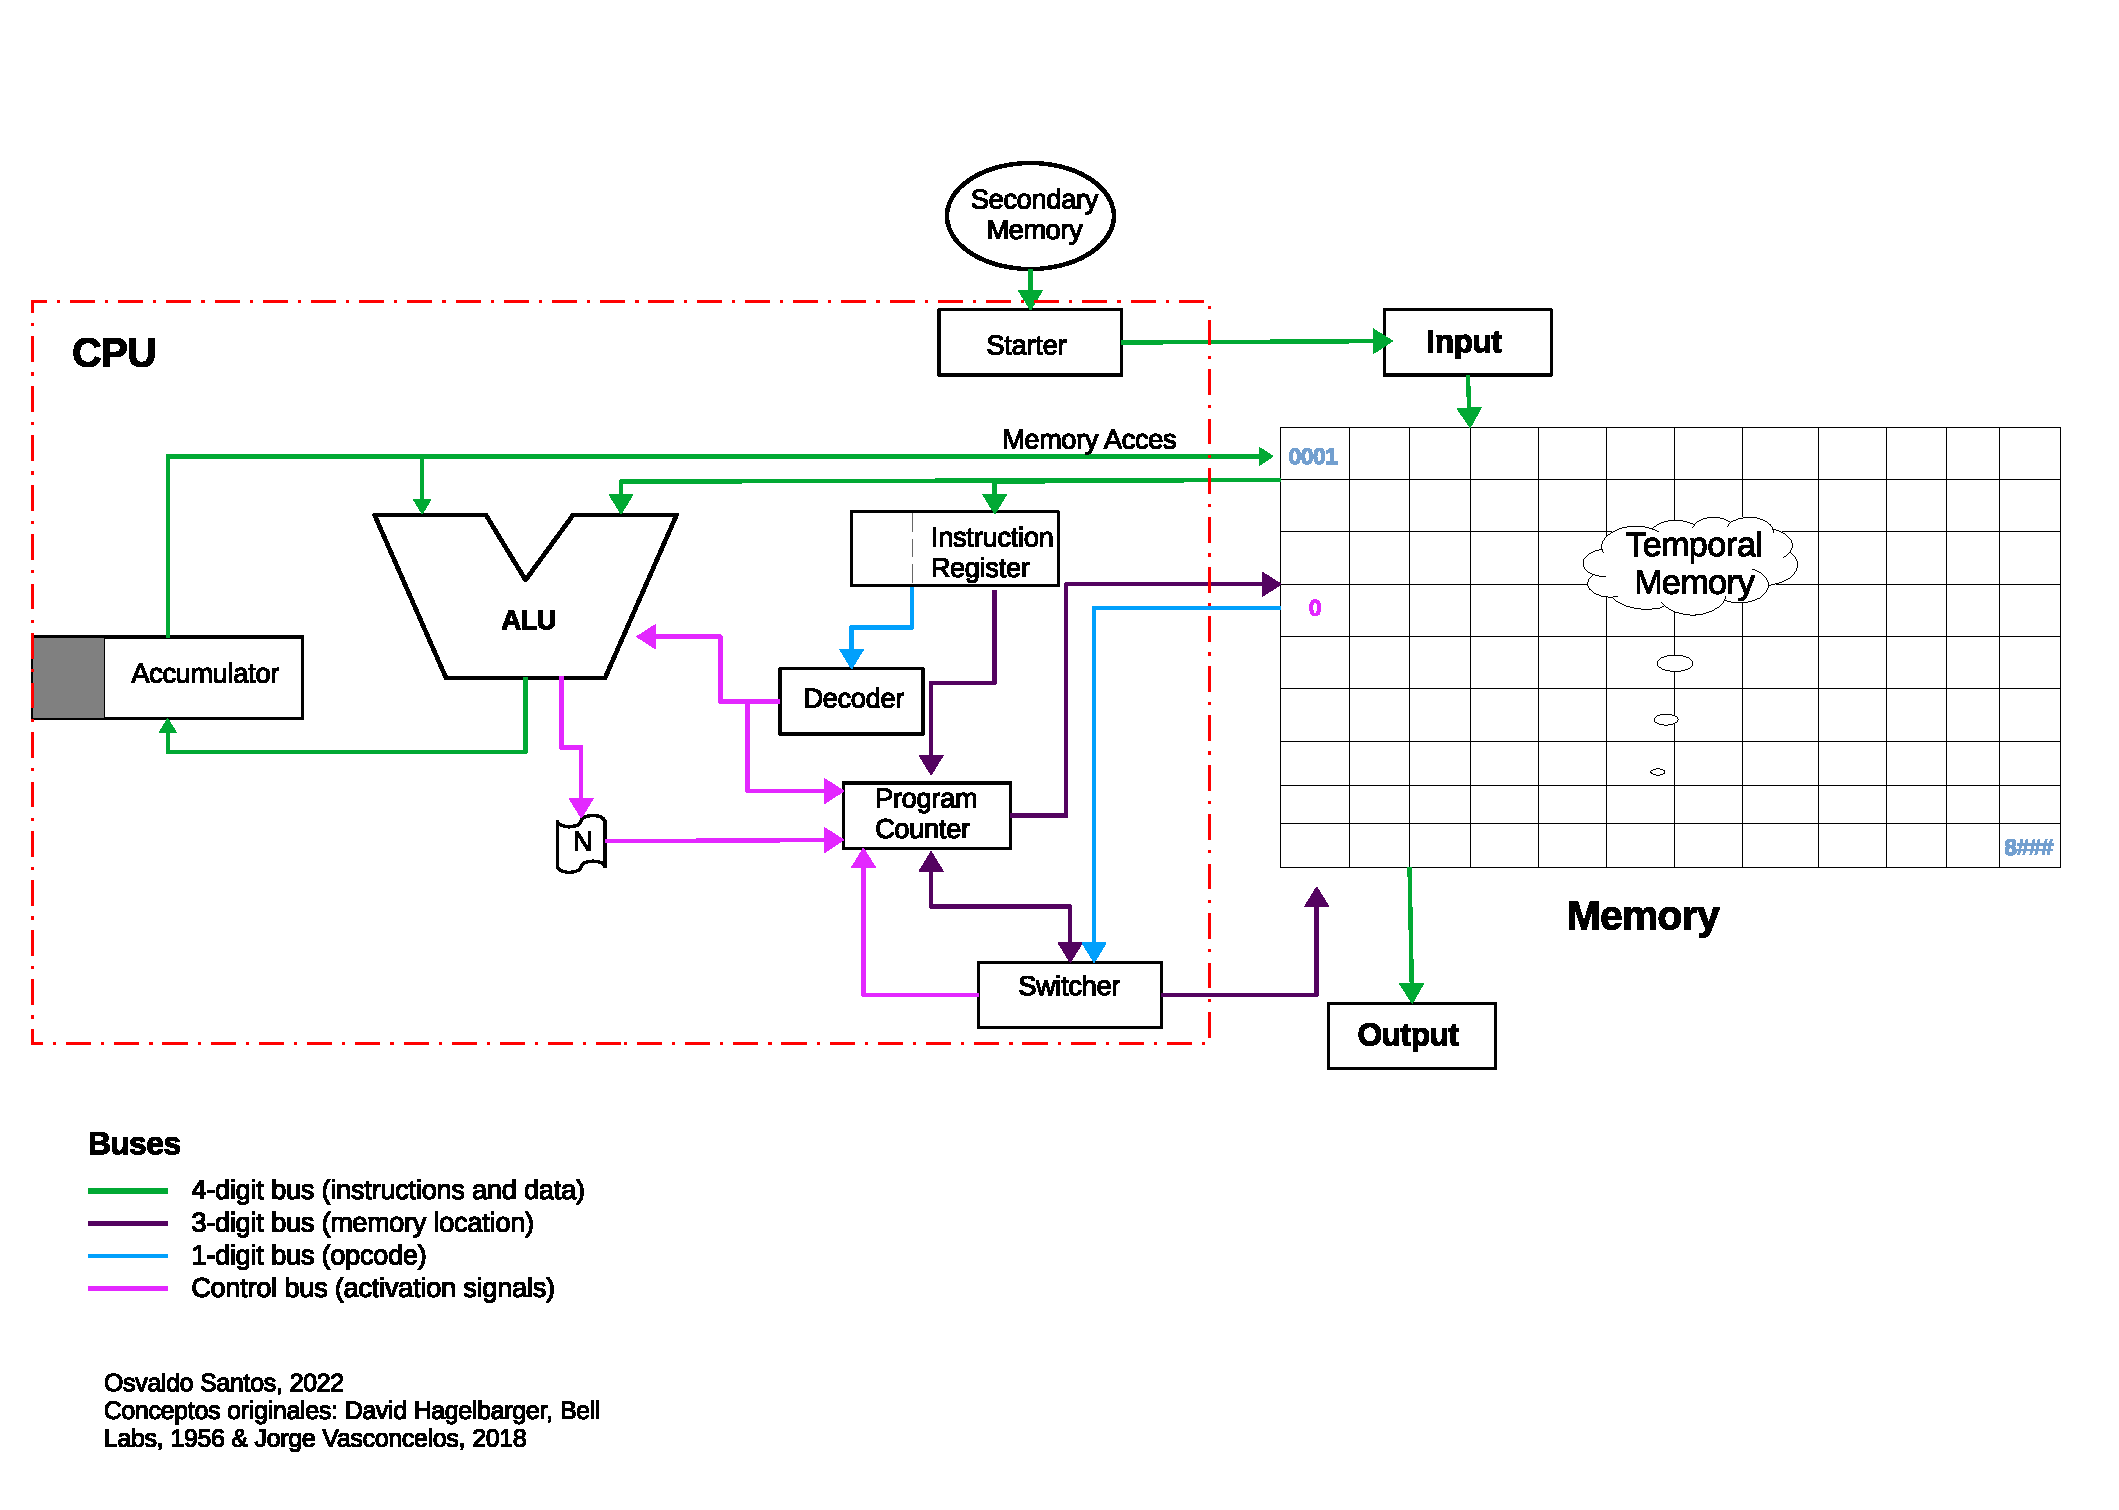
\includegraphics[scale=0.48]{media/CARDIACC/Arquitectura_diagrama_concurrente.eps}
			\caption{Diagrama de Arquitectura de E-CARDIAC C}
			\label{fig:diagarquiConc}
		\end{figure}
		
		
		Esto permite mantener varios elementos del modelo original sin cambios. Pero, podemos notar tres elementos nuevos, que a su vez
		incrementan el número de buses presentes en el modelo. Analicemos primero al que está conectado con el dispositivo de entrada (\textit{input}) 
		en la parte superior del centro. Este
		tiene por nombre \textbf{starter} (iniciador), y de igual manera, está conectado con otro elemento nuevo: la \textbf{secondary memory}, o 
		memoria secundaria.

  
		La memoria secundaria es la representación de lo que sería el disco duro en las computadoras actuales, pero más limitada, porque sirve 
		como un almacenamiento
		puntual para el sistema operativo, como si de una tarjeta de programas se tratase. Esta
		tiene conexión con el iniciador, mismo que se conecta al dispositivo de entrada, para que al iniciar la máquina lo primero que haga sea agregar 
		las instrucciones guardadas
		en la memoria secundaria a la cola de ejecución.
  
        De esta manera, podemos mantener simple el modelo, pero, a su vez, establecer una conexión
		con otra fuente de información diferente a la memoria principal. De esta forma logramos cargar el sistema operativo mínimo sin que ocupe espacio desde 
		el principio en la memoria RAM, tal cual sucede en las computadoras actuales. Con lo que conseguimos una mayor similitud entre el modelo
		y las computadoras del momento.
		
		
		El otro integrante de este nuevo modelo es el que tiene por nombre \textbf{switcher} (conmutador), que está en la parte inferior derecha del 
		área de la \textit{CPU}.
		Este elemento es la solución al problema de incluir un programa que requiere los privilegios para controlar las ejecuciones,
		ceder el control a otros programas y poder recuperarlo en un momento particular.
  
        Como se puede observar en la figura \ref{fig:diagarquiConc}, el conmutador tiene cuatro diferentes conexiones, siendo uno
		de los que más posee. Es necesario ya que la configuración de la máquina, para funcionar con un sistema operativo mínimo, establece
		que el SOM tendrá el control de los recursos, pero puede cederlos a otros procesos para que sean
		ejecutados. Sin embargo, los procesos de los usuarios pueden, a lo más, disponer de \textbf{N} ciclos para ejecutar sus
		operaciones, una vez terminados esos N ciclos el control de los recursos vuelve al SOM; el encargado de controlar estos saltos cada
		N ciclos es el conmutador. Esto con el fin de ir alternando las ejecuciones de los procesos del usuario: al principio se ejecutan las
		primeras N instrucciones del programa 1, luego las primeras N del programa 2, luego volvemos con las siguientes N del programa
		1 y así sucesivamente hasta terminar; ejecutando los procesos concurrentemente.
		
		Ya que el SOM no tiene límite en cuanto a los
		ciclos que puede requerir para ejecutar sus instrucciones, el conmutador necesita una bandera que indique si se están
		ejecutando instrucciones del SOM o del usuario. La bandera se encuentra en la dirección \#003, si el contenido es 1 significa que es instrucción
		del usuario, si el contenido es 0 significa que es del SOM. Así el conmutador necesita una conexión con la memoria para la bandera;
		otra con la misma memoria, pero para las direcciones; una para conectarse al contador de programa e indicarle cuando saltar y otra
		que le transmita la dirección a donde saltar al mismo contador de programa.
		
		
		Vamos a analizar estas conexiones del conmutador con más detalle. Para empezar 
		el conmutador cada \textbf{N} ciclos manda una señal (con el bus rosa) al contador de programa para que salte a la \textbf{dirección 
		de inicio del sistema operativo}. Esta dirección tiene que ser establecida en la configuración inicial de la misma arquitectura. Este salto lo hace siempre y cuando en la dirección
		\#003 el contenido sea $1$, pues es la bandera que indica que es tiempo de ejecución del usuario y por ende cada N ciclos los recursos 
		deben regresar al SOM. Si
		el valor fuese un $0$, como es por defecto, no haría esos saltos, puesto que significa que los recursos los tiene el SOM; el cual puede disponer
		de ellos sin límite al tener todos los privilegios posibles. Esta conexión entre el conmutador y la memoria principal para
		obtener la bandera se realiza a través de un 
		bus azul, pues solo requiere de un dígito.
  
        Otra conexión es una bidireccional al contador de programa, que le permite contar los ciclos que han sucedido desde que el SOM cedió el control, indicarle al contador de programa cuándo debe regresar los recursos al SOM, y a qué dirección
		debe saltar para devolver el control de los recursos. El \textit{conmutador} tiene un contador propio, el cual sigue al contador de programa, pero que se reinicia cada que la bandera de saltos, que se encuentra en \#003, cambia de valor.
        Para todo esto, se requiere un bus de color morado para transmitir las direcciones y datos, y uno de color rosa para mandar la señal
        de interrupción al contador de programa para que detenga su proceso natural.
  
        Una razón adicional para esta conexión bidireccional es que el \textit{conmutador} recibe del contador de programa la última dirección
		apuntada por el proceso del usuario, antes de que fuera ejecutada. Esto sucede debido a que, en ese momento, al cumplirse los N ciclos, se da la instrucción de regresar los recursos al SOM, y entonces esa última dirección es transmitida al \textit{conmutador}. La intención de esto es que, por medio de su conexión a la memoria principal (por el bus morado),
		la coloque en una dirección especial para que el SOM pueda recuperarla, y cuando regrese los recursos a ese proceso, pueda continuar
		justo en la instrucción que no pudo ejecutar.
		
		El sistema operativo mínimo, en su misma ejecución, lanza los procesos del usuario, y por ende, realiza los saltos necesarios para ceder los recursos. Pero antes de lanzarlos,		
		modifica el valor de la dirección $\#003$ a $1$, para que el \textit{conmutador} pueda regresar el control al SOM después de N ciclos aproximadamente. La aclaración de ``aproximadamente'' es porque
		una vez que se cambia el valor a $1$ por el SOM en la dirección que funge como \textbf{bandera de saltos}, aún ejecutará un par de instrucciones propias
		del SOM para lanzar el proceso. Por lo que en realidad el proceso del usuario tendrá $N-2$ ciclos disponibles antes de regresar los recursos.
		
		Por supuesto, con todos estos cambios hechos para poder instalar un sistema que administre la ejecución de procesos de forma concurrente, el lenguaje también
		requiere modificaciones, en su mayoría mínimas, pero que van orientadas a funcionar en conjunto con un sistema operativo.
		
		\subsection{Cambios en el lenguaje}
		
		Como ya leímos en secciones pasadas, el lenguaje de una máquina muchas veces es consecuencia de las posibilidades que el hardware le ofrece. 
		Pero
		también el lenguaje define ciertas necesidades del hardware, por lo que en la construcción de una computadora se necesita pensar en todos
		los elementos que interactuarán entre sí. 
  
        Para E-CARDIAC C agregamos un nivel adicional, la consideración del sistema operativo mínimo. Como
		podemos notar en la tabla \ref{tab:programing_language_ecc}, uno de los únicos dos cambios que se realizó es en la instrucción \textit{halt}. Esta está diseñada ahora para funcionar con un sistema operativo, ya que, por sí misma, no tendrá las capacidades completas que sí tendrá con un SOM.
        
        En la configuración inicial de la computadora se definirá la dirección  establecida como \textit{área de borrado} para el SOM, área que ocupa la instrucción \textit{halt} para finalizar procesos. Esto se debe a que ya no finalizará programas la instrucción, sino procesos, y es la razón por la cual
        esta instrucción no se entiende sin un sistema operativo. Con esto,
		podemos considerar que nuestro SOM es, en cierta medida, una capa de abstracción entre el código máquina puro y las instrucciones que usa el usuario en sus procesos.

		
		
			\begin{table}[h]
			  \centering
			  \begin{tabular}{|c|c|p{8cm}|}
			    \hline
		    	\textbf{Código de operación} & \textbf{Mnemotecnia} & \textbf{Definición} \\
			    \hline
			    0 & INP & Guardar datos en memoria.\\
			    \hline
				1 & LDA & Cargar en el acumulador información de la memoria.\\
				\hline
			    2 & ADD & Sumar al contenido del acumulador contenido de la memoria.\\
			    \hline
			    3 & BLZ & Saltar si la información en el acumulador es menor que cero.\\
			    \hline
			    4 & SHF & Mover d1 veces a la izquierda el contenido del acumulador y d0 veces a la derecha.\\
			    \hline
			    5 & OUT & Escribir en la salida el contenido de la memoria.\\
			    \hline
			    6 & STO & Guardar información del acumulador en la memoria.\\
			    \hline
			    7 & SUB & Restar información de la memoria al acumulador.\\
			    \hline
			    8 & JMP & Saltar y guardar el valor del contador de programa en la dirección \#999. \\
			    \hline
			    9 & HLT & Detener la ejecución del programa y saltar al área de borrado de procesos del SO, no importa el valor que los dígitos d0,d1 y d2 tengan.\\
			    \hline
			  \end{tabular}
			  \caption{Lenguaje de programación de \textit{E-CARDIAC C}.}
			  \label{tab:programing_language_ecc}
			\end{table}
 
		
		Si consideramos el dígito a extrema izquierda como \textit{d3}, y el resto de manera descendente
		hasta llegar a \textit{d0} en la derecha, tenemos que el dígito \textit{d3} tendrá el código de operación cuando se trate de una instrucción. 
		Para \textit{shift} esto será importante, puesto que, en esta instrucción solo importarán los dígitos \textit{d1} y \textit{d0}, ya que el 	
		\textit{d2} no representará nada. Se tendrá en \textit{d1} la cantidad de lugares que se desplazará el número a la izquierda, y 
		en \textit{d0} la cantidad de lugares que se desplazará a la derecha.
		
		El último cambio a destacar es que el valor del contador de programa, que se guardaba en la \#99 cuando se hacía un salto con la instrucción 
		\textit{jump}, ahora
		será guardado en la dirección \#999 para adaptarse a esta arquitectura. Aun con esto, para el resto de instrucciones
		el comportamiento no cambiará, solo que ahora tienen tres dígitos a la derecha que representan la dirección, ya que las
		direcciones
		ya no ocupan dos dígitos, sino tres.
		
		Con esto tenemos el diseño completo de la máquina, su arquitectura y su lenguaje. Ahora podemos dar el paso a escribir el sistema operativo 
		mínimo que
		pueda realizar las tareas que esperamos en este modelo. Sin embargo, como se mencionó, ya se había pensado en qué características necesitaba la 
		computadora
		para poder implementar un SOM.

		
		\subsection{Sistema operativo mínimo C: Aspectos generales}
		
		Ahora conocemos las necesidades particulares que se requieren para
		implementar un sistema operativo en nuestro modelo. El siguiente paso es construir ese sistema.
		 Por lo tanto, en el desarrollo de este sistema operativo
		mínimo, al que llamaremos \textit{SOMC}, está una lista de tareas que debe ser capaz de realizar para poder ejecutar de manera
		concurrente diferentes procesos; lo cual es la finalidad principal de su construcción.
		
		El diseño de este programa lo hice pensando en una arquitectura de mil celdas, pero que pudiese ser extensible a más. Para lograrlo, era 
		necesario
		que las direcciones no fuesen fijas en el diseño del programa. Por lo que usé variables para las direcciones, de forma que en
		el diseño puedo tener una dirección como \#s1, pero en la implementación esa dirección se transforma en \#801. Así, si tengo una
		instrucción de la forma \textit{1(s1)}, su mapeo será \textit{1801}.
  
        De esta manera, tenemos mucha flexibilidad al momento de escribir
		el código del programa. Cuando comencé, pensé que con menos de 100 celdas de memoria podría escribir todo el programa, por ende, que iniciara
		en la celda \#900 parecía razonable. Pero a medida que avancé,
		descubrí que no, y esta flexibilidad en cuanto a las direcciones me permitió seguir escribiendo para más de 100 direcciones sin tener que reescribir
		lo que ya tenía. Lo único que tenía que hacer es cambiar la dirección de inicio de mi programa, si antes \#s0, la dirección de inicio del SOM,
		era \#900, ahora sería \#800, y el resto aumentaría secuencialmente.
		
		Otra parte importante para mantener esta flexibilidad fue dividir el programa en diversos \textbf{segmentos}. El principal es el \textbf{núcleo} 
		del
		sistema operativo mínimo, y que lleva tal cual ese nombre. Otro es la \textbf{zona de procesos}, para almacenar el contexto de los
		procesos que se ejecutan en la máquina. También hay una \textbf{zona de variables}, que contendrá variables o constantes de uso 
		recurrente,
		para que el sistema operativo mínimo pueda guardar o consultar. Por último, un segmento llamado \textbf{preámbulo}, que contiene las primeras 
		instrucciones
		que se ejecutan cuando el SOM toma control de los recursos, y así prepara ciertas variables para que cuando el núcleo del SOM esté en ejecución,
		todas las variables estén en la posición correcta. Las ventajas de segmentar el programa son que se pueden cambiar las direcciones de inicio de 
		cada segmento sin afectar a los demás.

		
		Adicionalmente, el núcleo del SOM se fraccionó en etapas dependiendo de las tareas que realiza en cada parte, separándolas en:
		añadir proceso, actualizar proceso, borrar proceso, ejecutar proceso y gestión del arrancador (\textit{bootloader}). Para poder seguir todos 
		estos conceptos con más claridad
		  diseñé un diagrama de flujo, que se puede observar en la figura \ref{fig:diagramaSOMC},
		   en la cual cada etapa del núcleo está con un color diferente. Por el tamaño del diagrama es difícil apreciar lo que dicen las letras, por ende,
		en cada etapa que requiramos del diagrama se hará un acercamiento. Pero para entender
		las conexiones entre cada etapa esta figura es de mucha ayuda.
		

		\begin{figure}[p]		
			\centering
			
\includegraphics[width=\textwidth,height=\textheight,keepaspectratio]{media/CARDIACC/Diagrama_Flujo_SO.eps}
			\caption{Diagrama de flujo de SOMC}
			\label{fig:diagramaSOMC}
		\end{figure}		
		

		
		\subsubsection{Nomenclatura del diseño del código}
		
		Para explicar el código del sistema utilizaré, además del ya mencionado diagrama, imágenes como la de la figura \ref{fig:somcPreambulo}, donde
		se puede ver el código, así como una descripción de cada instrucción. A la izquierda está el ``nombre clave'' de cada dirección o grupo
		de direcciones, que es una descripción corta acerca de esas direcciones, y solo se coloca si es necesaria. Por ejemplo, en las instrucciones
		coloreadas de rosa hay un nombre clave que indica que es una bandera. En la siguiente columna tenemos la dirección de memoria, después
		la instrucción en lenguaje máquina y al lado la instrucción en lenguaje ensamblador. Para finalizar, en la parte derecha tenemos la descripción 
		completa de la instrucción, en caso de que esta sea necesaria.
  
        Cada segmento del SOM tendrá variables de dirección diferentes. Veamos el caso del
		preámbulo, donde las variables que indiquen las direcciones empezarán por una \textit{e} y continuarán de forma serial. En el recuadro
		de la figura \ref{fig:somcPreambulo} podemos ver cómo se usan. Si nos fijamos en la fila donde está la dirección \#e10, veremos la instrucción
		\textit{1(e)} que indica que se cargue el contenido de la dirección \#e0 en el acumulador. En la implementación, la variable
		de dirección será sustituida por una dirección real de la máquina y la instrucción \textit{1(e0)} pasaría a ser \textit{1890}.
		
		Así como para el preámbulo las variables de direcciones empiezan por \textit{e}, para la zona de procesos empezarán por \textit{p},
		en la zona de variables del sistema empezarán por \textit{c} y las del núcleo del sistema operativo empezarán por \textit{s}. De esta forma,
		también será rápido en el código identificar a qué zona está haciendo referencia la instrucción. 
  
        Por ejemplo, en la figura
		del preámbulo en la fila de la dirección \#e6, se encuentra una instrucción de la forma \textit{2(c13)}, lo que nos indica
		que trabajará con un valor de la zona de variables del sistema, debido a la letra \textit{c} que aparece en el interior
		de la instrucción. Examinándola, nos dice que se va a sumar al contenido del acumulador el contenido de la dirección \#c13, y tanto
		la descripción como el nombre clave brindan más información para entender mejor su funcionamiento.
		
		\begin{figure}[h]		
			\centering
			\includegraphics[scale=0.51]{media/CARDIACC/Preambulo.png}
			\caption{SOMC: Preámbulo}
			\label{fig:somcPreambulo}
		\end{figure}
		
		\subsubsection{Inicio de operaciones para el sistema operativo mínimo}
		%%Investigar lo que se dijo del bootloader antes
		
		El sistema operativo mínimo estará almacenado en la memoria secundaria, por lo que, para poder proceder con su carga 
		a la memoria principal de manera transparente al 
		usuario se
		requiere de un sistema de arranque (\textit{boot}). La forma de cargar datos de \textit{CARDIAC} está diseñada para 
		ser capaz de tener una
		especie de sistema de arranque si se siguen ciertas reglas al momento de cargar los datos, como
		comparten Fingerman y Hagelbarger en \cite{fingerman_instruction_1968}.
		En esta versión del modelo se han
		adaptado esas ideas para funcionar con una \textit{memoria secundaria} y un sistema operativo. 
		
		Para comenzar,
		las instrucciones que el \textit{iniciador} envíe desde la memoria secundaria a la cola de 
		ejecución deben estar en formato de tarjeta, es decir, en una lista de instrucciones o datos ordenados secuencialmente. Para los fines
		de este texto, una ``tarjeta'' será una lista de instrucciones que componen un programa. Así, un programa para sumar debe de
		tener una tarjeta con todas las instrucciones que requiera.
		
		Pero la tarjeta del sistema operativo mínimo, el primer programa en ser agregado, debe iniciar de la siguiente forma:

		\begin{center}
		\begin{minipage}{0\textwidth}
			\begin{verbatim}
				0002
				8000
			\end{verbatim}	
		\end{minipage}
		\end{center}
		
		Esto es 
		para formar un bucle al iniciar las operaciones de la máquina
		e iniciar así el sistema de arranque. Para lograrlo al principio siempre se 
		ejecuta la instrucción \textit{0001}, la cual se encuentra en la 
		dirección \#000, que es el comportamiento clásico del modelo.
		Si las dos primeras instrucciones en ser cargadas a la memoria son \textit{0002} y \textit{8000},
		lo que sucederá es que se
		cargará \textit{0002} en la dirección \#001 al terminar el primer ciclo (después de ejecutar la instrucción \textit{0001}). Por lo tanto,
		en el siguiente ciclo, donde la dirección apuntada será la \#001, se ejecutará la instrucción \textit{0002}, 
		que cargará en la dirección \#002 la instrucción \textit{8000}.
		Lo que generará un bucle para regresar siempre al inicio, puesto que cuando se llegue a la dirección \#002 se ejecutará la instrucción
		\textit{8000}, que indica el salto a la dirección \#000. Una vez formado este bucle el sistema de arranque se puede considerar
		iniciado, por lo que estas dos instrucciones solo son necesarias en el primer programa en ser cargado a la memoria.
		
		Con estas instrucciones de inicio conseguimos un sistema de arranque donde el resto de instrucciones de la tarjeta solo tengan que 
		seguir
		un formato de instrucciones pareadas para obtener una carga automática. Es decir, que se necesitan dos instrucciones para añadir un dato a la 
		memoria principal, la primera 
		instrucción define la dirección de destino
		de la segunda, y la segunda instrucción es la que será un dato o un elemento del programa a añadir a la memoria. 
		
		Abajo vemos cuáles serán 
		las siguientes instrucciones en la tarjeta del sistema operativo:
		
		\begin{center}
		\begin{minipage}{0\textwidth}
			\begin{verbatim}
			0003
			0000
			0004
			0000
			\end{verbatim}	
		\end{minipage}
		\end{center}
		
		El primer par de instrucciones que se ve es para cargar la bandera que indica si el proceso en ejecución es del usuario o del SOM.
		Como notamos, la primera instrucción del par establece que la segunda sea cargada en la dirección \#003 y que el valor cargado ahí sea un 0000. 
		Este valor se coloca por defecto para señalar que los recursos son del SOM. 
		
		Esto funciona así porque una vez iniciado el bucle
		la máquina estará apuntando a la dirección \#000 la cual, con la instrución \textit{0001}, estará esperando un dato para
		ser cargado en la dirección \#001; está vez ese dato será \textit{0003}. Lo que genera como consecuencia que en el siguiente
		ciclo, cuando el contador de programa apunte a la dirección \#001, se ejecute la instrucción \textit{0003}; lo que provoca que el siguiente
		dato ingresado por el usuario (o que esté en la cola), \textit{0000} en este caso, sea guardado en la dirección \#003. La siguiente dirección
		es la \#002, que contiene la instrucción \textit{8000}, por lo que saltara al inicio y podremos repetir este proceso una y otra vez.
		
		
		El siguiente par de instrucciones en ser leídas son el \textit{0004} y el \textit{0000}.
		El valor que será guardado en la dirección \#0004 
		 lo que nos indica es el identificador estático o, \textit{id 
		estático}, del proceso
		que se está ejecutando en ese mismo momento; más adelante se ahondará en este identificador.
		 El valor \textit{0} para este identificador no es solo un número por defecto, se coloca porque 
		justamente se está ejecutando el 
		\textbf{proceso 0}. 
  
		Se considera \textbf{proceso 0} a este sistema de arranque  porque para el SOM  será tratado como un proceso una vez que se haya completado la carga
		del sistema. De hecho, una vez terminada la carga del sistema
		la primera dirección en ser apuntada por el contador de programa será la \#000. Por lo tanto, el primer proceso en
		ejecutarse es el \textit{0}, y es reconocido por el identificador estático desde el inicio de la carga del sistema.
	    
	    Si bien es considerado un proceso más para el sistema, cuenta con algunas características especiales por su relevancia
	    para el SOM, como el hecho de que el proceso 0 es el único que no tiene límite de ciclos.
	     En el diagrama, los elementos relacionados con el proceso 0 se identifican con un color azul, son parte de la etapa  
	    \textit{ejecución del 
	    arrancador}.
		
		%% Apéndice 5
		El resto de los datos que tiene la tarjeta es todo el contenido  del sistema operativo mínimo. La tarjeta utilizada para cargar el sistema
		se encuentra completa en el apéndice E para su consulta, y básicamente consiste en pares de instrucciones para colocar cada segmento
		del sistema en su lugar.
		
		\subsubsection{Encendiendo la máquina}
		
		En la figura \ref{fig:eccApagada}, podemos observar  cómo será la máquina virtual para E-CARDIAC C, 
		la cual usaremos de guía para comprender 
		muchos de los aspectos del modelo y del sistema operativo mínimo. 
		Notamos que ahora, en la parte inferior derecha, ya no hay un espacio vacío como en la primera versión, sino que se muestra
		el contenido de la memoria secundaria, conformada por direcciones de esta memoria y su contenido.
  
        Si oprimimos \textit{Start},
		el contenido de la memoria secundaria se mueve a la cola de ejecución (\textit{Queue}), pero no desaparece de la memoria secundaria, como podemos
		ver en la figura \ref{fig:eccEncendida1}, ya que, al ser está una memoria no volátil, la información permanece estática. No cuenta como memoria 
		ROM porque es posible
		reescribirla, aunque de forma externa. La podemos pensar como una tarjeta que se puede cargar, similar
		a un disco de instalación.
  
        Como se notará en las imágenes, otra parte que cambió fue la del estatus de
		la máquina, que ahora tiene un campo llamado \textit{Starter}. En la máquina apagada tiene un valor de \textit{Waiting} (esperando), y 
		en la encendida, de \textit{Booted} (arrancada). Esto
		es porque al encender la computadora, el iniciador (\textit{starter}) coloca automáticamente la tarjeta de la memoria secundaria en la cola, 
		solo 
		es cuestión de dejar avanzar la ejecución para que la carga se complete. Por lo tanto, se considera que la máquina está ``arrancada''.

		\begin{figure}[h]		
			\centering
			\includegraphics[scale=0.32]{media/CARDIACC/ECARDIACC_apagada.png}
			\caption{E-CARDIAC C apagada}
			\label{fig:eccApagada}
		\end{figure}		
		
		\begin{figure}[h]		
			\centering
			\includegraphics[scale=0.32]{media/CARDIACC/ECARDIACC_encendida1.png}
			\caption{E-CARDIAC C durante el arranque}
			\label{fig:eccEncendida1}
		\end{figure}
	
		Además del \textit{Starter}, tenemos otros tres campos nuevos, los cuales nos ayudarán a ver quién tiene el control de los recursos y por 
		cuántos ciclos. El campo
		\textit{Limit of Cycles} (límite de ciclos) contiene el valor máximo de ciclos que tendrá un proceso del usuario antes que obligadamente tenga 
		que ceder
		los recursos de nuevo al SOM. En la implementación que se muestra tiene un máximo de 30 ciclos para cada proceso del usuario.
  
        El \textit{Counter SW} es el contador del conmutador y tiene
		un contador de ciclos, pero a diferencia de \textit{Cycle}, este se reinicia cada vez que el control de los recursos cambia de propietario. Si 
		está
		ejecutándose un proceso del usuario, cuando este contador alcance el límite de ciclos, el \textit{conmutador} saltará
		de inmediato al preámbulo del SOM para que este tome control de los recursos. Si es al revés, el contador solo nos servirá de indicador
		de cuántos ciclos lleva el SOM desde que controla los recursos, puesto que, como la bandera se encuentra en 0, si el control lo tiene el SOM, 
		el conmutador no podrá hacer ningún salto.
  
        Para saber quién tiene el control, también podemos ver el último campo: \textit{SW Status}, que es el estatus del conmutador y nos indicará 
        quién tiene
		el control de los recursos. En las imágenes lo tiene el SOM, por eso tiene un valor de \textit{SO}, si fuera un proceso del usuario, tendría \textit{User}. 

		Un aspecto a tener en cuenta es que si hay un proceso de usuario en ejecución, es decir el campo \textit{SW Status} tiene valor de \textit{User},
		cuando terminen sus ciclos y deba regresar el control al SOM, el salto que indica el conmutador es a una dirección del preámbulo 
		que cambiará el valor de la bandera de la dirección \#003.  Lo que ocurre como consecuencia es que
		las primeras instrucciones del preámbulo son consideradas aún como parte del proceso del usuario para el estatus, 
		porque
		en esas primeras instrucciones aún no se cambia el valor de la bandera, pero para el contador del conmutador esto ya se contempla como parte del
		proceso del SOM. Por ellos es importante destacar que el
		 valor del estatus va ligado completamente al valor de la bandera en la dirección \#003.
		
		Lo que sucede una vez que el sistema ha sido cargado en la memoria lo podemos ver en la figura \ref{fig:eccSOMcargado}, donde podemos notar que 
		el
		puntero está en la dirección \#000. Es decir, está esperando un dato para cargarlo en la dirección \#001, la cual ya tiene un dato que fue
		ingresado
		en algún momento durante la carga del SOM en memoria, pero que ahora es ``basura''.
  
        También podemos observar en la figura que las banderas están cargadas correctamente, y algo que puede llamarnos la atención
		es que el estatus del conmutador marca que el control de los recursos lo tiene el sistema operativo. Esto no es un error, porque parte de los 
		permisos especiales
		que tiene el proceso 0 es que no tiene un límite para ceder los recursos. Es una extensión del mismo sistema operativo. 
  
        Esto sucede porque es el proceso que permitirá
		al usuario cargar programas para que sean ejecutados, y no sería nada óptimo que cada \textit{N} ciclos tuviera que detener la carga del 
		programa para que otro se ejecute.
		La carga de programas por el usuario tiene el privilegio más alto entre los proceso y, solo el usuario tras haber cargado los procesos 
		deseados, cederá el control al SOM para que administre los recursos y empiece la ejecución de los procesos previamente cargados.
		
		\begin{figure}[h]		
			\centering
			\includegraphics[scale=0.32]{media/CARDIACC/ECARDIACC_socargado.png}
			\caption{E-CARDIAC C: Sistema operativo mínimo cargado}
			\label{fig:eccSOMcargado}
		\end{figure}
		
		
		\subsubsection{¿Cómo toma control el sistema operativo mínimo?}
		
		Como pudimos ver en las imágenes anteriores, a pesar de que para el \textit{conmutador} el control de los recursos actualmente está del lado
		del SOM, en realidad es el usuario quien los está detentando, aunque de manera limitada, hasta que decida cederlos al SOM. 
  
        En la figura \ref{fig:diagramaSOMC}, se nos presenta un diagrama de flujo (muy general) en el que podemos alcanzar a ver tres recuadros
		rosas, con una forma más inclinada que la de un rectángulo normal. Esto es porque son entradas de datos por parte del usuario, utilizadas en el 
		diagrama para ejemplificar que son las tres formas en que el usuario cede el control de los recursos al SOM. La primera es cuando
		se va a añadir un nuevo proceso y el usuario ordena el salto; la segunda, cuando el contador de programa salta automáticamente por medio del 
		conmutador; y la tercera,
		si se da la indicación de borrado de un proceso con la operación \textit{Halt}, es decir, si se lee la instrucción \#9000.
		
		
		En la figura \ref{fig:eccSOMCdiagent} apreciamos estas tres formas en que el sistema toma control de los recursos, y podemos observar que todas 
		van a instrucciones
		de color café. Esto sucede siempre, ya que antes de acceder al núcleo del SOM, es necesario pasar por el preámbulo, que se encarga de 
		las actividades 
		previas	para que el sistema operativo mínimo pueda funcionar con normalidad y seguridad.
		
		
		\begin{figure}[h]		
			\centering
			\includegraphics[scale=0.25]{media/CARDIACC/ecardiaccDiagrama_entradas.png}
			\caption{Formas de entrar al sistema operativo mínimo C}
			\label{fig:eccSOMCdiagent}
		\end{figure}
		

        \subsection{Sistema operativo mínimo C: Un nuevo proceso en la cola}
        
        Veremos en orden cómo el sistema operativo mínimo interactuará con los programas que queramos ejecutar en E-CARDIAC C. Para ello, 
        partiremos
		de un ejemplo práctico. Lo primero que haremos es añadir un par de procesos e iniciar su ejecución. Estos tendrán que actualizar
		su contexto en la zona de procesos, así como ser eliminados de ahí cuando hayan finalizado. Así, podremos observar todo
		el ciclo de vida de un proceso en la computadora.
  
		\subsubsection{Añadir un proceso nuevo: tareas del usuario }
		
			
        % El usuario añade el programa
		El programa que añadiremos es para imprimir números del 1 al 10, un programa con el 
		único fin de explicar el funcionamiento de la máquina, el cual se llamará \textit{pintador}. Tendremos tres versiones: 
		una que 
		iniciará después de la 		
		dirección \#100, otra que iniciará
		después de la dirección \#300 y otra después de la \#500. 
		
		Observemos la tarjeta de la versión 1 en la tabla \ref{tab:fragmentoContador1a10}, que utiliza direcciones 
		posteriores a la \#100. En ella observamos 
		un fragmento de la tarjeta que el usuario colocará en la máquina virtual para añadir este programa a la zona de procesos. La primera 
		instrucción de la tarjeta  es para indicar que se cargue 
		en la dirección \#110 la primera instrucción de \textit{pintador v1}. El resto de la tarjeta sigue el mismo concepto de instrucciones pareadas 
		visto antes.
		
		\begin{table}[h]
			  \centering
			  \begin{tabular}{|c|c|p{8cm}|}
			    \hline
		    	\textbf{Código máquina} & \textbf{Ensamblador} & \textbf{Comentarios} \\
			    \hline
				0110  & LDA 110 & Cargará la primer instrucción en 110 \\
				\hline
				1000 & LDA 000 & Primera instrucción del programa \\
				\hline
				0111 & LDA 111 & \\
				\hline
				6105 & STO 105 & Segunda instrucción del programa \\
				\hline
				...&...&... \\
 				\hline
				0122 & LDA 122 & Última dirección del programa \\
				\hline
				9000 & HLT 000 & Dato \\
				\hline
				0104 & LDA 104 & Asignar constante n \\
				\hline
				0009 & LDA 009 & Dato \\
				\hline
				0800 & LDA 800 & Cargar en 800 la dirección de inicio del nuevo proceso \\
				\hline
				8110 &  JMP 110 & Dato \\
				\hline
				8985 & JMP 985 & Saltar al segmento de añadir proceso del SO \\
				\hline
			  \end{tabular}
			  \caption{Fragmento de código  para imprimir números del 1 al 10}
			  \label{tab:fragmentoContador1a10}
			\end{table}
  
        %% Pendinte el añadido a la sección de S, que se comenta hasta más adelante
        Sin embargo, al final hay una sola instrucción que se sale de esta regla:
        la instrucción \textit{JMP 985}, que sirve para saltar directamente a la dirección
		donde el sistema operativo comenzará a añadir el programa a la zona de procesos. En ese momento, el usuario cede por completo el control
		al SOM para que la información del programa, que ya cargó en memoria, sea añadida a la zona de procesos y este se convierta en un 
		\textbf{proceso}. 
		Esta dirección, la \#985, es la única del sistema operativo mínimo a la que el usuario tiene permiso para saltar, puesto
		que el usuario tiene permisos restringidos en todas las direcciones propias del sistema operativo y sus segmentos.
		
		Para ver la tarjeta completa, podemos consultar la tabla \ref{tab:tarjetaContador1a10}, la cual se lee de arriba hacia abajo y de
		izquierda a derecha. En esta, se puede observar que todas las 
		instrucciones
		que se encuentran en la mitad, aquellas omitidas en la tabla \ref{tab:fragmentoContador1a10}, son efectivamente pares de instrucciones para ir 
		cargando el 
		programa en la memoria principal.
				
		
		
		
			\begin{table}[h]
			  \centering
			  \begin{tabular}{|c|c|c|}
			  \hline
				Pintador (p1) &Pintador (p2)&Pintador (p3)\\
			  \hline
			    0110	&	0116	&	0122	\\
				1000	&	2000	&	9000	\\
				0111	&	0117	&	0104	\\
				6105	&	6105	&	0009	\\
				0112	&	0118	&	0800	\\
				1104	&	1104	&	8110	\\
				0113	&	0119	&	8985	\\
				3122	&	7000	&		\\
				0114	&	0120	&		\\
				5105	&	6104	&		\\
				0115	&	0121	&		\\
				1105	&	8112	&		\\
				\hline
			  \end{tabular}
			  \caption{Tarjeta para cargar proceso para imprimir números del 1 al 10}
			  \label{tab:tarjetaContador1a10}
			\end{table}

   %% Actuar del sistema operativo(preámbulo)
            \subsubsection{Añadir un proceso nuevo: tareas del Preámbulo}
			
			El siguiente paso está del lado del sistema operativo, y lo primero que se necesita saber es a qué parte del sistema se salta con
			la última instrucción de la tarjeta del usuario. El
			salto es al preámbulo del sistema, como ya podíamos suponer por lo revisado, y más precisamente a la dirección que corresponde a la variable
			\textit{e14}. Así, podemos decir que, en nuestra implementación, el valor de \textit{e14} equivale a la dirección \#985. Si observamos la 
			figura
			\ref{fig:somcPreambulo}, donde empieza \textit{e14}, el nombre clave asocia a esta y las siguientes direcciones a la
			etapa \textbf{añadir un proceso}, lo que lo hace más claro. 
			
			Es en este punto donde también observamos la aparición de las \textit{variables del 
			sistema}. Podemos ver en la figura \ref{fig:somcVariablesSis} que hay 19 variables o constantes que el sistema usará a lo largo
			de su ejecución. En este momento nos interesan particularmente las que se usan en está parte del preámbulo,
			la variable \textit{c4} y la variable \textit{c16}; la primera es un \textbf{contador de los 
			procesos del usuario}, que por defecto tiene 0, pues se empieza con 0 procesos y el \textit{proceso 0} no se considera
			del usuario, por lo que no suma en el contador; la segunda contiene el \textbf{número máximo
			de procesos} que se pueden cargar en el sistema operativo. El número máximo para la implementación es 5; para establecerlo, en
            \textit{c16} se coloca el número máximo que queremos menos uno.
   
            Volviendo al preámbulo podemos ver por qué se hace ese ajuste para el máximo número de procesos. La primera acción del preámbulo
			es tomar el número máximo de procesos permitidos menos uno, restarle la cantidad
			de procesos que el usuario ha agregado y toma una decisión: si el resultado es menor que cero no se permite agregar más procesos
			y saltará
			al sistema de arranque, pues se ha alcanzado el número máximo de procesos; en caso
			contrario, saltará directamente a la etapa  \textit{añadir proceso}. 
			
			En el caso de que el usuario tenga 4 procesos agregados y se vaya a 
			añadir 
			otro (el quinto),
			\textit{c4} tendrá un valor de 4 y \textit{c16} de 4 también, por lo que el resultado de la resta entre ambos será 0, lo que permitirá 
			añadir el quinto proceso. En
			cambio, si el usuario ya tuviera 5 procesos, el resultado sería negativo y el condicional indicaría reiniciar en el proceso 0. Por lo tanto,
			si queremos como máximo 10 procesos ejecutándose de manera concurrente, hay que considerar este funcionamiento y colocar en \textit{c16} un 
			9.
			
						
			
			\begin{figure}[h]		
			\centering
			\includegraphics[scale=0.56]{media/CARDIACC/VariablesDelSistema.png}
			\caption{SOMC : Variables del sistema}
			\label{fig:somcVariablesSis}
		\end{figure}

  %% Nucleo del Sistema
            \subsubsection{Etapa \textit{Añadir proceso}: Validaciones previas y posteriores}
			%% Validaciones previas
			Ahora sabemos que desde el preámbulo se saltará al segmento del núcleo del SOM para añadir un nuevo proceso, puesto
			que hay 0 procesos del usuario y se permite añadir otro. El salto se realiza a la dirección \textit{s66}, la cual funciona para recordar
			que la letra ``s'' en las variables representa
			direcciones del núcleo del sistema operativo.
   
            Pero observemos
			primero el diagrama, con un acercamiento en la etapa de añadir un nuevo proceso, de la figura \ref{fig:diagAddnewprocess}. Después
			de pasar por la parte café del preámbulo con un resultado de ``No'' (en la figura \ref{fig:eccSOMCdiagent} se ve completo
			el rombo café a la izquierda de la misma), es decir no se ha alcanzado el máximo número de procesos,
			llega a otro condicional que pregunta si en realidad existe un proceso nuevo a añadir, pues hay que validar que no se haya saltado por
			accidente.
			
			La forma  en que el usuario deja una marca para indicar que sí hay un proceso por añadir, es colocando un valor
			en la dirección \#s0. La tarjeta del programa \textit{pintor v1} realiza esto en las dos últimas instrucciones previas
			al salto hacia el preámbulo. Este par contiene la instrucción \textit{0800}, que significa cargar un dato en la primera posición del núcleo 
			del sistema,
			y la instrucción \textit{8110}, que es la primera dirección del programa \textit{pintor v1}. Por lo tanto, este par de instrucciones
			sirve para colocar en \#s0 la dirección de inicio del proceso a ser cargado. Cabe aclarar que \#s0
			es \textbf{la única
			dirección del SOM en la que el usuario puede directamente escribir} sin restricciones.
   
            En la figura \ref{fig:somcGeneralnucleo}
			podemos ver que \textit{s0}, que en nuestra implementación es \textit{800}, tiene un valor por defecto de \textit{-0001}. Esto se debe a que 
			dicho valor indica que no hay un proceso por cargar, y cada vez que se termina de cargar un nuevo proceso, el contenido de esta dirección 
			regresa a su valor por defecto para preservar la integridad del sistema.
			

		\begin{figure}[h]		
			\centering
			\includegraphics[scale=0.4]{media/CARDIACC/DiagAddNewProcces.png}
			\caption{Diagrama de segmento para añadir un proceso}
			\label{fig:diagAddnewprocess}
		\end{figure}


			En caso de que el valor de \textit{s0} fuese negativo, si no hubiese proceso que agregar, 
			el flujo posterior al salto desde el preámbulo sería más corto,
			como se muestra en la figura \ref{fig:diagAddnewprocess}. El flujo comenzaría verificando el 
			valor del \textbf{Id organizer}, u ``organizador de identificadores'', que contiene el identificador del proceso que se está ejecutando. Si 
			el 
			valor es 0, es porque 
            la orden de añadir un nuevo proceso fue lanzada desde el cargador\footnote{Se utilizarán de forma indistinta ``proceso 0'', ``cargador'', 
            ``arrancador'', o 
            ``sistema de arranque'', aunque estos dos últimos se utilizarán principalmente cuando se trate de iniciar operaciones.}, por lo que regresaría 
            al proceso 0 mediante el recorrido más corto.
  
       
            Sin embargo, la última operación de la etapa \textit{añadir un proceso} (morada), continúa su flujo también en la condicional
            del organizador de identificadores. Así, en ambos resultados posibles del condicional ``¿Hay un nuevo proceso para añadir?'' 
			se termina revisando si la orden fue 
			lanzada desde el proceso 0. Esta verificación es relevante, ya que, si la orden de añadir un nuevo proceso no fue lanzada desde el proceso 
			0, como es lo normal, la etapa de gestión del proceso 0, toma mayor relevancia. 
			
			En el caso de 
			que no se haya lanzado la 
			orden
			desde el proceso 0, significa que un proceso del usuario dio la orden
   			de agregar un nuevo proceso. Si fue un proceso el que cedió los recursos, el sistema operativo tiene que elegir al siguiente 
   			proceso a ejecutar y no solo saltar al proceso 0. Si este es el caso, el diagrama nos indica que posterior
   			a la condicional del organizador se pasa a la siguiente
   			condicional de la etapa azul claro, donde se verifica si hay más procesos por lanzar con el \textit{id counter}, o ``contador
   			de identificadores''. Si no hay procesos por lanzar su valor será cero, por lo que reiniciará algunas variables  y saltará al proceso 0.
   			Pero,
   			si el resultado es diferente de cero, el flujo se enlazará con otra etapa del núcleo del sistema, que es el lanzamiento de procesos. Esta 
   			etapa y todo el tema de los identificadores lo veremos
			más adelante, es la parte que controla a quien ceder los recursos de la máquina.

			 \begin{figure}[H]		
				\centering
				\includegraphics[scale=0.55]{media/CARDIACC/SOMCGeneralNucleo.png}
				\caption{SOMC: Contenidos generales del núcleo}
				\label{fig:somcGeneralnucleo}
			\end{figure}
  

   %% Añadir procesos después de la validación
            \subsubsection{Etapa \textit{Añadir proceso}: Contexto del proceso}
			
			De regreso a la etapa morada del diagrama, después de verificar que hay un nuevo proceso por añadir, nos apoyaremos
			en las figuras \ref{fig:somcAddnewprocess} y \ref{fig:somcAddnewprocess2} para analizar los siguientes pasos de esta etapa. 

			Para añadir un nuevo proceso, y que el sistema operativo lo contemple, se deben actualizar valores tanto en la \textbf{zona 
			de 
			variables}
			como en la \textbf{zona de procesos}. En cuanto a las variables del sistema, vemos en la figura \ref{fig:somcAddnewprocess}
			que se actualiza el valor de \textit{c4} (en la dirección \textit{s70}); el contador
			de procesos aumenta en uno. Por otra parte, tenemos a \textit{c5}, el ``contador de direcciones''; este contador
			contiene la dirección del identificador del último proceso añadido, por lo tanto, contiene direcciones de la zona de procesos.
			La variable \textit{c5} tiene como valor por defecto a \textit{p0}, dado que toda variable que inicia con \textit{p} hace referencia a la 
			zona de 
			procesos.
			Precisamente, \textit{p0} es la dirección de inicio de la zona de procesos y contiene el identificador del proceso 0. 


		\begin{figure}[h]		
			\centering
			\includegraphics[scale=0.53]{media/CARDIACC/SO_AddNewProcess.png}
			\caption{SOMC: Añadir un proceso, parte 1}
			\label{fig:somcAddnewprocess}
		\end{figure}
		
				\begin{figure}[h]		
			\centering
			\includegraphics[scale=0.55]{media/CARDIACC/SO_AddNewProcess2.png}
			\caption{SOMC: Añadir un proceso, parte 2}
			\label{fig:somcAddnewprocess2}
		\end{figure}
			
			En la figura \ref{fig:somcZonaDeProcesos} podemos ver cómo está compuesta la zona de procesos. Llamaremos ``contexto del proceso'' a todas
			las variables asociadas al proceso, las cuales se almacenarán en la zona de procesos bajo un mismo identificador. E-CARDIAC C requiere
			de cinco variables para el contexto de sus procesos, siempre asociadas a un identificador. En la zona de procesos podemos observar
			el valor por defecto para \textit{p5} y \textit{p10}, el cual es
			\textit{-0001} en ambos, ya que son los 
			inicios de cada contexto, y ese valor por defecto indica que no hay un proceso en ese lugar.
			
			Un contexto inicia cada 5 direcciones, y un contenido negativo en su primera dirección, que es el identificador, significa que no hay 
			proceso en ese
			contexto. Por esa razón, al contador de direcciones se le añade un 5 en la dirección \#s72 (figura \ref{fig:somcAddnewprocess}),
			puesto que si está en \textit{p0} sumando un 5 se cambia al contexto
			de \textit{p5} (el segundo proceso). En nuestro caso es justo lo que hace: cambia a \textit{p5} el valor del contador de direcciones, porque ahora
			el último proceso es el que se encontrará en el contexto de \textit{p5}.
   
            Revisemos el resto de variables que están en el contexto del proceso. Primero tenemos a las dos más evidentes:
            el contador de programa, guardado en \textit{gpc}, y el acumulador, guardado en  \textit{gacc}. Estas variables contienen el último valor
            del contador de programa y del acumulador, respectivamente, antes de que el proceso cediera los recursos. Al crear el proceso, a 
            \textit{gpc} se le asigna la dirección de inicio del proceso, y a \textit{gacc} un cero.
            
             Adicionalmente, tenemos otras variables que 
            son muy importantes para el contexto, pero que quizá no son tan evidentes, como el \textit{gjump}. Esta variable guarda el último valor que 
            tuvo la última dirección de
			la máquina, \#999 en la implementación actual, durante la ejecución del proceso al que hace referencia. En caso de que se esté creando
			el proceso se coloca el valor por defecto que tiene el modelo. 
			
			Esta variable es necesaria debido a que el valor
			de la última dirección de la computadora cambia de acuerdo a las instrucciones de cada proceso y es vital guardarlo en
			el contexto de cada proceso para evitar fallas lógicas. Una posible falla sería tener un proceso A que dejó un \textit{8819} en la 
			última dirección, luego el proceso B dejó un \textit{8514}, y
			cuando vuelva el control al proceso A e intente usar el valor que hay en \#999 para ir a 
            la dirección \#819, termine en la \#514.
   
            Por último, para identificar a los procesos tenemos su ID principal, con el que
			inicia el contexto, y que tiene
			por nombre completo  \textit{ID counter}, ``ID contador'', o simplemente ``ID principal'' (aquel valor que va en \textit{p0},\textit{p5},...).
			 Este va en orden ascendente y también sirve para 
			contar cuántos procesos existen. Pero además tenemos el identificador
			estático, guardado en \textit{Static ID}, que mantiene un identificador inamovible para cada proceso.
			Más adelante, en la sección de borrado, veremos la importancia de este identificador
			estático y como se distancia del primero.
			 Por lo pronto, y desde este punto, siempre haremos la distinción entre cada identificador, pues sus funciones son distintas.		
			

			
		\begin{figure}[h]		
			\centering
			\includegraphics[scale=0.55]{media/CARDIACC/Zona_De_Procesos.png}
			\caption{SOMC: Zona de procesos del sistema operativo}
			\label{fig:somcZonaDeProcesos}
		\end{figure}

            \subsubsection{Etapa \textit{Añadir proceso}: Actualizando de información del proceso}
            
			Las figuras  \ref{fig:diagAddnewprocess}, \ref{fig:somcAddnewprocess}, y \ref{fig:somcAddnewprocess2} seguirán siendo
			nuestra guía para comprender cómo se va agregando la información faltante en el proceso. Primero se actualizan las variables del sistema, para 
			que este conozca cuántos procesos hay, dónde 
			están y cuál es el último
			contexto de la zona de procesos activo, es decir, con un \textit{ID contador} no negativo. Lo que vimos desde la dirección \#s68 hasta
			la \#s73 de la figura \ref{fig:somcAddnewprocess} y los dos primeros rectángulos morados de la figura \ref{fig:diagAddnewprocess}.
			
			
			Después, desde la dirección \#s74 hasta
			la \#s92, lo que hace es llenar el contexto del proceso. Se definió a \#p5 como la última dirección de inicio de un 
			contexto de proceso activo, por lo que el primer paso es asignar el número 1 como contenido de \#p5, ya que el \textit{ID contador} 
			es un 
			contador 
			de identificadores
			con valores ascendentes. Si agrego otro proceso, el contenido de \#p10 será un 2, y cuando borre ese proceso
			su contenido regresará a ser negativo, hasta que agregue otro proceso y su valor vuelva a ser dos. Esta estabilidad en el identificador 
			principal
			nos permite, con solo ese valor, conocer la cantidad de procesos que hay  y saber el lugar que ocupa cada proceso en la lista
			de procesos de la ZP, o zona de procesos.
			
			Para hacer la carga de los valores del contexto del proceso en su correspondiente lugar, es el mismo sistema operativo
			quien coloca las instrucciones para hacer la carga. Las instrucciones resaltadas en rojo en las imágenes del código 
			están así porque fue el mismo sistema quien las colocará. Es decir, como programador, no puedo colocar de manera estática la dirección
			\#p0 o \#p10 para agregar un proceso; tienen que ser direcciones dinámicas que coloque el SOM.
   
            Analicemos el caso del contador de identificadores. En la dirección
			\#s73 el valor del acumulador es \textit{p5}, es decir, la dirección de inicio del contexto del nuevo proceso. Como es una dirección sin 
			más,
			tiene un código de operación de 0, por lo que si en \#s74 le sumamos el valor que contiene \textit{c9}, que es un \textit{6000}, lo que 
			haremos
			será cambiar el código de operación que acompaña a la dirección \#p5 de un 0 a un 6, dando por resultado un \textit{6(p5)} en el 
			acumulador.
			Ese resultado, con la instrucción de \#s75 lo guardamos en la dirección \#s87. En la figura \ref{fig:somcAddnewprocess2}, 
			la dirección \#s87 tiene 
			un contenido genérico en color rojo con el código de operación \textit{6}, acompañado de un \textit{px}, indicando
			que se trata de una dirección tipo \textit{p}, que en nuestro caso sería la \#p5, pues es una dirección dinámica. 

			Dejamos un poco esa parte de las instrucciones y nos movemos hasta la \#s86, donde se carga
			en el acumulador el valor de \textit{c4}, que contiene el número de procesos que se han agregado hasta el momento. Cuando se apunte a \#s87,
			que tiene como contenido \textit{6(p5)}, se guardará el número 1 en \#p5, pues es el número de procesos que se han agregado hasta ese 
			momento de acuerdo con la variable \textit{c4}; ya que como recordaremos, las variables del sistema se actualizaron primero.
			
			En las imágenes, para simplificar el código, un \textit{px} siempre representará la dirección de un \textit{ID contador} del proceso, un
			\textit{px+1} el del \textit{gpc} del proceso, y así sucesivamente. Debido a que, como se puede ver, en el código no se cargan estos valores 
			en orden,
			y eso puede llegar a ser confuso. Con esta regla, podemos notar más fácilmente que en \#s92 se está cargando el contenido que deberá tener
			el \textit{gacc} en el contexto del proceso.	
			
			Al terminar con el ID contador se requiere colocar en \textit{p6}, que representa a la variable \textit{gpc}, la dirección
			de inicio del proceso antecedida por un código de operación \textit{8}, lo que ayuda en la simplificación del lanzamiento del proceso.
			La dirección de inicio del proceso es obtenida de la dirección \#s0, que fue donde se guardo dicha dirección por parte del usuario.
			En cuanto a la variable \textit{gacc}, que se encuentra en \textit{p7}, utiliza el valor por defecto 0, que será
			con el que inicie el acumulador del proceso cuando sea lanzado. La variable que
			no se actualiza es \textit{gjump}, en \textit{p8}, porque al inicio del proceso es razonable suponer que la última dirección de la máquina
			podría tener cualquier valor posible.
            
            Lo que sigue en el flujo  es modificar el identificador estático, que se debe cambiar
			tanto en la zona de variables del sistema como en el contexto del proceso que estamos agregando. Ya que, mientras el \textit{ID contador} 
			no guarda 
			ninguna
			relación con el proceso una vez que este termina, debido a que se reutiliza para otros una y otra vez, el identificador estático depende de un 
			valor
			en la zona de variables del sistema que es un serial, es decir, empieza en 0 y solo va aumentando a medida que agregamos procesos; este
			valor se encuentra en \textit{c15}. Así, el 
			proceso que
			tenga asignado el número 1 será el único que tenga esa asignación mientras la máquina esté encendida. 
			
			Para actualizar este valor lo primero que se 
			hace es aumentar
			el valor del contenido de \textit{c15} en una unidad y luego guardar ese valor en \#p9, que es la dirección donde se guarda el 
			\textit{ID estático}
			del nuevo proceso que se está añadiendo.
			
			Para finalizar, se reinicia el valor de \#s0 a un negativo, indicando que ya no hay un nuevo proceso por añadir. El flujo continúa
			hacia la etapa azul claro para validar si el proceso fue lanzado desde el proceso 0 y, en su caso,
			regresar al proceso 0, o si es necesario tomar el flujo más largo.
	        
	        Como notarán, en ningún momento se realiza cambio de bandera, ya que desde que el usuario agrega el programa hasta que
			el SOM lo añade a la zona de procesos, para el \textit{conmutador} el dueño de los recursos sigue siendo el SOM.
			
			
		
		\subsubsection{Práctica: añadir un proceso nuevo }		
		
			Analicemos en la máquina virtual cómo se añade un nuevo proceso. Estamos en la situación
			de la máquina iniciada, con el sistema operativo cargado y el contador de programa apuntando a  la dirección \#000,
			esperando para cargar un nuevo proceso. Pero, si observamos los valores con los que ha sido iniciada la computadora,
			en la figura \ref{fig:eccSOMcargado}, veremos algo interesante. En las últimas dos casillas superiores, que
			son listas desplegables, tenemos un \textit{100}, que hace referencia al número de celdas, y \textit{Instant}, que hace 
			referencia a la velocidad a la que cada ciclo se completa.
			
			A diferencia del primer modelo, en este la computadora no puede tener 
			\textit{100} 
			celdas de memoria, ya que cuando se inicia la máquina virtual,
			esta realiza una validación sobre las celdas indicadas en la lista desplegable, y verifica si son suficientes para el tipo de procesos que 
			llevará 
			a cabo. 
			\textit{E-CARDIAC C}
			solo puede funcionar con mil celdas o más; por esa razón, si la lista desplegable tiene un valor menor, la
			máquina se iniciará con el mínimo permitido, dejando en la lista desplegable el valor que ignoró.

        \begin{figure}[h]		
			\centering
			\includegraphics[scale=0.54]{media/CARDIACC/cardiaccProgramaEnDeck.png}
			\caption{E-CARDIAC C: Programa en \textit{deck mode}}
			\label{fig:eccProgramaenDeck}
		\end{figure}		
   
            
   
            En
			la figura \ref{fig:eccProgramaenDeck} observamos la máquina cargada nuevamente, y ahora si tiene el valor de \textit{1000} celdas en la 
			lista 
			desplegable. Además,
			en la figura \ref{fig:eccProgramaEnCola} podemos ver una velocidad diferente
            en la parte superior derecha;
			tiene el valor de \textit{Normal}, una velocidad en la que podemos apreciar los cambios y cómo se va ejecutando cada instrucción. Los 
			cambios de velocidad se pueden aplicar en cualquier momento del proceso dependiendo de las necesidades del usuario. Sin embargo, el cambio 
			en la 
			cantidad 
			de celdas solo puede efectuarse al iniciar la máquina.
			
			En esa misma figura, la \ref{fig:eccProgramaenDeck}, podemos ver en el modo de tarjetas una lista de instrucciones en texto
			escrita por el usuario,
			previo a oprimir el botón \textit{Add Card}. Una vez que se oprime el botón, esa tarjeta es trasladada a la
			cola, y lo podemos ver en la figura \ref{fig:eccProgramaEnCola}, donde aparece una lista de instrucciones que están siendo transmitidas a la 
			memoria principal desde la cola.

		\begin{figure}[h]		
			\centering
			\includegraphics[scale=0.54]{media/CARDIACC/eccProgramaenCola.png}
			\caption{E-CARDIAC C: Programa en cola}
			\label{fig:eccProgramaEnCola}
		\end{figure}	
		
		Luego, en la figura \ref{fig:eccAddNewProcesInst}, observamos que se vació la cola y la instrucción que se va a ejecutar 
		es para saltar al preámbulo y añadir un nuevo proceso a la lista. En este punto, el proceso de la carga del programa se ha completado,
		y lo podemos ver en la figura \ref{fig:eccPrograma1Cargado}, donde se observa el programa cargado en
		memoria. Cuando el sistema termina de agregar los datos de este
		programa a la zona de procesos es cuando, en sí, se convierte en un proceso, ya no son solo instrucciones de código. El contexto del proceso 
		es cargado por el sistema operativo después de que la instrucción 8985 es ejecutada y salta la etapa de añadir proceso, una vez
		concluida esa etapa todas las variables que necesita gestionar el SOM para la ejecución segura del proceso están listas.
        \begin{figure}[h]		
			\centering
			\includegraphics[scale=0.54]{media/CARDIACC/eccInstAñadirProceso.png}
			\caption{E-CARDIAC C: Instrucción para añadir proceso}
			\label{fig:eccAddNewProcesInst}
		\end{figure}

        \begin{figure}[h]		
			\centering
			\includegraphics[scale=0.25]{media/CARDIACC/eccPrograma1Cargado.png}
			\caption{E-CARDIAC C: Programa 1 cargado en memoria}
			\label{fig:eccPrograma1Cargado}
		\end{figure}	
  
        En la figura \ref{fig:eccZPProceso1}
		observamos el contexto del \textit{proceso 0}, que inicia en la dirección \#769, y también el del \textit{proceso 1}, que inicia en la dirección 
		\#774.
		El contexto del \textit{proceso 1} cuenta con: un \textit{ID contador}
		con un valor de 1, un \textit{gpc} que indica la dirección de inicio del proceso, un \textit{gacc} con ceros en su valor inicial,
		el \textit{gjump} con el valor por defecto que se tiene para la dirección \#999, y  un 1 para el ID estático, puesto que es el primer 
		proceso que se está agregando. Notamos también que la dirección \#779, el siguiente inicio del contexto de un proceso, tiene un valor de -1, 
		ya que no hay otro proceso más hasta este 
		momento.
		
		\begin{figure}[h]		
			\centering
			\includegraphics[scale=0.45]{media/CARDIACC/eccZonaProcesosPrograma1.png}
			\caption{E-CARDIAC C: Proceso 1 cargado}
			\label{fig:eccZPProceso1}
		\end{figure}	
		

		Para finalizar, agregaremos los otros dos \textit{pintadores}, que iniciarán en 
		\#310 y \#510, 
		respectivamente. Como una vez que se termina de agregar un proceso se regresa al proceso 0, podemos repetir el procedimiento sin ningún problema
		hasta alcanzar el número máximo de procesos. En la figura \ref{fig:eccTresProcessoAgregados} vemos la zona
		de procesos después de agregar estos dos, donde ahora el identificador de \#799 es un 2, y el de \#784 es
		un 3. Los tres procesos que agregamos tienen casi los mismos valores de arranque en su contexto, salvo las direcciones de inicio
		y sus identificadores.
		
		
		\begin{figure}[h]		
			\centering
			\includegraphics[scale=0.45]{media/CARDIACC/eccZP3procesosadded.png}
			\caption{E-CARDIAC C: Tres procesos agregados }
			\label{fig:eccTresProcessoAgregados}
		\end{figure}					
		
		\clearpage
		
		\subsection{Sistema operativo mínimo C: Lanzamiento de procesos}
  
		
		
		Si nos fijamos atentamente en el diagrama de flujo principal, notaremos que no hay una entrada que diga algo como ``ejecutar proceso''. 
		Una
		de las entradas al SOM es para añadir un proceso, otra cuando el contador de programa salta en automático y la tercera cuando se borra
		un proceso. Entonces, ¿cómo empezamos la ejecución de los procesos que tenemos cargados? La respuesta está en la última entrada mencionada y
		en características especiales del proceso 0. 
		
		Lo que el usuario tiene que hacer para iniciar la ejecución de los procesos
		que ha cargado es colocar en \#001 el valor \textit{9000}, la instrucción para detener un proceso, en este caso, el proceso 0. Lo que hace 
		después
		es saltar al preámbulo, por lo que hay que revisar las figura \ref{fig:somcPreambulo}
		y \ref{fig:diagZoomPreambulo} para ver en más detalle las instrucciones que ejecuta para ``finalizar''
		el \textit{proceso 0} y saltar al núcleo del SOM. Una vez en los recursos los ha recuperado el SOM comienza su tarea de administrar
		los recursos para decidir que procesos del usuario ejecutar.
		
		\subsubsection{Acciones del usuario y del preámbulo para lanzar un proceso}
  
		Después de ejecutar una instrucción \textit{Halt}, el salto es directo a la
		dirección \#e1, que sigue exactamente el mismo flujo que se sigue cuando el contador de programa salta de forma automática.
		Podemos seguir el flujo en la figura \ref{fig:diagZoomPreambulo} y el código en la \ref{fig:somcPreambulo}. Lo primero
		que se realiza es guardar en una variable del sistema el último valor que el acumulador del proceso tuvo antes de ceder los recursos. Después, 
		cambia la bandera 
		para que 
		ya no permita 
		saltos, y a continuación, guarda en otra variable del sistema el último valor que tuvo el contador de programa cuando
		el proceso estaba en ejecución. 
		
		Este valor se
		puede guardar
		gracias a que el conmutador en automático, cuando da la indicación de saltar al preámbulo, coloca en \#e0 el último valor que el \textit{pc}
		tuvo 
		durante el proceso de usuario. Mientras que si fue la instrucción
		\textit{halt} la que indicó el salto, el conmutador coloca un valor negativo en \#e0.

		%% Agregar en que imagen se puede seguir esto			
			
        \begin{figure}[h]		
			\centering
			\includegraphics[scale=0.4]{media/CARDIACC/diagPreambulo.png}
			\caption{Acercamiento al preámbulo en el diagrama}
			\label{fig:diagZoomPreambulo}
		\end{figure}
  
        La siguiente acción es guardar el valor del \textit{gjump}. Para ello, se toma directamente el valor del
		contenido de \#999. Este valor no ha sido contaminado, ya que
		los saltos hacia \#e1 por parte del conmutador y de la instrucción \textit{halt} no dejan ninguna marca en \#999.
		Entonces, cuando el apuntador llega a \#e8, simplemente toma el
		valor de \#999 y lo guarda en la zona de variables del sistema, más precisamente en \#c14, para resguardarlo.
  
        Por último, lee el valor de \#e0 (marca de \textit{halt}), y si es negativo, salta a la etapa de borrado;
		en caso contrario, salta a la dirección de actualización (más adelante revisaremos esa etapa).
		 En este caso, \#e0 es negativo, por lo que saltará a la etapa de borrado.

		Si ahora nosotros colocáramos \textit{900} en la dirección \#001 de la máquina virtual estaríamos ordenando la ejecución de los procesos
		y el ``borrado'' del proceso 0.
		En la figura \ref{fig:eccPreamHaltP0} podemos ver los efectos de realizar está acción 
		en la dirección \#950, que es la dirección \#e0 en la implementación,
		y ahora tiene un valor negativo. Por lo tanto, cuando llega
		al condicional en \#961 (\#e11) salta la dirección \#963, la cual contiene la instrucción para saltar a la etapa de borrado. 
		
		Si observamos 
		el diagrama en las figuras \ref{fig:diagZoomPreambulo} y \ref{fig:diagramaSOMC}, notaremos que es en esta parte donde 
		la flecha (el sí del rombo café)  sale de la etapa del preámbulo hasta el extremo izquierdo, donde está la etapa de borrado.

		
		\begin{figure}[h]		
			\centering
			\includegraphics[scale=0.4]{media/CARDIACC/eccPreambuloHaltOpP0.png}
			\caption{ E-CARDIAC: Preámbulo después de una detención en P0}
			\label{fig:eccPreamHaltP0}
		\end{figure}
		
		\subsubsection{Etapa \textit{borrar proceso}: Características especiales para el proceso 0}
		
		En el diagrama de la figura \ref{fig:diagBloqP0} vemos como llega una flecha al rectángulo que dice ``Obtener s1''. Esta flecha
		es la que salió del rombo café, de la figura \ref{fig:diagZoomPreambulo}, que dice ``¿La marca indica que fue un fin de proceso?''.
		Una vez que se llega a la etapa de borrado, la primera acción
		es el respaldo de una variable del sistema, pero inmediatamente después está la condicional que pregunta si la instrucción
		de borrado fue ejecutada desde el \textit{proceso 0}. Si no lo fue, continúa con la ejecución normal para
		borrar el proceso. En caso contrario, salta a la etapa de \textit{gestión del proceso 0} (en color azul claro),
		donde el proceso es bloqueado para que se puedan ejecutar otros. Por lo tanto, \textbf{el proceso 0 no es borrado},
		sino que al ser bloqueado, permite la conexión con la etapa del lanzamiento de procesos. Es por eso que, para lanzar los procesos que se han 
		cargado, el usuario tiene que escribir la instrucción \textit{halt} en el \textit{proceso 0}.

        
        %% Segmento s1
        Como
		el bloqueo del proceso 0 pasa necesariamente por la parte que recupera el valor de \#s1 (\#801 en la implementación), es un buen momento para 
		entender bien el funcionamiento de esta variable que ya hemos visto con anterioridad. Si observamos la figura \ref{fig:somcGeneralnucleo}, podemos
		ver que en el comentario ya se nos da una pequeña explicación de lo que es: el valor que guarda esa dirección siempre será la dirección
		del \textit{ID contador} del último proceso de usuario que se ha ejecutado, con un código de operación \textit{6}. Para simplificar, 
		usaremos la nomenclatura
		\textit{6-dir} para referirnos a una dirección con código de operación 6;
		se utilizará como prefijo el código de operación que tiene la dirección a la que hacemos referencia, y como sufijo
		la palabra \textit{dir}, haciendo referencia a dirección.
  
        Observemos ahora la
		figura \ref{fig:somcBorrar1}, que muestra el inicio de la zona de borrado. Lo primero que se realiza es obtener el valor de \#s1, 
		para que sea convertido
		en una \textit{1-dir}, es decir, una dirección con un código de operación \textit{1}. Si no se trata del \textit{proceso 0}, este cambio
		será útil. El siguiente paso es  obtener el \textit{ID contador} del proceso que se estaba ejecutando y verificar si es el proceso
		0; en caso de que lo sea, salta a la etapa de gestión del \textit{proceso 0}. En caso de que no sea el proceso 0 se verá la utilidad
		de tener la dirección en 
		la forma \textit{1-dir}, ya que esta se guarda en 
		la dirección \#s29, para
        que, cuando se ejecute esa instrucción, se obtenga el contenido de la dirección de la zona de procesos
        a la que hace referencia, que será el \textit{ID contador} del proceso que se requiere borrar.
  
        En este caso, como sí es el proceso 0, salta a la etapa azul claro en la dirección \#s98 para bloquear el proceso, y no 
		para borrarlo. Al bloquearlo, se impide su ejecución infinita y se permite que otros procesos se ejecuten hasta que sea necesario que este 
		proceso vuelva a ejecutarse.

        \begin{figure}[h]		
			\centering
			\includegraphics[scale=0.42]{media/CARDIACC/diagBloquearProceso.png}
			\caption{ Acercamiento a la parte del bloqueo al proceso 0}
			\label{fig:diagBloqP0}
		\end{figure}
  
	   
		Si observamos  la figura \ref{fig:somcNuceloP0}, podremos notar que en \#s98, dirección a la que salta el proceso de borrado, primero 
		se verifica si hay 
		más procesos. Para verificar que no existen más procesos
		se consulta la variable del sistema \#c4, que contiene un \textbf{contador de identificadores general}, que guarda el valor del 
		\textit{ID contador} más alto de los que
		se encuentran en la zona de procesos. Si este tiene un valor de cero, quiere decir que no hay más procesos, y lo que haría es regresar al 
		proceso 0.  Para seguir estos puntos en el diagrama podemos ver las figuras \ref{fig:somcEtapaAzulClaro} y \ref{fig:somcEtapaAzulClaro},
		que presentan un acercamiento a la etapa de gestión del proceso 0.

        \begin{figure}[H]		
			\centering
			\includegraphics[scale=0.53]{media/CARDIACC/SO_Proceso0.png}
			\caption{ SOMC segmento del proceso 0}
			\label{fig:somcNuceloP0}
		\end{figure}
		
		\begin{figure}[h]		
			\centering
			\includegraphics[scale=0.33]{media/CARDIACC/diagEtapaAzulClaro.png}
			\caption{ E-CARDIAC C: Etapa gestión del proceso 0}
			\label{fig:somcEtapaAzulClaro}
		\end{figure}
		
		\begin{figure}[h]		
			\centering
			\includegraphics[scale=0.4]{media/CARDIACC/diagEtapaAzulClaro2.png}
			\caption{ E-CARDIAC C: Etapa gestión del proceso 0 final}
			\label{fig:somcEtapaAzulClaro2}
		\end{figure}

  
  
        En la misma figura (\ref{fig:somcNuceloP0}),
		está la condicional de salto a \#s141, el salto que se realiza cuando no hay más procesos. En esa tabla hay una continuación directa de la dirección 
		\#s100 a 
		la \#s141, puesto que entre esas dos direcciones está la zona
		de lanzamiento de procesos, a la que el flujo continuará si hay procesos para lanzar, pero es más útil ver toda la etapa de gestión del proceso
		0 junta. 
		
		Lo que hace el flujo cuando continúa en
		\#s141 es reiniciar los valores del \textit{organizador de ID} (\#c7) y del \textit{organizador de direcciones} (\#c6);
		 más adelante revisaremos que función tienen en el modelo. También coloca en la dirección 
		\textbf{\#004} el valor de 0, ya que ahí se encuentra el valor del \textbf{identificador 
		estático} del proceso que se está ejecutando, en este caso será 0; esta dirección, asimismo, está reservada para el SOM. 
		Posteriormente, salta de 
		regreso al proceso 0.
		
		
		
		
		En caso de que sí haya más procesos a ejecutar, es decir que 
		el \textit{ID contador general} de la zona de variables del sistema tiene un valor mayor a 0, continúa la
		ejecución en la etapa de lanzamiento de los procesos.

		
		\begin{figure}[h]		
			\centering
			\includegraphics[scale=0.53]{media/CARDIACC/SO_Borrar1.png}
			\caption{ E-CARDIAC C: Borrado de proceso parte 1}
			\label{fig:somcBorrar1}
		\end{figure}
		
		
		


		\subsubsection{Etapa \textit{lanzamiento de procesos}: administración de procesos a ejecutar }		
	%% Funcionamiento del lanzamiento de proceoss	
		En este caso, la ejecución continuará en la etapa naranja del diagrama, en las direcciones que están entre \#s100 y \#s141, debido a que sí 
		hay más procesos para ejecutar. Como vemos en
		la figura \ref{fig:diagLanzProce}, continuamos en la etapa naranja después de verificar que el \textit{ID contador} no es cero
		en la etapa azul claro. 
		
		Aquí,
		las variables del sistema que serán muy importantes son las que están entre \#c3 y \#c7, dado que con estas 
		\textbf{el sistema puede controlar el orden de la ejecución
		de los procesos}		
		 y conocer las direcciones necesarias para lanzar los procesos de forma correcta; es decir, son las direcciones para encontrar
		el contexto del proceso. 
  
        Si consultamos la figura \ref{fig:somcVariablesSis}, observamos que en \#c3 se guarda siempre la dirección de inicio de la
		zona de procesos propios del usuario. Por esa razón contiene un \#p5 y no un \#p0, porque el \textit{proceso 0} es un proceso del SOM. La 
		dirección de inicio de la zona de procesos se decide en la implementación del sistema operativo.
  
        Después, en \#c4, como ya habíamos visto, tenemos el \textit{ID contador general}, o \textit{id counter} en los diagramas, que
		contiene el valor máximo de los contadores que están en la zona de procesos; su valor por defecto es 0, porque ese es el máximo al inicio. 
		Después de agregar tres procesos 
		en nuestra implementación, tiene un valor de 3. La variable \#c5 es su símil, pero en lugar de tener el identificador mayor
		de la zona de procesos, tiene la dirección de ese \textit{ID contador}; 
		es decir, tiene la dirección del último \textit{ID contador} de la zona de procesos
		que no es negativo.
  
        De esta manera, podemos conocer el último proceso. Sin embargo, para conocer la información del proceso a ejecutar necesitamos de los 
        \textbf{organizadores}: \#c6 y \#c7. Estos, en lugar de ser ``contadores''
		de identificadores y direcciones, contienen la dirección del \textit{ID contador} del proceso que se va a ejecutar y el valor de ese 
		identificador, respectivamente.
		
		
		Con todo esto, podemos lograr una concurrencia de procesos. Primero, se colocan los valores 
		del proceso a ser ejecutado en los
		\textbf{organizadores} \#c6 y \#c7, con ello, se puede tener acceso al contexto completo del proceso y ejecutarlo. Cuando
		el proceso alcance el límite de ciclos permitidos, se regresa 
		a la zona de lanzamiento
		y se aumenta el valor de los ``organizadores'' para ejecutar el siguiente proceso en cola. 
		
		En
		este sistema, se sigue un paradigma \textit{FIFO: First Input First 
		Output}, 
		es decir, el primero que entra es el primero que se ejecuta, 
		y así sucesivamente hasta llegar al último y detectar que ya no hay otro después. En 
		ese punto, se reinicia el lanzamiento en el proceso 1 y se continua de la misma forma hasta que terminen su ejecución todos los procesos.
		En ese momento, se reinician los organizadores para ir al proceso 0, puesto que mientras se estén ejecutando procesos del usuario, los organizadores
		no regresaran a lanzar el proceso 0; solo irán de 1 a n, 1 a 3 en nuestro ejemplo. 
		
		Eso significa que una vez que agregues los procesos
		que necesites y des la orden de ejecutarlos no podrás agregar ninguno nuevo hasta que termine la ejecución los procesos
		agregados. Cuando la ejecución de estos procesos termine, el SOM regresará el control de los recursos al proceso 0 y podrás agregar un nuevo
		proceso.

  %% Código para lanzar procesos nuevos
  		\subsubsection{Etapa \textit{lanzamiento de procesos}: análisis del código }
		
		En la figura \ref{fig:somcLanzamientoP1}, podemos seguir  los pasos para el lanzamiento de procesos en código.
        Empieza con el aumento de los organizadores para acceder al siguiente proceso en cola,
        y continua en la condicional, de la dirección \#s109, para verificar si hay que
		reiniciar los organizadores para lanzar de nuevo el \textit{proceso 1}. 
		
		Para detectar que no hay otro proceso  en la cola, se le resta al \textit{ID contador general} el valor del \textit{organizador de 
        identificadores} (véase figura \ref{fig:somcLanzamientoP1}). Si este 
        resultado
        es negativo, significa que el organizador es  mayor que el contador, por lo tanto el proceso que el organizador va a lanzar no existe. Si no existe un 
        proceso 
        para lanzar,
        se tiene que reiniciar y volver a ejecutar el primer proceso. 

		Veamos primero como se realiza este reinicio, ya que al terminar el reinicio continuará con el mismo flujo
		para ejecutar un proceso, como lo podemos apreciar en el rombo de la figura \ref{fig:diagLanzProce}. Esta parte la observamos en la figura
		\ref{fig:somcLanzamientoP3}, iniciando en la
		dirección \#s134, donde vemos el uso de constantes de la zona de variables para obtener el contexto del primer proceso del usuario disponible. Al 
		terminar de colocar los valores necesarios del contexto del proceso en las variables organizadoras, el proceso
		regresa a \#s110 (se ejecuta el salto en la dirección \#s140) para continuar con el flujo de lanzamiento. En caso de que ya no hubiera procesos, ni 
		siquiera se llegaría a la etapa naranja,
        por lo que al hacer este reinicio hay seguridad de que hay al menos un proceso en la cola de ejecución.
		
		

		
		\begin{figure}[h]		
			\centering
			\includegraphics[scale=0.48]{media/CARDIACC/diagLanzamientoProcesos.png}
			\caption{ SOMC: Lanzamiento de procesos}
			\label{fig:diagLanzProce}
		\end{figure}
		
		
		\begin{figure}[h]		
			\centering
			\includegraphics[scale=0.6]{media/CARDIACC/SO_EjecutarProceso.png}
			\caption{ SOMC: Lanzamiento de procesos parte 1}
			\label{fig:somcLanzamientoP1}
		\end{figure}


  
		En la parte siguiente del rombo naranja, en el diagrama  de la figura \ref{fig:diagLanzProce},
		se puede ver el flujo de ejecución que continúa después de verificar si hay que reiniciar
		; en código, continúa a partir de la dirección \#s110. En esta parte se guarda, en \#s1,
		la \textit{6-dir} de donde se encuentra el identificador del proceso a ejecutar para su uso posterior en
		el borrado y la actualización. Las instrucciones siguientes, que se ven en la parte final de la figura  \ref{fig:somcLanzamientoP1},
		en toda la \ref{fig:somcLanzamientoP2} y la parte inicial de la \ref{fig:somcLanzamientoP3}, son para obtener el contador de programa, 
		acumulador, 
		salto 
		guardado (\textit{gjump}) y
		el  identificador estático del proceso, así como para asignarlos  a sus respectivos lugares en la ejecución del proceso.
  
        Para lograr esto, se usa como pivote la dirección
		que se encuentra almacenada en \#c6, en el organizador de identificadores, pues es la dirección del \textit{id contador}
		del proceso a ser ejecutado. Por lo que con solo ir sumando uno a esa dirección se puede obtener la dirección de 
		cada uno de los elementos
		del contexto del proceso. A estas direcciones, obtenidas a partir de \#c6,
		se les asigna un código de operación de 1 (\textit{load}) y se van guardando en lugares estratégicos de
		la memoria para su uso.
        
        Analicemos el caso del \textbf{contador de programa del contexto del proceso} a ejecutar.
        La dirección de este se obtiene en \#s115 (figura \ref{fig:somcLanzamientoP2})
        al sumarle un 1 al contenido del acumulador, que en ese 
        momento era un \textit{1(p5)/1774}\footnote{La nomenclatura usada aquí es para mostrar la equivalencia entre las variables \textit{1(p5)}
        y el valor en la implementación (1774) para aumentar la claridad de la explicación.},
        es decir, la \textit{1-dir} del identificador del proceso obtenida partir de \#c6.
         Ese resultado, \textit{1(p5+1)/1775},  
        se guarda en \#s119. Cuando el apuntador llega a \#s119, la instrucción que lee (\textit{1775})  es para 
        cargar en el acumulador el contenido de la dirección \#775, que es
		el contador de programa del proceso a ejecutar con un código de operación de 8.
		Este valor se guarda en \#s133, la última dirección
		propia del sistema operativo mínimo. Se guarda en esta dirección porque con ese código, \textit{8110} en nuestro
		proceso pintador, se realiza el salto 
		desde la zona del sistema operativo 
		al proceso del usuario.
		
		
		Si regresamos a la dirección \#s117 (figura \ref{fig:somcLanzamientoP2}), vemos cómo se suma un uno al contenido del acumulador, que en ese momento
		tenía un \textit{1(px+1)/1775}. Con esto se obtiene \textit{1(px+2)/1776}, es decir, la \textit{1-dir} del \textbf{acumulador del proceso}, y ese resultado se guarda
		en \#s132, la penúltima dirección del SOM. Lo que significa que, justo antes de saltar, se carga en el acumulador de la máquina lo que contiene
		la dirección \#776, que es el acumulador que se encuentra en el contexto del proceso. Así, cuando el proceso del usuario toma el control
		de los recursos con la instrucción de salto que está en la última dirección del SOM, el acumulador de la máquina
		ya es igual al acumulador del contexto del proceso.
  
        Por otra parte, en \#s121, lo que sucede es que se carga
		en el acumulador el valor \textit{1(p5+2)}/\textit{1776}, para después sumarle otro uno y obtener \textit{1(p5+3)/1777}. Este es guardado en \#s128 para 
		poder obtener el \textbf{gJump} y guardarlo en la variable del sistema \#c14. Esto es de suma importancia porque es la máquina quien,
		a través del conmutador, coloca en 
		\#999 el valor de \textit{gjump} utilizando la variable \#c14. La acción se realiza justo después
		de ejecutar la instrucción que se encuentra en \#s133, puesto que si no, lo que haría la máquina por defecto es guardar en \#999 el valor de 
		\textit{8(s133)}, que es la dirección desde donde salta. Pero lo que
		queremos que guarde es el valor que contiene la variable \textit{gjump} del contexto del proceso a lanzar.
		
		Lo único pendiente es el \textbf{ID estático}. Su dirección se obtiene en \#s124 al sumar otro uno al acumulador, 
		porque en ese momento el valor que tenía
		era \textit{1(p5+3)/1777}. De esta manera se consigue el valor \textit{1(p5+4)/1778}, que se guarda en \#s126 para obtener el valor del 
		identificador estático y poderlo guardar
		en \#004. Esta dirección está reservada para el sistema, ya que es usada por la máquina para identificar que proceso se está ejecutando.
		La máquina virtual utiliza al
		identificador estático para identificar los procesos, porque este nunca cambia ni se repite. Así es como  en el \textit{output}
		se puede colocar a que identificador estático pertenece cada salida. De ahí la necesidad
		de un identificador estático, para que el usuario conozca qué proceso escribió cada salida, ya que,  como los procesos
		se van a ir intercalando, será fácil
		perder de vista a quién corresponde cada salida.
  
        Por último, antes de cargar el acumulador del contexto del proceso y saltar, lo que se hace en \#s130 y \#s131 es cambiar el valor
		de la bandera para permitir saltos. Es importante notar que, para el \textit{conmutador}, las dos últimas instrucciones del 
		sistema son consideradas como instrucciones del proceso de usuario, y hay 
		que tenerlo en cuenta al contar los ciclos que cada proceso tiene.
		
		
		\begin{figure}[h]		
			\centering
			\includegraphics[scale=0.53]{media/CARDIACC/SO_EjecutarProceso2.png}
			\caption{ SOMC: Lanzamiento de procesos parte 2 }
			\label{fig:somcLanzamientoP2}
		\end{figure}
		
		\begin{figure}[h]		
			\centering
			\includegraphics[scale=0.53]{media/CARDIACC/SO_EjecutarProceso3.png}
			\caption{ SOMC: Lanzamiento de procesos parte 3 }
			\label{fig:somcLanzamientoP3}
		\end{figure}

		\subsubsection{Lanzamiento de procesos en la máquina virtual}		
		
		Observemos ahora la figura \ref{fig:varSisStatExec1}, en la cual
		las variables del sistema que representan a los \textit{organizadores}, \textit{c6/\#971} y \textit{c7/\#972}, contienen la dirección del 
		\textit{ID contador} del proceso que se va
		a lanzar y el contenido del mismo, respectivamente.
		
		\begin{figure}[h]		
			\centering
			\includegraphics[scale=0.65]{media/CARDIACC/VariablesSistemaEstatusExec1.png}
			\caption{ Estatus de organizadores antes de lanzar el proceso}
			\label{fig:varSisStatExec1}
		\end{figure}
		
		Para observar la situación del sistema antes de lanzar el proceso, veamos la figura \ref{fig:lanzaExec1Prev},
		donde se muestra que en \textit{s133/\#933}, la instrucción que se va a ejecutar es un \textit{8110}, es decir, ya va a saltar al proceso. 
		Saltará con un 
		acumulador que es igual a 0
		y con un estatus del conmutador (\textit{SW Status}) que indica que ya se está ejecutando un proceso del usuario, como se puede
		ver en la parte izquierda de la figura \ref{fig:lanzaExec1Prev}. Pero, con un contador del 
		conmutador (\textit{Counter SW}) que es igual a 0, ya que está desfasado un ciclo debido a que verifica el estado de la bandera justo antes de 
		ejecutar una instrucción. Antes de ejecutar lo que hay
		en \#932 verificó la bandera, y como esta ya permite saltos, reinició su valor a cero; antes de ejecutar  \#933 aún no ha sumado nada a ese 
		ciclo, cuando lo termine, le 
		sumará un uno. Por lo tanto, el proceso del usuario iniciará con un ciclo ya utilizado.
	


				
		

		\begin{figure}[h]		
			\centering
			\includegraphics[scale=0.52]{media/CARDIACC/LanzamientoExec1Prev.png}
			\caption{ Valores del SOM antes de lanzar el proceso}
			\label{fig:lanzaExec1Prev}
		\end{figure}		
		
		En la figura \ref{fig:proceso1ExecP1}, ya vemos al contador de programa en la dirección \#110 y al contador del conmutador
		con un valor de 1, por lo que le quedan 29 
		ciclos antes 
		de ceder los recursos nuevamente. 
		Ahora es turno de que el proceso \textit{pintor v1} empiece a imprimir los números del 1 al 10. 
		
		Avanzamos hasta el final del proceso en la figura
		\ref{fig:proceso1Exec1P1Final}, donde vemos al proceso justo antes de ceder los recursos al SOM nuevamente. Como el contador del conmutador ya tiene el 
		valor de 30, la instrucción que se encuentra apuntada
		en \#119 ya no será ejecutada y el contador de programa saltará directamente al preámbulo.
  
        Pero primero, observemos el estatus del proceso. Vemos que en
		el \textit{output} ya hay impresos cuatro valores. El primero lo imprimió cuando ``finalizó'' el proceso 0, por eso
		aparece como identificador ese 
		número
		seguido de guiones, que indican que ese proceso ha finalizado. Luego, hay salidas que corresponden al proceso 1, por ello el \textit{ID 0001}, 
		que hace
		referencia al identificador estático y no al contador, puesto que el segundo puede ir cambiando. Cada vez que nos refiramos a un proceso, no lo 
		haremos por su lugar en la lista de procesos, sino por su identificador estático.

  
        Por lo que vemos, ya escribió tres números, y el acumulador
		tiene el valor de 7, un indicador de los números que faltan por escribir. Pero, si notamos la instrucción que iba a ejecutar, veremos que iba a 
		restarle uno, puesto que en \#105 ya está el número \textit{4} cargado y solo falta imprimirlo. Como la impresión sucede antes de que la 
		condición de 
		parada se efectúe, no se alcanzó a escribir el \textit{4} en esta vuelta, pero en el siguiente turno lo hará.


		\begin{figure}[h]
            \centering
            \begin{subfigure}[b]{0.50\textwidth}
                \centering
                \includegraphics[scale=0.58,angle=90]{media/CARDIACC/proceso1Exec1P1.png}
                \caption{Proceso 1 en ejecución}
                \label{fig:proceso1ExecP1}
            \end{subfigure}
            \hfill
            \begin{subfigure}[b]{0.45\textwidth}
                \centering
                \includegraphics[scale=0.37,angle=90]{media/CARDIACC/proceso1Exec1P1Final.png}
                \caption{Final de la primera vuelta de \textit{pintor v1}}
                \label{fig:proceso1Exec1P1Final}
            \end{subfigure}
            \caption{E-CARDIAC C: Ejecución de procesos}
            \label{fig:side_by_side}
        \end{figure}
        
        Así que en este momento el proceso acaba de ceder sus recursos nuevamente al sistema operativo mínimo, por lo que entran en acción
        el preámbulo, la actualización del proceso y el borrado.
		
		\clearpage		

        \subsection{Sistema operativo mínimo C: Actualización y borrado}
        
		
		Si continuamos con la ejecución del proceso, que acaba de ceder los recursos al SOM, la siguiente etapa en aparecer
		es nuevamente el \textit{preámbulo}. 
		De hecho, el salto que hace el conmutador, al regresar los recursos al SOM, es directo a \textit{e1/\#951}, el preámbulo, que 
		se encarga de guardar en variables del sistema
		el valor del contador de programa, del acumulador y del valor que hay en \#999; el cual no se ve afectado por este salto, ya que no se hace
		con la instrucción de \textit{jump}, sino con el conmutador.
		También, se cambia el valor de la bandera
		para no permitir saltos (se puede seguir en la figura \ref{fig:somcPreambulo}). Y como en este caso
		\textit{e0} no tiene un valor negativo, puesto que no se llegó al preámbulo por una instrucción \textit{halt},
		el salto que se haga desde el preámbulo al núcleo del sistema será a \textit{s2/\#802}: \textit{la zona de actualización}.
  
        \subsubsection{Etapa \textit{actualizar proceso}}
  
        Podemos observar
		el flujo de ejecución de la etapa de actualizar un proceso
		en la parte verde del diagrama general y en la figura \ref{fig:diagActualProccess1}, donde se hace 
		un acercamiento a esa zona. Como vimos, la forma de llegar a esta zona es por medio del preámbulo, puesto que tiene que definir
		varias de las variables que la actualización necesitará.
		
		\begin{figure}[ht]		
			\centering
			\includegraphics[scale=0.6]{media/CARDIACC/DiagActualizacionProcess.png}
			\caption{ Diagrama de actualización de proceso}
			\label{fig:diagActualProccess1}
		\end{figure}		
		
		Para analizar cómo se hace la actualización veamos la figura  \ref{fig:somcActualizarProceso1},	que contiene el código de la etapa,
		en conjunto con el diagrama de la figura \ref{fig:diagActualProccess1}. Lo
		que hace en términos generales es actualizar el contexto del proceso, es decir, actualiza los valores del contador de programa, 
		del acumulador y del
		salto guardado. Sin embargo, primero hace una validación para verificar que la etapa de lanzamientos haya 
		asignado un valor no negativo a \textit{s1}; \textit{s1} debe tener 
		la \textit{6-dir} de  inicio del contexto del proceso a actualizar. Esto es necesario porque \textit{s1}
		será el valor pivote para conocer en qué dirección está el contexto del proceso que estaba en ejecución.
  
        Lo que sucede cuando la dirección \#s2 es apuntada es la obtención de
		la \textit{6-dir} del \textit{ID contador} del proceso, dirección que se encuentra en \textit{\#s1}. Suponiendo que pasa la validación, 
		la siguiente acción es la
		suma de un \textit{1} al valor del acumulador. Con ello,
		se obtiene la \textit{6-dir} del \textit{gpc} del proceso, es decir, se obtiene la dirección del contador de programa guardado del proceso,
		pero con un código de operación 6.
  
  		Con esto, podemos ver como una vez teniendo como pivote la dirección de inicio del contexto del proceso, basta
  		con sumarle una unidad para ir obteniendo cada uno de los elementos del contexto del proceso. Además, al ser una dirección
  		con código de operación \textit{6 (store)},  nos permite guardarla directamente en algún punto estratégico de la memoria
  		para que, en el momento indicado, se actualice el valor que hay en esa dirección de memoria.
        
        En la figura \ref{fig:Proceso1ActualizarP1} podemos ver que en la dirección \textit{s7/\#807}
        fue guardada la \textit{6-dir} del \textit{gpc} de nuestro proceso: \textit{6(px+1)/6775}. La
		instrucción que se ejecuta antes de llegar a la dirección \#807
		es la que recupera, de \#c1, el último contador de programa que tuvo el proceso 
		antes de saltar, contador que
		fue resguardado en \#c1 por el preámbulo. Es decir que, cuando se llega a \#807, el valor que hay en el acumulador es justo
		el valor que queremos guardar en el contexto del proceso, pues con esto preservamos la dirección a la que el proceso
		debe regresar en su siguiente turno.
		
		Este mismo sistema se sigue para las otras dos variables, en las que el preámbulo guarda los valores
		en la zona de variables del sistema en lugares estratégicos y, la etapa de actualización  coloca esos valores en el lugar correspondiente
		para cada variable del contexto del proceso. Una vez terminado esto, el flujo sigue hacia la zona de lanzamiento de procesos.
		
		
		\begin{figure}[ht]		
			\centering
			\includegraphics[scale=0.55]{media/CARDIACC/SO_ActualizarProceso.png}
			\caption{ SOMC: Actualizar proceso }
			\label{fig:somcActualizarProceso1}
		\end{figure}		
		
		
		\begin{figure}[ht]		
			\centering
			\includegraphics[scale=0.45]{media/CARDIACC/Proceso1ActualizarP1.png}
			\caption{ Actualizar proceso 1}
			\label{fig:Proceso1ActualizarP1}
		\end{figure}		
		
		
		Pero antes de movernos hacia el lanzamiento de procesos, regresemos a la validación y veamos qué sucede si no es aprobada.
		En caso de que \#s1 tenga 
		un valor negativo, 
		significa
		que no hay un proceso a actualizar, por lo que se podría generar un error. Por lo tanto, como vemos en la figura 
		\ref{fig:diagConectActLanzamiento},
		el flujo sigue hacia el apartado que verifica si  ya no hay más procesos para ejecutar y, por lo tanto, si es que es necesario lanzar 
		de nuevo el proceso
		0 y reiniciar los organizadores. En caso de que sí haya más procesos para ejecutar, seguirá a la zona de lanzamiento de procesos. Para la 
		situación en que 
		el contenido de \#s1 no sea negativo, 
        el flujo actualiza el contexto del proceso, y cuando termina salta
        directo al lanzamiento de procesos, porque
		como acaba de actualizar uno, necesariamente hay al menos un proceso para lanzar.
		
		\begin{figure}[ht]		
			\centering
			\includegraphics[scale=0.35]{media/CARDIACC/diagConectActLanzamiento.png}
			\caption{ Conexión entre actualización de procesos y lanzamiento}
			\label{fig:diagConectActLanzamiento}
		\end{figure}		
		
		
		En la figura \ref{fig:proceso1ZPactualizadaP1}, vemos el contexto del proceso actualizado. En \#775 está la dirección en la cual continuará
		el proceso cuando recupere los recursos, en \#776 el valor que tenía el acumulador antes de saltar, y en \#777 está el último valor que tuvo la 
		dirección \#999 de la máquina durante el proceso 1.
		
		
		\begin{figure}[h]		
			\centering
			\includegraphics[scale=0.5]{media/CARDIACC/proceso1ZPactualizadaP1.png}
			\caption{ Contexto del proceso 1 actualizado}
			\label{fig:proceso1ZPactualizadaP1}
		\end{figure}		
		
		
		El siguiente paso es en la parte naranja, donde los ``organizadores'' dictan el siguiente proceso a ser lanzado. Para este caso, será el 
		proceso 2, luego
		el proceso 3, y entonces vuelve a tocarle el turno al proceso 1 para seguir en el mismo orden de ejecuciones hasta que alguno finalice. Pero,
		cuando alguno finalice, ¿cual es el proceso de eliminación?
		
		%% Pregunta : ¿cual sería un error en \#s1 que la maquina no podría manejar?
		
		\subsubsection{Etapa \textit{borrar proceso} : Funcionamiento del borrado de un proceso}
		
		Después de varias iteraciones, tenemos el estatus que se muestra en la figura \ref{fig:proceso1BeforeFinish}, en la cual vemos que en el
		\textit{output} ya se ha escrito hasta el número 9 del \textit{proceso 3} y del \textit{proceso 2}. Actualmente, los 
		recursos los tiene el \textit{proceso 1}, que va a saltar a la dirección \#122, porque cuando llegue al condicional de la dirección
		\#113, el valor que contenga el acumulador será negativo, indicando el final del \textit{proceso 1}. Como la instrucción 
		que está en \#122 es un \textit{halt}, se saltará
		al preámbulo, pero dejando una marca en \#e0 para indicar que se llegó ahí por una finalización de proceso. En la figura 
		\ref{fig:proceso1FinishPream}
		vemos que en \textit{e0/\#950} está la marca de un número negativo, y que en el \textit{output} lo último que se encuentra es una salida 
		correspondiente al
		\textit{proceso 1}, con unas líneas que indican que el proceso terminó satisfactoriamente.
		
		\begin{figure}[h]		
			\centering
			\includegraphics[scale=0.67]{media/CARDIACC/proceso1BeforeFinish_cutted.png}
			\caption{ Proceso 1 antes de finalizar }
			\label{fig:proceso1BeforeFinish}
		\end{figure}
		
		
		\begin{figure}[h]		
			\centering
			\includegraphics[scale=0.4]{media/CARDIACC/proceso1FinishPream_cutted.png}
			\caption{ Preámbulo en la finalización del proceso 1}
			\label{fig:proceso1FinishPream}
		\end{figure}
		
		En la siguiente figura, la figura \ref{fig:proceso1FinishPream2}, observamos que el 
		salto, de la dirección \#963,
		para salir del preámbulo es hacia la dirección \#819, la zona de borrado de procesos,
		debido a que \textit{e0} tiene un valor negativo. En el diagrama general y en la figura \ref{fig:diagZonaBorrado}, podemos
		ver el flujo que sigue la ejecución una vez se llega al área de borrado (dirección \#819).
		Como ya vimos anteriormente, los primeros pasos son convertir
		el valor que está en \#s1 de una \textit{6-dir} a una \textit{1-dir}, y verificar que no se trate del \textit{proceso 0}. Para seguir
		el código, podemos ver la figura \ref{fig:somcBorrar1}, además de la \ref{fig:somcBorrar2} y la \ref{fig:somcBorrar3}, que
		continúan con la descripción de las instrucciones que se usan para 
		borrar el proceso.
		
		
		\begin{figure}[h]		
			\centering
			\includegraphics[scale=0.4]{media/CARDIACC/proceso1FinishPream2_cut.png}
			\caption{ Preámbulo en la finalización del proceso 1 a punto de saltar}
			\label{fig:proceso1FinishPream2}
		\end{figure}
		
		La mecánica de borrado es simple y explica la necesidad de dos identificadores. Si vemos el diagrama, notaremos que
		hay una condicional que verifica que no se trate del proceso 0; si no se trata de él, permite el borrado. Llamaremos al proceso
		a borrar \textit{proceso k}, en este caso será el proceso 1. El significado de borrar un proceso en este modelo,
		es \textbf{borrar su contexto en la zona de procesos}, para que cuando los ``organizadores''  deban elegir un proceso a ejecutar,
		el \textit{proceso 1} ya no esté entre los disponibles.
		
		Notarán, asimismo, que no he mencionado el programa como tal que está en la dirección \#110. Esto se debe
		a que no importa lo que haya en esa dirección, para el sistema
		lo que importa es lo que se encuentra en la zona de procesos. No importa que exista un programa
		en alguna parte de la memoria; si no está ligado a la zona de procesos con su correspondiente
		contexto, para el sistema solo es basura.
		
		Entonces, para eliminar un proceso del usuario, lo que se necesita es volver negativo el \textit{ID contador} de dicho proceso,
		si es que es el último en la lista, y disminuir el  \textit{ID contador general} (\#c4) que está en la zona de variables. 
		No hay necesidad 
		de borrar el contenido del resto
		del contexto, ya que se se sobrescribirá cuando haya otro proceso; lo importante es el \textit{ID contador}, porque así es como el sistema nota
		si un proceso existe. Si el proceso a borrar en este caso fuese el número 3, ese es el flujo que seguiría, y después continuaría hacia la 
		etapa azul claro, como en la figura 
		\ref{fig:diagZonaBorrado}.
		
		
		\begin{figure}[h]		
			\centering
			\includegraphics[scale=0.45]{media/CARDIACC/diagZOnaBorrado.png}
			\caption{ Acercamiento a zona de borrado en diagrama}
			\label{fig:diagZonaBorrado}
		\end{figure}
		
		Pero en nuestro caso, el proceso a borrar no es el último en la lista, es el primero, por lo que no se puede realizar la acción antes
		descrita, ya que el sistema espera que los procesos sean consecutivos y con un \textit{ID contador} ascendente. 
		Puesto que está preparado para buscar procesos de forma ascendente según los identificadores
		y detenerse cuando encuentre un número negativo como identificador. 
		
		Por lo tanto, lo que hace el sistema
		en estos casos
		es recorrer los procesos: el contexto del  \textit{proceso 2} lo pasa a las direcciones que ocupa 
		el contexto del \textit{proceso 1}, y el contexto del \textit{proceso 3} es transferido a 
		las direcciones que ocupaba el \textit{proceso 2}\footnote{Aquí se refiere
		a los identificadores estáticos, para no generar confusión con el ID contador}.
		Todas las variables del contexto del proceso son movidas, excepto el ID contador, 
		el
		cual no se mueve porque es un valor ascendente y continuo; no puede existir un proceso con ID contador 2 si no existe uno
		con ID contador 1. 
		Lo que se hace para borrar el proceso, es convertir el ID contador con el valor más 
		alto en \textit{-1}; en el caso que revisamos, el valor más alto es el \textit{3}. 
		Por ende, el \textit{proceso 3} ahora tendrá un \textit{ID contador} con un valor de \textit{2}, pero guarda
		su identidad de \textit{proceso 3} 
		por el identificador estático; así, tanto el sistema como nosotros podremos identificar siempre al \textit{proceso 3}, 
		sin importar el valor de su \textit{ID contador}.
		

		En la figura \ref{fig:ZPBeforeProceso1Terminado}, vemos la zona de procesos antes de que el \textit{proceso 1} sea borrado, aún todos los 
		\textit{ID contadores} y los \textit{ID estáticos } de cada proceso
		son iguales. Mientras que en la figura \ref{fig:ZPAfterProceso1Borrado}, que muestra
		la zona de procesos después de borrar el \textit{proceso 1}, vemos que ahora el identificador estático que se encuentra en
		\#778 es el 2, diferente al \textit{ID contador} del proceso, que es un 1 (en la dirección \#774). Lo mismo ocurre para el \textit{proceso 3},
		que está en el contexto que inicia con el \textit{ID contador} 2. Podemos notar fácilmente cómo se han recorrido los procesos.		
		
		Además, podemos ver que donde antes estaba el \textit{ID contador} 3, en 
		\#784, ahora
		hay un -1. Esto marca el fin de la lista de procesos, aunque el resto de las variables de  ese contexto aún contengan valores;
		 de hecho, son los mismos valores
		que tiene el \textit{proceso 3} en sus nuevas direcciones. Esto es porque se quedan ahí como basura y se sobrescribirán cuando haya un nuevo 
		proceso; solo se necesita
		que el \textit{ID contador} sea negativo para que se marque el final de la lista de procesos.
		
		\begin{figure}[h]		
			\centering
			\includegraphics[scale=0.45]{media/CARDIACC/ZPBeforeProceso1Terminado.png}
			\caption{ Zona de procesos antes de que el proceso 1 sea borrado }
			\label{fig:ZPBeforeProceso1Terminado}
		\end{figure}
		
		\begin{figure}[h]		
			\centering
			\includegraphics[scale=0.45]{media/CARDIACC/ZPAfterProceso1Borrado.png}
			\caption{ Zona de procesos después de borrar el proceso 1}
			\label{fig:ZPAfterProceso1Borrado}
		\end{figure}
		
		
		\subsubsection{¿Cómo borrar un proceso en E-CARDIAC C?}
		
		
		Para analizar el borrado desde el código,  vamos a la figura \ref{fig:somcBorrar1}, a partir de la dirección \#s27, después
		de verificar que no se trata del proceso 0. Llamemos \textit{k} al proceso que va a ser borrado. Entonces, lo que necesitamos
		primero
		es verificar si hay más procesos con \textit{ID contadores} mayores. Para ello, en \textit{s27}
		se obtiene la \textit{1-dir} de inicio del contexto del siguiente proceso, al que llamaremos \textit{k+1}.
		Se carga el contenido en el acumulador para
		verificar si es negativo, si lo es significa que en ese contexto no hay un proceso cargado.
		En caso de que sea positivo, quiere decir que hay otro proceso y se tienen que recorrer.
		
		Para recorrer cada una
		de las variables de contexto del proceso, se usará una subrutina que 
		inicia en \#s35 y termina en \#s49, visible en la figura \ref{fig:somcBorrar2} y en la \ref{fig:somcBorrar3}. 
		Se toma como pivote la dirección que 
		fue obtenida en \#s27 y que es guardada en
		\#c17, para el fácil acceso de la subrutina, ya que es la dirección
		del \textit{ID contador} del proceso \textit{k+1}. Si a esa dirección se le suma uno, se obtendrá la dirección que tiene al \textit{gpc}
		del proceso a recorrer (\textit{k+1 }), y si a esa dirección se le resta 5, 
		se obtendrá la dirección donde está  el \textit{gpc} del proceso que está siendo 
		borrado (\textit{k}). Es decir que, con solo sumar 1 y restar 5, podemos acceder a todo el contexto del proceso \textit{k+1} y copiar
		cada variable en el lugar correspondiente del proceso \textit{k}.
		
		
		\begin{figure}[h]		
			\centering
			\includegraphics[scale=0.53]{media/CARDIACC/SO_Borrar2.png}
			\caption{ SOMC: Borrar proceso parte 2}
			\label{fig:somcBorrar2}
		\end{figure}
		
		Después de completar el copiado de contexto del proceso \textit{k+1} a la zona del proceso \textit{k},
		viene otra iteración, pues la subrutina de copiado está anidada en la iteración para
		recorrer los procesos siguientes al que será borrado. En \#s50, después de haber movido todas las variables de contexto del proceso
		\textit{k+1}, lo que hace el sistema operativo es cargar en el acumulador la \textit{1-dir} del proceso que acaba de mover y salta a \#s27.
		Esto provoca que ahora el proceso \textit{k+1} se convierta en el proceso \textit{k}. Por lo tanto, 
		la dirección que ese proceso
		ocupaba ahora tiene que ser limpiada, ya sea recorriendo otro proceso (si existe) o dejar el \textit{ID contador} de ese proceso
		con un valor de -1. 
		

		Se llega al final cuando el contenido que se carga en el acumulador, después de ejecutar la instrucción que está en \#s29, es
		negativo. Es decir, cuando el contenido del \textit{ID contador} del proceso \textit{k+1} es negativo, o mejor dicho,
		cuando ya no existe otro proceso después del \textit{proceso k}. Entonces, salta a \#s52, donde se obtiene la dirección del \textit{ID contador} 
		del proceso \textit{k}
		y se actualiza con un valor de -1. Este caso ocurre solo cuando el proceso
		a borrar es el último de la lista. Por lo tanto, cada vez que se da la instrucción de borrar un proceso
		de usuario, esto sucede; aunque se recorran los procesos, siempre quedará un contexto de proceso al final que hay que limpiar.
		
		
		El siguiente paso es actualizar el valor de los contadores de identificadores y de direcciones que marcan
		el último proceso  al cual los ``organizadores'' pueden acceder en la zona de procesos. Lo que hacen es disminuir en uno
		el valor de \textit{c4}, el contador de identificadores, y disminuir en 5 el valor de \textit{c5}, el
		contador de direcciones.		
		 Esto se aprecia
		en la figura \ref{fig:somcBorrar3}, a partir de la dirección \textit{s59}. Al finalizar, salta hacia la etapa de gestión del proceso 0.
		
		\begin{figure}[h]		
			\centering
			\includegraphics[scale=0.53]{media/CARDIACC/SO_Borrar3.png}
			\caption{ SOMC: Borrar proceso parte 3 }
			\label{fig:somcBorrar3}
		\end{figure}		
		
		
		En la figura \ref{fig:ZVBeforeProceso1Erased}, vemos los contadores de identificadores
		y direcciones, \textit{c4/\#969} y \textit{c5/\#970}, antes de que el \textit{proceso 1} fuese borrado.
		Se marcaba un 3 en el contador de identificadores, indicando que había 3 procesos activos,  y un \textit{784} en el contador de direcciones, 
		indicando la dirección del último \textit{ID contador} disponible. A diferencia de la figura \ref{fig:ZVAfterProceso1Erased}, donde se ve cómo 
		se encuentran las variables después de haber borrado el \textit{proceso 1}, indicando que el máximo de procesos que hay es 2, y que  
		el último \textit{ID contador} que se puede encontrar está en \textit{779}.
		
		\begin{figure}[h]		
			\centering
			\includegraphics[scale=0.45]{media/CARDIACC/ZVBeforeProceso1Erased.png}
			\caption{ Variables del sistema antes de borrar el proceso 1}
			\label{fig:ZVBeforeProceso1Erased}
		\end{figure}
		
		\begin{figure}[h]		
			\centering
			\includegraphics[scale=0.45]{media/CARDIACC/ZVAfterProceso1Erased.png}
			\caption{ Variables del sistema después de borrar el proceso 1}
			\label{fig:ZVAfterProceso1Erased}
		\end{figure}
		
		Como vemos, una vez borrado un proceso la ejecución continúa a los siguientes procesos, hasta que todos terminen su ejecución. Una vez
		terminada la ejecución de todos podemos volver al principio, al proceso 0, para que el usuario cargue nuevos procesos.
		
		\subsection{Sistema operativo mínimo C: Salida de los procesos}		
		
		Como parte de la salida de los procesos vemos 
		algo curioso pasa con los organizadores, ya que, como  los organizadores lanzan los procesos de acuerdo a su posición en la lista, es decir,
		de acuerdo a su \textit{ID contador}, esto puede causar desfases en la elección del siguiente proceso a ejecutar. 
		Si nos colocamos en la situación donde se acaba de ejecutar el \textit{proceso 1}, mismo que ha sido borrado, el que sigue es el proceso
		con \textit{ID contador} 2, por lo que se estaría saltando para esta ejecución al proceso 
		con \textit{identificador estático 2}, que ahora tiene un \textit{ID contador} igual a
		1. Por lo tanto, el siguiente proceso a ejecutar sería el proceso con \textit{identificador estático 3}, pero con \textit{ID contador 2}.
		Es por ello que, si nos fijamos en la figura \ref{fig:FinalProcesos}, que muestra
		la foto final de la memoria cuando los tres procesos han terminado, y que también muestra las salidas de estos, vemos que
		primero termina el proceso 3 y posteriormente  el proceso 2.
		
		\begin{figure}[h]		
			\centering
			\includegraphics[scale=0.51]{media/CARDIACC/FinalProcesos_cut.png}
			\caption{ Salidas finales de los procesos}
			\label{fig:FinalProcesos}
		\end{figure}
		
		Como la salida es bastante grande, la podemos descargar en un archivo de texto plano, como se muestra en la figura \ref{fig:Salida3Procesos}, 
		donde
		vemos la salida completa que produjo la ejecución de los tres \textit{pintores} de manera concurrente. Como tenemos el identificador estático 
		asociado a cada salida, es fácil identificar a quién corresponde cada parte del texto.
		
		
		\begin{figure}[h]		
			\centering
			\includegraphics[scale=0.42]{media/CARDIACC/Salida3Procesos.png}
			\caption{Salidas finales de los procesos en texto plano}
			\label{fig:Salida3Procesos}
		\end{figure}

		\clearpage
		
		\subsection{Sistema operativo mínimo C: Guía rápida de uso}
		
			Con el repaso hecho, pudimos ver el ciclo de vida de un proceso, desde su nacimiento como programa hasta que entrega resultados al usuario.
			Durante ese recorrido, conocimos el funcionamiento interno de \textbf{E-CARDIAC C} en conjunto con el 
			sistema operativo mínimo \textbf{SOMC}, que
			está adaptado a la máquina para generar una ejecución concurrente de procesos de forma que al usuario le sea práctica la ejecución. Veamos
			en la siguiente lista los pasos a seguir del usuario para ejecutar programas en la máquina virtual:
			
			\begin{enumerate}

				\item Diseñar un programa de acuerdo con la arquitectura de la máquina y el lenguaje establecido para \textbf{E-CARDIAC C}. En
				la implementación del texto la arquitectura es de 1000 celdas. Si quieren ver ejemplos completos y más
				complejos de programas para
				el modelo pueden revisar el apéndice \ref{app:programasEcardiac}.
				\item Agregar a ese programa instrucciones que indiquen en qué lugar de la memoria cargar cada instrucción, de forma que se pueda tener
				una ``tarjeta'' con \textbf{instrucciones pareadas}. Este tipo de instrucciones son aquellas que vienen en pares, donde 
				la primera indica la dirección de memoria que ocupará la segunda. Por lo tanto siempre deben ir dos instrucciones juntas.
				\item El último par de instrucciones de este estilo que debe tener la tarjeta debe contener como segunda instrucción
				la operación \textit{Halt}, que indica el final del programa.
				\item Posterior a esta instrucción final, agregar otro par, donde la primera será \textit{0800} y la segunda, la dirección de inicio del
				programa con un código de operación 8. Donde \textit{0800} (en
				la implementación de \textit{1000} celdas) indica que se cargue la segunda instrucción 
				en la primera dirección del SOMC, para que de ahí se tome por parte de la etapa \textit{añadir proceso}.
				\item Para finalizar, agregar la instrucción preestablecida, \textit{8985} en la implementación, que indica el salto a la dirección de 
				inicio del preámbulo (que después saltará a la etapa de \textit{añadir proceso}), y
				la única a la que el usuario tiene permitido saltar directamente. Con eso, se iniciará la carga del programa para convertirlo en
				un proceso del SOMC.
				\item Esperar a que se cargue el programa y que el \textit{proceso 0} 
				tenga de nuevo el control para que el usuario siga añadiendo procesos, con 
				un
				máximo de 5 en esta implementación.
				\item Si el usuario ha cargado los programas que necesitaba, cuando esté en la dirección \#000 esperando para cargar una instrucción
				que será leída en el siguiente ciclo, colocar \textit{9000}, que indica el final del \textit{proceso 0}. Está instrucción
				será utilizada no para borrarlo,
				sino para pausarlo y empezar la ejecución de los procesos que el usuario ha cargado.
				\item Esperar la ejecución de los procesos. Cuando hayan terminado, se podrán
				 descargar los resultados del área de \textit{output}, donde
				cada salida indica a qué proceso pertenece (según su identificador estático). Si el proceso a la mitad de su ejecución
				requiere información del usuario, el usuario puede transmitirla a través de cualquiera de los modos de entrada.
				Si un proceso finaliza se imprimirá el identificador
				seguido de varios guiones medios.
				\item Después de finalizar todos los procesos en ejecución, el sistema vuelve a lanzar el proceso 0, para que el usuario pueda
				seguir añadiendo procesos.
				
			\end{enumerate}
			
			
			Con esta guía rápida, el usuario puede crear tarjetas que sigan las pautas necesarias para que la ejecución de los procesos en
			la máquina virtual resulte exitosa y pueda apreciar la ejecución concurrente a nivel de procesos.
	
	\clearpage
	 \section{E-CARDIAC PC: Electronic CARDboard Illustrative Aid to Concurrent Parallel Computation}
	 
	 Pensar en paralelismo no es una tarea sencilla para nuestras mentes, aunque a veces así lo pareciera. Basta pensar en la cantidad de actividades
	 que puedes realizar al mismo tiempo; generalmente es solo una. Si son varias, más bien son actividades que realizas ``concurrentemente'' y
	 dan la apariencia de ser al mismo tiempo. Un ejemplo sería en la cocina: mientras cortas vegetales, el aceite se puede estar calentando en el 
	 sartén. Otro, podría ser 
	 cuando platicas con alguien por mensaje de texto
	 y con alguien más en persona ``al mismo tiempo'', pero le das más atención a determinada conversación según el momento. 
	 
	 Sin embargo, 
	 también
	 hay actividades que podemos realizar realmente al mismo tiempo, aunque para eso son importantes los diversos sentidos que tenemos y cómo los 
	 orientamos. Por
	 ejemplo, cuando leemos un libro y escuchamos música, es difícil poner atención a ambos, pero si dejas de escuchar 
	 la música,
	 de inmediato te das cuenta de que ya no está. De cierta manera, estamos ejecutando dos acciones en paralelo sin prestar total atención a ambas.
	 
	 Es por eso que pensar en paralelismo, aunque parezca intuitivo, es muchas veces difícil de comprender. Las acciones concurrentes son
	 más sencillas de concebir,
	 pero pensar en acciones que se ejecuten en paralelo, nos lleva, muchas veces, a acciones que más bien se ejecutan 
	 de manera concurrente. Este fue el problema
	 más importante de resolver al momento de diseñar un modelo paralelo de \textit{CARDIAC},
	  pues este, al ser un modelo pensado para que el usuario sea
	 una especie de \textit{CPU} que va resolviendo los cálculos y cambiando los datos, se tiene que repensar para que el usuario, que no puede hacer dos 
	 acciones al
	 mismo tiempo, las pueda comprender.
	 
	 Analicemos la situación: cuando usamos una computadora que ejecuta procesos en paralelo, 
	 usualmente estamos prestando
	 atención a uno de ellos, mientras el otro, u otros, están de fondo con su ejecución. O, en otro caso, 
	 esperamos el resultado
	 de cálculos en paralelo que convergen hacia un solo resultado; no prestamos atención al cómo se ejecutan los dos o más procesos involucrados.
	 
	 Para diseñar un modelo que sea intuitivo para el usuario y capaz de explicar las repercusiones que tiene
	 la implementación del paralelismo, opté por crear un modelo que tenga dos procesadores, pero que tengan
	 usos diferentes. De esta manera, tendremos un procesador principal y un \textit{co-procesador}, lo
	 que da como resultado que el procesador principal
	 se encargue de algunas tareas y que el \textit{coprocesador} sea un apoyo en otras. Así logramos crear un modelo
	 paralelo sencillo de entender, pero con muchas capacidades.
	 


	 El modelo creado lleva por nombre \textbf{Electronic CARDboard Illustrative Aid to
	 Concurrent Parallel Computation} (\textit{E-CARDIAC PC}), o ayuda ilustrativa de cartulina electrónica para la computación paralela y concurrente, 
	 por
	 sus siglas en inglés.
	 
	 	\subsection{Arquitectura renovada para un modelo paralelo}
	 	
	 	Para entender este nuevo modelo, lo primero que hay que hacer es ver el diagrama de su arquitectura. Este diagrama,
	 	aunque aún se basa en el del modelo original, ha recibido bastantes modificaciones debido a la inclusión de
	 	un \textit{coprocesador}, el cual será difícil diferenciar del procesador principal, porque ambos realizarán tareas muy importantes
	 	para el modelo de cómputo. En la figura \ref{fig:diag_arq_parallel} se encuentra el diagrama para esta arquitectura, que mantiene 
	 	varios elementos de su antecesor: la 
	 	memoria principal, los buses, la memoria secundaria y el \textit{output}. Sin embargo, también hay otros elementos modificados o totalmente 
	 	nuevos. 
	 	
	 	Empecemos por lo más llamativo: las dos \textit{CPU}. Una en azul, llamada \textit{CPU Loader} (la cargadora), y otra en rojo, llamada
	 	 \textit{CPU Executor} (la ejecutora).
	 	 Cada una tendrá tareas
	 	particulares para el modelo. La principal es \textit{la cargadora}, puesto que esta es la que está conectada a la memoria secundaria y a la
	 	entrada (\textit{input}) principal, la cual se conecta a la memoria secundaria y al usuario directamente por medio del modo de entrada de 
	 	tarjetas (\textit{deck mode}), que consiste en 
	 	la entrada masiva de información. Mientras que \textit{la ejecutora} es el coprocesador, porque solo realizará un número
	 	determinado de tareas que el usuario haya solicitado desde la CPU principal.
   
		
        El hecho de que la CPU principal  no ejecute los procesos de usuario puede ser confuso, ya que uno
        podría esperar que la CPU principal sea quien ejecute estos procesos. Pero en este modelo no es así, la tarea
        de la ejecución de procesos corresponde al coprocesador: la ejecutora. Mientras que la
		 cargadora solo se encarga de cargar el sistema operativo y de  permitir al usuario
		cargar los programas en memoria, sin ejecutar ningún proceso del usuario. 
		
		Cabe mencionar
		que, además de esas responsabilidades, la ejecutora también tiene una conexión a un método de entrada: el método que en la máquina
		virtual está en
		la pestaña de \textit{terminal mode}, pues habrá procesos que requieran de información del usuario 
		y, por lo tanto, la ejecutora también requerirá
		una forma en que el usuario pueda interactuar. Con esto, se crea una división en los métodos de entrada, división que no existía
		en los modelos anteriores, pues ambos métodos de entrada servían para exactamente lo mismo.
		
		
		También podemos observar que la CPU principal tiene menos componentes que la CPU de \textit{E-CARDIAC C}, 
		puesto que, de los elementos nuevos en el modelo concurrente, solo mantiene el \textit{starter} para
		poder cargar el sistema operativo mínimo, ya que es el que tiene la conexión a la memoria secundaria.
		 Pero el \textit{switcher/conmutador}, como no lo 
		necesita, se quedó
		únicamente en la ejecutora. No necesita al conmutador porque una vez que se cargue el sistema operativo mínimo, el usuario solo usará
		la CPU principal para estar cargando programas por medio del \textit{proceso 0}, 
		y es el usuario mismo quien da la instrucción de ceder el control
		al SOM para que este añada el proceso que será ejecutado por la CPU secundaria. Al terminar de añadir el proceso, los recursos de la cargadora 
		regresarán de inmediato al \textit{proceso 0} para que el usuario
		pueda seguir añadiendo programas.
		
		Por otra parte, la ejecutora sí necesita un conmutador, porque estará cambiando el control de los recursos entre el sistema operativo mínimo
		y los procesos de usuario que esté ejecutando. Adicionalmente, requiere de un elemento extra en el hardware, un elemento que he llamado 
		\textbf{sentinel}, o centinela, porque se encargará
		de vigilar si hay procesos en la \textit{zona de procesos} para continuar con la ejecución. En caso de que no haya, mantiene a la ejecutora
		en una pausa hasta que detecta que hay algún proceso a ejecutar. Es decir, no avanza el ciclo de ejecución en la ejecutora hasta que haya
		algún proceso a ejecutar. Se mantiene esperando a que el centinela, cuando detecte un nuevo proceso, permita avanzar el ciclo de ejecución.
		Recordemos que ambos procesadores operan en paralelo,
		y habrá momentos en los que no haya procesos, por lo que el coprocesador deberá estar en espera.

        \begin{figure}[H]		
			\centering
			\includegraphics[scale=0.64, angle=90]{media/Paralela/Arquitectura_diagrama_Paralelo.pdf}
			\caption{ Arquitectura de cómputo paralela.}
			\label{fig:diag_arq_parallel}
		\end{figure}
  
		
		
	
  		Vamos a detenernos un poco en analizar el funcionamiento de este nuevo componente: el centinela. Para lograr
  		el funcionamiento antes descrito debe conocer cuándo hay procesos para ser ejecutados.
  		Para averiguar esto, el centinela utiliza el bus azul, que lo conecta directamente a la memoria,
		por este medio, recupera el valor que está guardado en \#c4, que es el contador de identificadores general\footnote{Como solo tiene valores 
		menores a 9,
		no necesita más de un dígito; por eso se utiliza el bus azul.}; si tiene un cero, significa que no hay nada para ejecutar.
		El mecanismo del centinela detiene el avance del contador de programa si no hay procesos, simplemente no
		deja que avance, e independientemente
		se mantiene revisando, en cada ciclo de la CPU principal, si ya hay algún proceso del usuario que requiera
		ser ejecutado. Cuando detecta que hay
		al menos un proceso, deja al contador de programa avanzar a la siguiente dirección para que proceda a actuar el sistema operativo
		y pueda lanzar el nuevo proceso a ejecución.
		
		Por lo tanto, para ahorrar recursos, no siempre está activo (el centinela). Se 
		activa cuando el contador de programa apunta a la dirección \#s97 del sistema operativo, una dirección que solo sirve como parada y que se 
		define 
		al inicio de la implementación como la \textit{dirección de activación del centinela}. 
		Para realizar esto, se necesita del  bus de control que conecta al centinela con la memoria, por el cual se transfiere 
		la información sobre si se está 
		apuntando a la dirección \#s97. Si recibe esta información, el centinela se activa. Por lo que, cuando la ejecutora no está
		en la dirección \#s97, el centinela está desactivado, lo que significa que se está ejecutando alguna operación 
		del SOM o
		proceso del usuario.
		
		El centinela requiere de otra conexión para completar sus funciones, necesita una conexión con el contador
		de programa para pausarlo. Para esto, el centinela cuenta con otro bus de control conectado al contador
		de programa, que le sirve para indicarle que debe hacer una pausa o, en su 
		caso, si
		ya hay programas para cargar como procesos, continuar con la ejecución en la dirección \#s98; que es la dirección donde
		se añaden procesos a la cola de ejecución. 
		
		Con estos puntos cubrimos los aspectos fundamentales en el funcionamiento
		de este nuevo componente en el modelo, que es, de hecho, el único componente totalmente nuevo dentro
		de las CPU presentadas.
	 	 	
		
		
		Como habrán notado, se intentó duplicar lo menos posible, para que no sea una arquitectura muy costosa con dos procesadores 
		exactamente iguales,
		sino dos procesadores que se complementan.  De esta forma, se logra economizar en la arquitectura al añadir la menor cantidad de hardware posible, 
		lo  que nos permite tener un sistema operativo mínimo que no aumenta mucho su complejidad en comparación con el modelo anterior.
	 	
	 	\subsection{Un sistema operativo para dos procesadores}
	 		
	 		Ahora, el reto es diseñar un sistema operativo que pueda manejar estas dos CPU. Para ello, se buscó reducir los costos
	 		y aumentar la eficiencia. Para lograr esto, fue fundamental disminuir al máximo las interacciones entre ambos en la memoria. Ya que, al
	 		ser un modelo donde la memoria es compartida,
	 		se podrían dar situaciones en las que la segunda CPU cambie variables que la primera usa y produzca 
	 		\textbf{errores de sincronización},
	 		o que la segunda espere valores de la primera y la primera nunca los entregue, lo que terminará causando que la segunda no pueda avanzar. E 
	 		incluso
	 		peor, el primer proceso podría estar esperando el resultado del segundo para avanzar, y el segundo el del primero, generando así
	 		una muerte por inanición o \textit{starvation}. 
    
            Esta situación también es común en procesos concurrentes que comparten recursos, pero
	 		puede ser más clara, y compleja, con procesos en paralelo. Para disminuir estos problemas, sería necesario añadir mecanismos de 
	 		sincronización de procesos para
	 		mantener la integridad de la memoria compartida. Pero como nuestros recursos son muy limitados, lo mejor será evitar al máximo estas 
	 		situaciones, prevenirlas.
	 		
	 		La principal manera de prevenirlo será limitando el acceso a la memoria de cada CPU desde el sistema operativo. En la figura 
	 		\ref{fig:diag_so_parallel},
	 		podemos ver el diagrama para el nuevo 
	 		\textit{sistema operativo mínimo PC} (\textit{SOMPC}), donde podremos analizar cómo será este nuevo sistema de forma muy 
	 		general. En este diagrama, podemos ver una clara separación en dos grupos: a la izquierda
	 		las etapas de borrado, actualización y lanzamiento de procesos; y a la derecha, la de añadir un nuevo proceso, con una parte de la 
	 		etapa
	 		del \textit{preámbulo}. El preámbulo es una etapa bastante interesante porque está partido en dos, ya que es parte de ambos grupos, pero 
	 		nunca genera alguna interacción entre instrucciones de estos; por eso hay partes de color café en cada grupo sin ninguna conexión.

	 		Por lo tanto, no hay posibilidad de que las instrucciones
	 		del grupo uno, que ejecutará la segunda CPU, tengan un conflicto directo con las del grupo dos, que ejecutará la cargadora. 
	 		Tienen entradas y salidas diferentes, y no hay saltos que puedan llevar de alguna etapa del grupo uno a alguna
	 		del dos; son totalmente independientes. De esta forma, cada CPU tiene restringidos espacios de memoria desde el mismo diseño 
	 		del sistema operativo.
	 		
	 		

			\begin{figure}[h]		
				\centering
				\includegraphics[width=\textwidth,height=\textheight,keepaspectratio]{media/Paralela/Diagrama_Flujo_SO_Parallel.eps}
				\caption{ Diagrama de sistema operativo mínimo paralelo }
				\label{fig:diag_so_parallel}
			\end{figure}	 	
	 	
     		Evidentemente, habrá situaciones que se escapen a esta medida, como sucede también con las computadoras convencionales. Es muy difícil, por
     		no decir imposible, evadir todos los posibles errores o problemas de sincronización que se presentan cuando se trabaja con más de un 
     		procesador. Pero esta medida 
     		es clave para reducir el impacto de los problemas de sincronización al mantener al margen cada CPU de la otra. Esto
     		no sería posible con un modelo de múltiples procesadores que puedan realizar exactamente las mismas tareas, lo
     		que podría parecer mejor por el aumento en el poder de computo, pero
     		incrementa mucho el costo de su funcionamiento y  comprensión.
	 	
	 	\subsection{Funcionamiento del sistema operativo mínimo}
			
			Para explorar el sistema operativo revisaremos por separado lo que ejecuta cada CPU, ya que al final son procesos
			del sistema operativo independientes entre sí. Y al final concluir en su funcionamiento conjunto y ser capaces
			de entender cómo, sin interacciones directas, a través del sistema operativo, las dos CPU tienen un funcionamiento homogéneo 
			que le brinda al usuario una experiencia de ejecuciones en paralelo.
			
			Será importante, además, considerar en las siguientes explicaciones que la base es el sistema operativo mínimo 
			de \textit{E-CARDIAC C}, o simplemente \textit{C} en este texto. 
			Así, fácilmente el 90\% del código y funcionamiento del sistema serán idénticos al de  \textit{C}, lo que facilitará entender cómo 
			funciona este
			sistema operativo mínimo mejorado.

	 	
		 	\subsubsection{ Sistema operativo para CPU Loader }
		 	
		 		Empecemos con la \textit{CPU Loader/Cargadora}, porque es la que iniciará las operaciones de la máquina y, además, es más corta en su 
		 		funcionamiento. En
		 		la figura \ref{fig:diag_sop_add_process}, observamos un acercamiento a todo lo que realizará esta CPU para el sistema operativo. 
		 		Contiene 
		 		una pequeña
		 		sección de preámbulo que funciona igual que en \textit{C} \textit{(E-CARDIAC C)};
		 		si el usuario salta desde el proceso 0 para añadir un nuevo proceso, primero el preámbulo verifica que no se haya alcanzado el número 
		 		máximo de procesos y, en caso de que sí, salta de nuevo al \textit{proceso 0}. 
		 		
		 		Sin embargo, ahora esta
		 		instrucción de saltar al \textit{proceso 0} 
		 		no se conecta con una etapa de gestión del \textit{proceso 0}, solo salta. Asimismo, si no hay 
		 		un proceso nuevo para añadir, se regresa también al \textit{proceso 0}.
		 		 Por último, si pasa por todos los filtros y se agrega con éxito el proceso del usuario, se regresa al proceso 0. Todo 
		 		termina
		 		en el \textit{proceso 0}, porque está CPU solo se encarga de cargar procesos, no necesita de la
		 		gestión del proceso 0 que se requería en \textit{C}. 
     
                Desde la figura \ref{fig:somp_preambulo}, podemos observar las instrucciones del preámbulo que corresponden
                al diagrama antes visto: solo se requieren las direcciones que están entre \#e14 y \#e17. Tal como ocurría en el SOM de C, la única
		 		forma de ejecutar esas instrucciones es si el usuario salta a añadir un proceso. Está es la única parte del preámbulo a la que tiene
		 		acceso la cargadora.
		 		No hay una interferencia con el resto del preámbulo, 
		 		porque si no se llega a este por medio de la instrucción de \textit{añadir un proceso}, 
		 		el flujo iniciará necesariamente en \#e1 y, de forma inevitable, terminará en un salto a \#s2 o \#s24. Y solo
		 		la CPU ejecutora puede
		 		iniciar el flujo en \#e1, por lo tanto no habrá interacciones de las dos CPU en el preámbulo.
		 		
		 	
			\begin{figure}[h]		
				\centering
				\includegraphics[scale=0.43]{media/Paralela/Diagrama_SOP_add_process.png}
				\caption{ Añadir proceso en SOMP}
				\label{fig:diag_sop_add_process}
			\end{figure}	 		 			

	 		

			\begin{figure}[h]		
				\centering
				\includegraphics[scale=0.55]{media/Paralela/somp_preambulo.png}
				\caption{ Preámbulo sistema operativo mínimo paralelo}
				\label{fig:somp_preambulo}
			\end{figure}	
			
			Ahora, un detalle importante al momento de añadir un proceso, que cambia respecto de la versión para C, es el momento en que se aumenta 
			el 
			\textit{ID contador} general en \#c4. Ahora se aumenta hasta el final, justo cuando se han preparado todas las variables y solo queda
			saltar de regreso al \textit{proceso 0}; esto lo podemos ver también en la figura \ref{fig:somp_add_process}. Esto es sumamente importante, 
			porque en todo momento la 
			otra CPU está activa y en estado de espera, vigilando que
			\#c4 cambie su valor a uno distinto de 0. Cuando el \textit{centinela} detecta que cambió, permite que la ejecución en la
			 \textit{ejecutora} continúe y 
			 realice todos los procesos necesarios para lanzar un nuevo proceso. Si el valor de \#c4 cambiara al principio, 
			 como sucede 
			 en C, el centinela permitiría que la ejecutora continúe, pero aún no estaría listo el contexto del proceso nuevo.
			
			%% pregunt sobre cambiar el valor de c4 en otro momento.
			
			\begin{figure}[h]		
				\centering
				\includegraphics[scale=0.57]{media/Paralela/somp_add_process.png}
				\caption{ Añadir proceso en un sistema operativo mínimo paralelo}
				\label{fig:somp_add_process}
			\end{figure}	
			
			
			Aquí termina toda la participación del sistema operativo en la \textit{CPU cargadora};
			lo demás, son ejecuciones del usuario y del \textit{iniciador/starter}. Las operaciones 
			que realiza esta CPU consisten únicamente en la carga de instrucciones que provienen 
			del usuario o del iniciador, a través del modo de tarjetas (\textit{deck}), para cargar al mismo 
			\textit{proceso 0}, el sistema operativo y los procesos en la memoria principal.
   
            Notarán que he hecho hincapié en que la carga del usuario es por medio del modo
			de tarjetas. Esto se debe a que, como el mismo diagrama de la arquitectura indica, 
			habrá dos medios de entrada, a diferencia de lo que sucedía
			en C, donde existía un solo
			método de entrada  en dos presentaciones diferentes. Ahora usaremos esas dos presentaciones para que sean métodos
			de entrada independientes entre sí, y cada uno sirva a una CPU en específico. Con esto se evitarán los conflictos 
			que puede haber si ambas utilizan los mismos periféricos y requieren acceder a ellos
			al mismo tiempo. Así, el método de tarjetas queda reservado únicamente para la cargadora, y el método de la terminal 
			solo para la 
			ejecutora.

            Las salidas también tendrán conexiones diferentes para optimizar recursos.
            La \textit{ALU} de la cargadora no reconocerá la operación \textit{output}, y simplemente
			no ejecutará nada, ya que el único que necesita realizar impresiones es la ejecutora. Otra instrucción que tendrá un comportamiento 
			limitado en la cargadora será la instrucción de \textit{halt}, ya que, si es ejecutada, solo saltará a \#000, sin importar
			qué operadores le acompañen.
			
			%% Preguntas sobre que pasaría si se detuviera un proceso.

			%% Añadir imagenes de la maquina			
			
			\subsubsection{Máquina virtual de E-CARDIAC PC}
			
			La pantalla principal de \textit{E-CARDIAC PC} es la que vemos en la figura \ref{fig:ecaridacpc_sininiciar}. En ella notamos que los 
			dos métodos	de entrada se mantienen, pero que ahora servirán a diferentes CPU, 
			y por supuesto, ahora tenemos dos CPU, una en cada lateral. Al tener dos CPU, fue necesario
			también reordenar el contenido del estado de la máquina (\textit{machine status}), ya que varios de sus elementos eran propios de la CPU, y 
			ahora que hay dos, es necesario
			diferenciar a qué CPU pertenece cada uno. Además, en ese mismo apartado, se debe añadir otro contador de ciclos y otro
			visualizador de operaciones, para observar que se está ejecutando en cada CPU.
			
			
			\begin{figure}[h]		
				\centering
				\includegraphics[scale=0.48]{media/Paralela/ecaridacpc_sininiciar.png}
				\caption{ E-CARDIAC PC sin iniciar}
				\label{fig:ecaridacpc_sininiciar}
			\end{figure}	

			También fue necesario reordenar algunos elementos de la pantalla inicial para distribuirlos de mejor manera debido
			a su aumento. Aunque, como podemos notar, el esquema sigue siendo muy semejante al de \textit{C}. De hecho, el 
			arranque es igual, después de hacer clic en
			\textit{start} se iniciará la carga de las instrucciones desde la memoria secundaria, por medio del \textit{starter}, hacia la memoria 
			principal; todos estos movimientos los veremos en la \textit{CPU Loader}.

   
			En la figura \ref{fig:ecardiacpc_booteo} podemos ver lo que sucede después de iniciar la carga (\textit{booteo}). 
			En esta, observamos básicamente lo mismo que en C, con
			la diferencia de que ahora podemos notar que la CPU principal está funcionando  consultando al \textit{Cycle CPUL} y
			\textit{Operation CPUL}, que indican el ciclo en el que va y la instrucción que está ejecutando, respectivamente. 
			Mientras que los correspondientes
			a la segunda CPU están vacíos (\textit{Cycle CPUE y Operation CPUE}), al igual que la mayoría de las variables propias de la segunda CPU. 
			Esto 
			se debe a que, una vez que la máquina inicia, se inician
			las dos CPU, la primera inicia la carga  a través del iniciador y continúa ejecutando instrucciones. Mientras que la segunda inicia
			en la dirección \#s97, dirección que activa al centinela (\textit{sentinel}),
			  el cual impide que el contador de programa avance hasta que haya
			un proceso cargado por el usuario.

			
			\begin{figure}[H]		
				\centering
				\includegraphics[scale=0.45]{media/Paralela/ecardiacpc_booteo.png}
				\caption{ E-CARDIAC PC: \textit{Booteo}}
				\label{fig:ecardiacpc_booteo}
			\end{figure}	
			
			
			Cuando se termina la carga del sistema operativo mínimo, lo que vemos es lo que se aprecia en la figura \ref{fig:ecardiacpc_booteado}, donde
			vemos que en apenas 595 ciclos se cargó por completo el sistema. Ahora, está esperando en la dirección \#000 a que el usuario empiece
			a cargar programas en la memoria para añadirlos como procesos.

			\begin{figure}[H]		
				\centering
				\includegraphics[scale=0.45]{media/Paralela/ecardiacpc_booteado.png}
				\caption{ E-CARDIAC PC: Iniciado}
				\label{fig:ecardiacpc_booteado}
			\end{figure}	

			
			
			\subsubsection{Sistema operativo para la \textit{CPU Executor}}
			
				Antes de cargar el primer programa en la nueva computadora, será necesario comprender cómo funciona el sistema operativo para la
				segunda CPU. Si observamos el diagrama general 
				del sistema operativo (fig. \ref{fig:diag_so_parallel}) notaremos que toda la parte izquierda
				es ejecutada por la segunda CPU. Si nos acercamos al preámbulo (fig. \ref{fig:diag_so_paralel_cpue}) podemos notar que las
				dos formas de entrada que tiene son cuando el contador del programa salta en automático por medio del \textit{conmutador} o si
				un proceso es terminado con la operación \textit{halt}. 

			
			
			\begin{figure}[h]		
				\centering
				\includegraphics[scale=0.5]{media/Paralela/diag_so_paralel_cpue.png}
				\caption{ Acercamiento al preámbulo del sistema operativo mínimo}
				\label{fig:diag_so_paralel_cpue}
			\end{figure}	
			

				Una vez que el SOM retoma el control por cualquiera de las dos vías, realiza las operaciones que ya efectuaba para C en el preámbulo: 
				guarda las variables del sistema, desactiva
				el salto del contador de programa y obtiene la marca para saber si un proceso ha sido terminado por la instrucción de finalizar.
				 De hecho,
				si observamos la figura \ref{fig:somp_preambulo}, notaremos que lo único que cambia son las direcciones a donde salta,
				ya que algunas instrucciones de la etapa de borrado fueron modificadas, lo que cambió las posiciones para acceder a ellas. 
				Está etapa
				termino por ser la que más redujo su tamaño
				respecto a su versión anterior.
			
			
				Ahora, si recordamos, el sistema operativo no avanza hasta que el \textit{centinela} se lo permita, y esto sucederá hasta que
				exista al menos un proceso cargado. Esto lo podemos ver en la parte inferior izquierda del diagrama de
				la figura \ref{fig:diag_somp_waiter}, donde
				está resaltado en rosa un recuadro que indica que el flujo continuará hasta que el ID contador general sea distinto de cero. El
				color
				rosa indica una especie de entrada al sistema, porque es un punto en el que este puede continuar su ejecución.
    
                Como
				podemos observar, el flujo continúa  hacia la etapa azul claro primero. 
				En \textit{C}, esta etapa era para el control del proceso 0, aquí tiene casi las mismas funciones de
				reinicio de variables, pero sin saltar al proceso 0, por lo que la llamaremos etapa de \textbf{control de procesos}.
				 En esta etapa
				se verifica la existencia de procesos; si el \textit{ID contador general} es igual a cero,
				reinicia los organizadores y el identificador estático de la dirección \#004  antes
				de activar al \textit{centinela} de nuevo. A está parte también se llega después del preámbulo, como se puede ver en la
				figura \ref{fig:diag_so_parallel}.				
				 De esta manera, si se terminaron los procesos para ejecutar, primero se limpian las variables organizadoras y
				 luego se activa de nuevo al centinela. En la figura \ref{fig:somp_controlprocesos} se puede ver en código
				 de la etapa de control de procesos.
			
			
			\begin{figure}[h]		
				\centering
				\includegraphics[scale=0.45]{media/Paralela/diag_somp_waiter.png}
				\caption{ Acercamiento a segmento de  \textit{sentinel} y control de procesos}
				\label{fig:diag_somp_waiter}
			\end{figure}	
			
			
			\begin{figure}[h]		
				\centering
				\includegraphics[scale=0.53]{media/Paralela/somp_controlprocesos.png}
				\caption{Segmento de control de procesos}
				\label{fig:somp_controlprocesos}
			\end{figure}	
			
			
			La etapa de \textbf{lanzamiento de procesos}, que se observa en el diagrama general en la parte inferior naranja
			y en la figura \ref{fig:diag_somp_launch_process}, no cambio en nada, 
			salvo en las direcciones. Si existen procesos,
			se llega a este segmento, que cambia los valores de los organizadores, obtiene de la zona de procesos el contexto del proceso
			a ejecutar,
			lo coloca donde el proceso pueda tomarlo, activa el salto del \textit{conmutador} y salta al proceso del usuario. Para 
			conocer los códigos para el lanzamiento de procesos, podemos ver las figuras \ref{fig:sop_launch} y \ref{fig:sop_launch2},
			que muestran que es básicamente el mismo código que en \textit{C}.
			
		
			\begin{figure}[H]		
				\centering
				\includegraphics[scale=0.45]{media/Paralela/diag_somp_launch_process.png}
				\caption{Acercamiento a etapa de lanzamiento de procesos}
				\label{fig:diag_somp_launch_process}
			\end{figure}	
			
			
			\begin{figure}[H]		
				\centering
				\includegraphics[scale=0.53]{media/Paralela/sop_launch1.png}
				\caption{Sistema operativo mínimo paralelo, etapa de lanzamiento}
				\label{fig:sop_launch}
			\end{figure}	
			
			
			\begin{figure}[h]		
				\centering
				\includegraphics[scale=0.5]{media/Paralela/sop_launch2.png}
				\caption{ Sistema operativo mínimo paralelo, etapa de lanzamiento, parte 2}
				\label{fig:sop_launch2}
			\end{figure}	


			En cuanto a la \textbf{actualización de procesos}, que podemos ver en la parte derecha del diagrama general en color verde
			y en la figura \ref{fig:diag_somp_update_process},
			tampoco sufrió modificaciones, salvo el cambio de direcciones, que podemos ver en la figura \ref{fig:sop_update}. 
			Dado que la zona de lanzamiento procesos
			se mantiene sin cambios, es natural que la zona de actualización no requiera modificaciones, 
			ya que se trata de las mismas variables.


			\begin{figure}[h]		
				\centering
				\includegraphics[scale=0.4]{media/Paralela/diag_somp_update_process.png}
				\caption{Acercamiento al segmento de actualización de procesos}
				\label{fig:diag_somp_update_process}
			\end{figure}


			\begin{figure}[H]		
				\centering
				\includegraphics[scale=0.53]{media/Paralela/sop_update.png}
				\caption{Sistema operativo mínimo actualización de procesos}
				\label{fig:sop_update}
			\end{figure}

			\newpage

			Lo que sí tuvo un cambio importante es la \textbf{etapa de borrado},
			que podemos observar en la figura \ref{fig:diag_somp_erase}. Aunque no cambia la forma de borrar: si el proceso
			a borrar es el que tiene ID contador más alto, se vuelve negativo ese contador en la zona de procesos y, si
			es un proceso intermedio, se recorren los procesos con ID contador mayor para liberar un espacio
			en la zona de procesos. Por lo tanto, las subrutinas con estos complejos comportamientos
			permanecen sin modificaciones. Esto lo vemos en el diagrama, observando el ciclo 
			que está a la izquierda, y en código en la figura \ref{fig:sop_erase2} y en la parte
			final de la figura \ref{fig:sop_erase1}.
   
            Lo que cambia, como podemos notar en estas últimas imágenes, es que ya no se tiene un tratamiento especial
			para el proceso 0. Como la CPU principal no tiene definida la instrucción \textit{halt}, el proceso 0 no puede ser borrado; no hay forma
			de que sea enviado a esta etapa que opera la segunda CPU. Esta, además,
			ahora solo recibe procesos de usuario para ser borrados, por lo que únicamente requiere 
			obtener
			su información y continuar con la ejecución. Por esta razón
			es que se dejaron vacías cinco celdas que ya no se ocupan; se pueden observar en la figura \ref{fig:sop_erase1}.
			Se decidió no recorrer el 
			programa
			para evitar la necesidad de editar el resto de fracciones. Así que, el borrado es incluso más eficiente para
			la versión paralela del sistema operativo.
			


			
			\begin{figure}[H]		
				\centering
				\includegraphics[scale=0.32]{media/Paralela/diag_somp_erase.png}
				\caption{Acercamiento a la etapa de borrado}
				\label{fig:diag_somp_erase}
			\end{figure}	
			
			
			\begin{figure}[H]		
				\centering
				\includegraphics[scale=0.53]{media/Paralela/sop_erase1.png}
				\caption{Sistema operativo mínimo borrar proceso}
				\label{fig:sop_erase1}
			\end{figure}
			
			
			\begin{figure}[H]		
				\centering
				\includegraphics[scale=0.53]{media/Paralela/sop_erase2.png}
				\caption{Sistema operativo mínimo borrar proceso: parte 2}
				\label{fig:sop_erase2}
			\end{figure}

			
				El flujo en general sería el siguiente: el usuario añade un proceso con ayuda de la primera CPU
				desde el modo de tarjetas. Una vez cargado,
				el \textit{centinela} permitirá avanzar al contador de programa de la CPU ejecutora
				 para que añada el programa a la lista
				de procesos a ejecutar y, tal como sucedía en C, si ya hay un proceso agregado a la zona de procesos, el lanzador de procesos
				puede empezar a ejecutarlo siguiendo el flujo. 
				
				Después de la zona de lanzamiento de procesos, cuando el proceso ya se ha lanzado y ha terminado los ciclos que le corresponden,
				el flujo continúa  hacia la zona de actualización del proceso, y regresa a 
				la zona de lanzamiento si aún existen más procesos por lanzar. En caso de que
				el proceso haya culminado su ejecución, el flujo continúa hacia el borrado del proceso. 
				Cuando todos los procesos han terminado, el flujo culmina en el \textit{centinela}, para que
				la segunda CPU regrese a un estado de espera. Cabe destacar que, mientras la ejecutora está ejecutando procesos, la CPU cargadora
				puede seguir añadiendo procesos sin necesidad de esperar a que alguno complete su ejecución.

			\clearpage	
			
		\subsection{Ejecutando procesos en E-CARDIAC PC}		
			
			Añadiremos dos procesos para observar el funcionamiento de la máquina. El primero será un proceso para imprimir en reversa los 
			siete números iniciales de la serie de Fibonacci, donde los números serán proporcionados por el usuario.
			 El segundo será el
			\textit{pintor}, el cual ya conocemos, y que imprimirá los primeros 10 dígitos. De esta forma, podremos ver cómo,
			mientras se ejecuta un programa, se puede añadir otro.
		
			
			Para comenzar, añadimos un programa tal como se hacía en C. En la figura \ref{fig:vm_adding_new_process_fibonacci},
			observamos que hay unas instrucciones 
			en la cola de carga y que la CPU principal está realizando operaciones para
			cargarlas, mientras que la segunda CPU
			permanece en espera; se está cargando el programa de Fibonacci. 
			
			En la figura \ref{fig:vm_process_fibonacci_loaded}, observamos que el programa está cargado desde la dirección \#204 hasta la \#239,
			y una subrutina que utiliza el programa la podemos visualizar en la figura \ref{fig:vm_subrutine_fibonacci}. Además,
			vemos que la segunda CPU ya está en funcionamiento (fig. \ref{fig:vm_process_fibonacci_loaded}). 
			De hecho, está en la zona de lanzamiento de procesos, puesto que se encuentra
			en la dirección \#907.
			
	       \begin{figure}[h]		
				\centering
				\includegraphics[scale=0.47]{media/Paralela/vm_adding_new_process_fibonacci_cut.png}
				\caption{Añadiendo un nuevo proceso en E-CARDIAC PC}
				\label{fig:vm_adding_new_process_fibonacci}
			\end{figure}			
   
            \begin{figure}[H]		
				\centering
				\includegraphics[scale=0.38]{media/Paralela/vm_process_fibonacci_loaded_cut.png}
				\caption{Proceso de Fibonacci cargado}
				\label{fig:vm_process_fibonacci_loaded}
			\end{figure}
			
			\begin{figure}[H]		
				\centering
				\includegraphics[scale=0.35]{media/Paralela/vm_subrutine_fibonacci_cut.png}
				\caption{Subrutina de proceso de Fibonacci}
				\label{fig:vm_subrutine_fibonacci}
			\end{figure}
			
			
		\newpage
			El siguiente paso es añadir el otro proceso. En la figura \ref{fig:vm_add_pintor_deck}, observamos en el \textit{deck} la
			tarjeta lista para ser añadida a la cola. También, podemos ver que la segunda CPU ya ha lanzado el primer proceso que agregamos
			y está apuntando a la dirección \#210, esperando datos del usuario. Como podrán notar, el color que resalta la dirección en la
			que se encuentra el contador de programa de la ejecutora no es verde, sino naranja, lo cual facilita diferenciar 
			qué CPU está usando determinada zona de la memoria.
		 	
			
		\newpage
			En la figura \ref{fig:vm_fibonacci_putting_numer_of_digits}, observamos que el segundo programa ya está en la cola de carga
			y que la CPU cargadora lo está añadiendo. Mientras, desde el modo terminal 
			se está añadiendo la cantidad de números que
			el proceso de Fibonacci imprimirá. De esta forma, ya estamos avanzando en la ejecución del proceso de Fibonacci
			y, al mismo tiempo, se está añadiendo un nuevo proceso.
			
			\begin{figure}[H]		
				\centering
				\includegraphics[scale=0.32]{media/Paralela/vm_add_pintor_deck.png}
				\caption{Programa pintor en el \textit{deck}} 
				\label{fig:vm_add_pintor_deck}
			\end{figure}
			
			\begin{figure}[h]		
				\centering
				\includegraphics[scale=0.32]{media/Paralela/vm_fibonacci_putting_numer_of_digits.png}
				\caption{Agregando cantidad de números para serie de Fibonacci}
				\label{fig:vm_fibonacci_putting_numer_of_digits}
			\end{figure}
			
			
			En la figura \ref{fig:vm_starting_to_print_pintor} observamos
			que ya se ha impreso parte de la salida del segundo proceso, del \textit{pintor}, y
			que la ejecutora está actualizando uno de los procesos, ya que se encuentra
			en la dirección \#817. En la siguiente figura (\ref{fig:vm_finish_the_execution}),
			 vemos que la ejecución ha terminado. En ella, podemos apreciar
			que el \textit{proceso 1} fue el último en terminar, lo cual es razonable, dado que es un proceso más complejo e incluso necesita
			de interacción con el usuario para cargar los números. Para ese momento, el centinela 	(\textit{sentinel}) esta
			activado de nuevo, porque la CPU ejecutora al no detectar más procesos, se encuentra en estado de espera. Mientras tanto,
			la CPU principal
			está lista para continuar agregando procesos. 
			
			%% Por que empezo a escribir el proceso 2 primero
			
			
			\begin{figure}[h]		
				\centering
				\includegraphics[scale=0.33]{media/Paralela/vm_starting_to_print_pintor.png}
				\caption{Primeras salidas de ``pintor''}
				\label{fig:vm_starting_to_print_pintor}
			\end{figure}	
			
			
			\begin{figure}[h]		
				\centering
				\includegraphics[scale=0.33]{media/Paralela/vm_finish_the_execution.png}
				\caption{Ejecución finalizada}
				\label{fig:vm_finish_the_execution}
			\end{figure}	
			
		\newpage
			Para visualizar mejor la salida, podemos ir a la carpeta de descargas, donde se encuentra el archivo 
			de texto con la información de salida, como se puede ver en la figura \ref{fig:ouput_vm_pintor_fibonacci}. 
			En este archivo, podemos ver que primero se imprimió todo
			el \textit{proceso 2}, antes de empezar a 
			imprimir información del \textit{proceso 1}, ya que el proceso de Fibonacci requería mucha interacción
			con el usuario. 
			
			
			De esta manera, logró completar ambos sin errores y con una eficiencia notable, por los ciclos de computación
			que requirió, en comparación
			con su antecesor: \textit{E-CARDIAC C}. Para realizar el mismo proceso C necesitó de 2164 ciclos, mientras que,
			como se aprecia en la figura \ref{fig:vm_finish_the_execution}, para el modelo paralelo se requirieron 843 ciclos en una CPU
			y 1233 en la otra, lo que da un total de 2076 ciclos para terminar el proceso. Aún sin considerar que  una parte importante de esos
			ciclos se ejecutaron al mismo tiempo, se puede ver la eficacia del modelo paralelo.
			
			
			En los anexos se pueden encontrar diversos códigos para \textit{E-CARDIAC C} y \textit{E-CARDIAC PC}, con los cuales podrán
			probar las máquinas virtuales directamente y comenzar a desarrollar sus propios códigos en lenguaje de \textit{CARDIAC}.
			
			 
			
			\begin{figure}[h]		
				\centering
				\includegraphics[scale=0.6]{media/Paralela/ouput_vm_pintor_fibonacci.png}
				\caption{Salida en texto de los procesos ejecutados}
				\label{fig:ouput_vm_pintor_fibonacci}
			\end{figure}
			
		\clearpage	 	
	 	
	 	\subsection{Sistema Operativo Mínimo PC: Guía rápida de uso}
			
			Como habrán notado, su uso es prácticamente igual al de \textit{C},
			salvo algunas diferencias. En la siguiente lista repasaremos de manera general
			los pasos para agregar un proceso a la lista de procesos a ejecutar, haciendo menos énfasis en los pasos que son iguales a su versión anterior.			
			\begin{enumerate}

				\item Diseñar un programa de acuerdo con la arquitectura de la máquina y el lenguaje establecido para \textbf{E-CARDIAC C}. En
				la implementación del texto la arquitectura es de 1000 celdas. Si quieren ver ejemplos completos y más
				complejos de programas para
				el modelo pueden revisar el apéndice \ref{app:programasEcardiac}.
				\item Agregar a ese programa instrucciones que indiquen en qué lugar de la memoria cargar cada instrucción, de forma que se pueda tener
				una ``tarjeta'' con \textbf{instrucciones pareadas}. Este tipo de instrucciones son aquellas que vienen en pares, donde 
				la primera indica la dirección de memoria que ocupará la segunda. Por lo tanto siempre deben ir dos instrucciones juntas.
				\item El último par de instrucciones de este estilo que debe tener la tarjeta debe contener, como segunda instrucción,
				la operación \textit{Halt}, que indica el final del programa.
				\item Posterior a esta instrucción final, agregar otro par, donde la primera será \textit{0800} y la segunda, la dirección de inicio del
				programa con un código de operación 8. Donde \textit{0800} (en
				la implementación de \textit{1000} celdas) indica que se cargue la segunda instrucción 
				en la primera dirección del SOMC, para que de ahí se tome por parte de la etapa \textit{añadir proceso}.
				\item Para finalizar, agregar la instrucción preestablecida, \textit{8985} en la implementación, que indica el salto a la dirección de 
				inicio del preámbulo (que después saltará a la etapa de \textit{añadir proceso}), y
				la única a la que el usuario tiene permitido saltar directamente. Con eso, se iniciará la carga del programa para convertirlo en
				un proceso del SOMC.
				\item Esperar a que se cargue el programa y que el proceso 0 recupere el control para que el usuario pueda
				seguir añadiendo procesos, con 
				un
				máximo de 5 en esta implementación.
				\item Una vez que al menos un proceso haya sido cargado, la \textit{CPU Executor} empezará la ejecución del o de los procesos,
				mientras el usuario puede seguir añadiendo más.
				\item Si uno de los \textit{procesos del usuario} requiere interacción con el usuario, se deberá usar el modo terminal para añadir los
				datos que el proceso requiera, ya que  el modo \textit{deck} es solo entrada de información para la CPU principal.
				\item Esperar la ejecución de los procesos y, cuando haya terminado, podrá descargar los resultados del área de \textit{output}, 
				donde cada salida indicará a qué proceso pertenece, identificándolo con su identificador estático.
				Si un proceso finaliza, se imprimirá el identificador
				seguido de varios guiones medios.
				\item Una vez que se ha completado la ejecución de todos los procesos, el centinela (\textit{sentinel})
				 se reactiva para poner a la segunda CPU en espera.
				\item La CPU principal en paralelo puede seguir añadiendo procesos durante todo el proceso.
				
			\end{enumerate}
			
			
			Con la guía, podemos notar que, salvo algunos puntos, lo demás sigue la misma estructura, porque finalmente es una evolución
			del modelo concurrente que ahora utiliza dos procesadores para lograr que añadir procesos sea más rápido para el usuario, sin
			perder las ventajas de la concurrencia.

\chapter{Conclusiones}


			Después del recorrido por los distintos modelos de \textbf{CARDIAC}, no solo hemos aprendido el funcionamiento básico de la computadora
			viendo cómo interactúan sus componentes, sino que nos ha permitido adentrarnos
			en otros aspectos relevantes de las computadoras modernas como
			el sistema operativo, la concurrencia y el paralelismo.
			
			A pesar de que este modelo nació en 1968, pudimos demostrar que puede
			seguir siendo muy útil para representar funciones y operaciones de una máquina basada
			en una arquitectura von Neumann. El traslado del papel al software fue de vital importancia para lograr esto, ya que cuando se aumenta
			el número de celdas de memoria de 100 a 1000 es muy difícil de seguir el proceso solo con papel. Contar con una máquina virtual que haga los
			cálculos y movimientos del apuntador por ti, permite que te concentres más en las interacciones  
			entre los diversos componentes de la máquina y cómo reaccionan a cada instrucción leída.
			
			La dificultad de presentar un modelo concurrente y uno paralelo fue bien subsanada al
			utilizar \textit{CARDIAC} como base. La intención fue ser
			los más minimalistas posible en los modelos construidos, para que fueran claros para el estudiante, pero sin dejar de lado la intención
			de que, con la ayuda de estos modelos, el estudiante pueda explorar los conceptos de concurrencia y paralelismo en un ambiente
			más controlado, limitando el número de conceptos y elementos con los que lidiar. Además de que al analizar estos modelos,
			surge orgánicamente la necesidad del sistema operativo, por lo que con este par de modelos el estudiante puede ver
			por qué es tan importante el sistema operativo y, como sin él, construir un modelo de cómputo con capacidades concurrentes o paralelas
			sería una tarea demasiado complicada, y el resultado, quizás, demasiado complejo.
			
			
			Para terminar, un aspecto realmente importante que me gustaría destacar es que con lo presentado en este trabajo, el estudiante
			tiene herramientas para enfrentar textos más complejos, como algunos de la bibliografía. Asimismo,
			las máquinas virtuales diseñadas, le pueden servir
			para explorar más situaciones o problemas que no se plantearon en este texto. Tienen a su disposición un modelo
			concurrente, y uno paralelo y concurrente, de los cuales pueden sacar mucho provecho practicando con ellos y escribiendo
			más programas en un lenguaje ensamblador muy amigable para un programador.
\newpage                                                                                                                                                                                                                                                                                                                                                                                                                                                                                                                                                                                                                                                                                                                                                                                                                                                                                                                                                                                                                                                                                                                                                                                                                                                                                                                                                                                                                                                                                                                                                                                                                                                                                                                                                                              

%%\selectlanguage{spanish}
	%\bibliography{CARDIAC}
%%\selectlanguage{spanish}
%%	\bibliographystyle{apacite}
%\backmatter

% Bibliography
\printbibliography

%\backmatter%@sglvgdor


\newpage

% Start of the Appendices
\newpage
\appendix  % Start the appendix section

\chapter*{Apéndices} % Title page for the appendices section
\addcontentsline{toc}{chapter}{Apéndices}
\thispagestyle{empty}
\newpage

% The actual appendices, now numbered correctly

\chapter{¿Cómo se construyeron las máquinas virtuales?}


	Dada la longitud de este trabajo me fue imposible dedicarle un capítulo al diseño del software detrás de las máquinas virtuales
	presentadas. Pero aun así me gustaría presentar un breve resumen de lo que hay detrás de \textit{E-CARDIAC}, en especial si tienen
	alguna curiosidad sobre las interfaces gráficas o los procesamientos concurrentes que podemos realizar hoy en día con los lenguajes
	de programación a nuestra disposición. No ahondaré en todos los detalles y definiciones nuevas que se presenten en este capítulo, ya que
	es solo un capítulo extra que no pretende ser una explicación detallada del desarrollo de software.
	
	\section{El lenguaje elejido}
	
	El lenguaje de programación que se eligió para el desarrollo fue Java, un lenguaje orientado a objetos que permite trabajar con
	los patrones de diseño más actuales en el mundo del desarrollo de software. Otra característica fundamental fue que tiene un \textit{framework} 
	especializado para el desarrollo de interfaces gráficas llamado \textbf{JavaFx}, el cual permite crear programas espectaculares
	de forma muy práctica porque integra una variante del lenguaje de marcado \textit{CSS}  para darle diseño a las interfaces, así como una variante
	del lenguaje de marcado \textit{XML} llamado \textit{FXML} para toda la estructura de la vista.
	
	El mismo \textit{javaFX} recomienda el uso del patrón de diseño ``modelo-vista-controlador'', dejando toda la parte de la vista a \textit{FXML} y \textit{CSS},
	pero con una muy buena integración dentro del mismo lenguaje de java por cualquier edición del diseño que se requiera desde la misma sección
	del controlador. Por lo tanto, se eligió trabajar con este patrón de diseño.
	
	Algo muy relacionado con la elección del lenguaje fue la elección de una herramienta para el apoyo en la gestión y construcción del proyecto, en palabras más
	banales: un armador del proyecto. Es decir, un software que ayude a integrar los diversos componentes que integran el proyecto de Java y que a su vez
	ayude en desplegar el resultado final en una aplicación destinada al usuario final. Para este punto el elegido fue \textit{Maven}, una potente herramienta
	que nos ayuda desde la creación del esquema del proyecto para seguir todas las pautas del patrón elegido, hasta el despliegue final
	construyendo los archivos de salida.
	
	
	\section{Diseño del proyecto}
	
	Tomemos la palabra proyecto para referirnos únicamente al desarrollo de las máquinas virtuales de CARDIAC para evitar confusiones. El diseño de este proyecto
	continuo al diseñar las clases, las clases de Java, y cómo se conectarían entre ellas.
	
	Para la parte del modelo se incluyeron las clases que tienen la información de cada máquina virtual, tres en total, como se muestra en la figura
	\ref{fig:modelo_clases_cardiac}\footnote{No cuenta con todos los atributos ni métodos para ahorrar espacio. De hecho, ninguna de las clases que se
	mostrarán aquí contarán con todos los atributos, solo los esenciales para vislumbrar su funcionamiento}. Con la información me refiero a los 
	componentes que tiene la máquina virtual, si tiene uno o
	dos acumuladores, la cantidad de memoria que tiene, e incluso algunas operaciones entre datos propias de CARDIAC, como el \textit{shift}. 
	
	Las clases
	\textit{CardiacSync} y \textit{CardiacPar}
	que se ven en la figura tienen una flecha porque 	\textit{CardiacSync} hereda todos los métodos de la clase principal, y \textit{CardiacPar} hereda
	todos los métodos de \textit{CardiacSync}. De este modo se logra una gran cohesión entre las clases, ya que hay varios métodos que comparten las tres,
	otros que comparten dos, puesto que al final todas se desprenden del primer modelo y mantienen muchos componentes en común.
	
	\begin{figure}[h]		
				\centering
				\includegraphics[scale=0.6]{media/anexoSoftware/clasesModelo.png}
				\caption{Clases de Modelo: CARDIAC}
				\label{fig:modelo_clases_cardiac}
	\end{figure}	
	
	La parte de la vista se en gran parte únicamente en los archivos \textit{FXML} y \textit{CSS} como se mencionó anteriormente. Es ahí donde se hace
	el diseño general, donde se eligen las paletas de colores y el tipo de letras a utilizar. Sin embargo, se hacen toques a la vista desde
	el mismo controlador. Estos cambios se hacen para ajustar la vista en tiempo de ejecución a las necesidades de la máquina virtual que
	se esté ejecutando.
	
	Para finalizar tenemos la parte más interesante del proyecto: el controlador. Como ya comentamos, incluso hace cambios en la vista y, por supuesto, es
	quien toma el modelo para integrarlo en la interfaz gráfica final; todo pasa por el controlador. Podemos ver en la figura \ref{fig:controlador_clases_cardiac}
	todas las clases involucradas, a la izquierda las tres clases de \textit{CARDIAC}, una para cada tipo máquina virtual, las cuales
	heredan los métodos de la clase anterior a cada una e implementan la interfaz de \textit{JavaFX}. A la derecha está la clase
	\textit{Welcome} que  también implementa la interfaz \textit{JavaFX} y abajo se encuentra las utilidades del control del tiempo, clave
	para este software. En esta figura también se ve a la derecha un apartado para la vista, solo como recordatorio de los efectos que tiene el controlador en esta.
	
	
	\begin{figure}[h]		
				\centering
				\includegraphics[scale=0.6]{media/anexoSoftware/clases_controladorVista.png}
				\caption{Clases de Controlador: CARDIAC}
				\label{fig:controlador_clases_cardiac}
	\end{figure}
	
	
	
	\section{Aspectos clave par la ejecución paralela}
	
	
	Dentro del controlador ocurren todas las conexiones, se parte de la clase \textit{Welcome}, que es la clase que controla lo que sucede
	en la pantalla de inicio, y de ahí dependiendo de la elección se carga la pantalla de alguna de las máquinas virtuales. La carga
	de la pantalla de la primera máquina virtual \textit{E-CARDIAC} es la más sencilla porque es tal cual la vista creada desde
	el lenguaje de marcado \textit{FXML}, pero la de las otras dos es más complicada. Para las otras dos máquinas virtuales se toma
	de base el diseño de la primera y se añaden todos los componentes visuales que necesita cada máquina, en este punto es donde
	el controlador hace ajustes en la vista.
	
	Una vez cargados los elementos gráficos, el controlador de cada máquina virtual está preparado para cada una de las interacciones que pueda tener
	el usuario con la interfaz gráfica. Por ejemplo, cuando se da clic en el botón \textit{start} se instancia la clase del modelo
	correspondiente y se cargan con información todos los atributos necesarios: la memoria, el acumulador, el código de operación, entre otros. Para las máquinas
	concurrente y paralela no se termina ahí, con el inicio de operaciones se debe dar la carga del sistema operativo, y esto es algo que ejecuta el controlador al
	obtener los archivos que contienen el sistema operativo y lo empieza a cargar dentro de la máquina virtual, tal cual lo vemos cuando ejecutamos una de las
	máquinas virtuales.
	
	
	A este punto podemos suponer como lo ejecuta en la concurrente, Java sigue una estructura secuencial para insertar cada valor, pero ¿cómo lo hace
	en la paralela? Bueno, como podrían suponer, no hace uso de paralelismo real, más bien de concurrencia y aprovechar que a las velocidades
	que procesa una computadora actual emular el paralelismo de E-CARDIAC PC no es difícil.
	
	Una de las claves está en lo que se puede ver en la figura \ref{fig:controlador_clases_cardiac}, en la cual vemos que hay dos clases de utilidades
	de tiempo, una normal y otra que hereda los métodos de la primera pero llamada \textit{tiemUtilsPar}. La segunda es una clase especializada para
	tener ejecutando dos ``líneas de tiempo'' en simultáneo. Para entender mejor esto vayamos un paso atrás, para que podamos ver que CARDIAC ejecuta un
	ciclo tras otro recorriendo toda la memoria es porque está en una ``línea de tiempo'', la cual ejecuta el mismo método cada que pasan cierta cantidad de milisegundos.
	Esta línea de tiempo ejecuta el método principal \textit{cycleSystem}, el cual hace que pase un ciclo del sistema CARDIAC: que sume un número del acumulador, que
	cargue la información del usuario, o cualquiera de las otras instrucciones. 
	
	Por lo tanto, para una ejecución paralela necesitamos de dos líneas de tiempo que se estén ejecutando y de dos métodos principales. Por esa razón se tuvo que duplicar
	la lógica del método principal \textit{cycleSystem} en dos métodos para que cada uno fuese tomado por una línea del tiempo diferente. Y todos los métodos
	que tuvieran algún contacto con el método principal también necesitaron un ajuste, ya sea duplicándolos o mejorándolos para que no hubiese algún problema de 
	sincronización. De hecho, la parte más importante fue cuidar esa sincronización, porque era muy fácil caer en inconsistencias por la falta de esta; incluso
	algunos métodos tuvieron que ser declarados como \textit{synchronized} para asegurarse que solo un hilo del procesamiento los pudiera tomar
	y no causarán problemas con la ejecución de las \textit{timelines}
	
	
	\section{Resultado final: E-CARDIAC}
	
	El resultado final es el que han podido ver en el desarrollo de la tesis, y que espero hayan probado descargándolo desde la página de github. Tiene más aspectos
	interesantes su construcción, lo fundamental que es la herencia de clases para mantener consistente el programa, los detalles estéticos de la vista, entre
	otros más que me da pena no poder explorar en más profundidad. Pero si están interesados pueden revisar el proyecto completo en su página de GitHub, el enlace se
	encuentra en el anexo \textit{Guía de acceso a GitHub} donde explica como descargar el ejecutable.
	
	

\chapter{Sistema operativo concurrente para E-CARDIAC}
\includepdf[pages=-,pagecommand={}]{media/Anexos/A2_Sistema Operativo Concurrente.pdf}

\chapter{Sistema operativo concurrente y paralelo para E-CARDIAC}
\includepdf[pages=-,pagecommand={}]{media/Anexos/A3_Sistema Operativo Concurrente y Paralelo.pdf}

%% Referenciar a los dueños originales de drexler
\chapter{Programas para E-CARDIAC} \label{app:programasEcardiac}
\includepdf[pages=-,pagecommand={}]{media/Anexos/A4_Programas para CARDIAC_v2.pdf}

\chapter{Tarjetas para cargar el sistema operativo}
\includepdf[pages=-,pagecommand={}]{media/Anexos/A5_Tarjetas del sistema Operativo.pdf}

\chapter{Guía de acceso al repositorio de GitHUb: ¿Cómo instalar E-CARDIAC VM tu computadora?}


En este capitulo veremos dos opciones cómodas para instalar la aplicación en tu computadora, ambas requieren que accedas al repositorio
de GitHub de esta aplicación y sigas los pasos correspondientes dependiendo de la opción elegida.

\section{Opción Binaria}

Para usar esta versión en Windows o Linux, necesitas instalar la versión más reciente del entorno de ejecución de Java. Puedes encontrarla en
\href{https://www.java.com/en/}{Java}.

Para buscar los binarios ve al \href{https://github.com/OsvaldoSan/CARDIAC_VM}{Repositorio CARDIAC VM} y haz clic en la sección \textit{releases} 
(figura \ref{fig:github_relsecc}).


\begin{figure}[h]		
				\centering
				\includegraphics[scale=0.28]{media_g/realese_section.png}
				\caption{GitHub: Sección de \textit{Releases}}
				\label{fig:github_relsecc}
\end{figure}
	


Una vez que hayas hecho clic allí, verás una pestaña como en la figura \ref{fig:github_relsecc2}.


\begin{figure}[h]		
				\centering
				\includegraphics[scale=0.28]{media_g/realse_section_1.png}
				\caption{GitHub: Dentro de la sección de \textit{releases}}
				\label{fig:github_relsecc2}
\end{figure}

En esa parte  podrás ver dos archivos \textit{zip} que contienen el código binario para ejecutar el programa en Windows y GNU/Linux. Descarga la versión adecuada para tu sistema operativo.

\clearpage

\subsection{Opción Binaria: Linux}

Si descargas la versión para Linux, lo primero que debes hacer es descomprimir el archivo. Una vez completado ese paso verás las siguientes carpetas:

\begin{figure}[h]		
				\centering
				\includegraphics[scale=0.3]{media_g/folders_linuxv.png}
				\caption{Carpetas de Linux}
				\label{fig:github_linuxfoolders}
\end{figure}

Estas carpetas contienen toda la información necesaria para que el programa funcione. Particularmente
en la carpeta llamada \textit{bin} se encuentran los binarios para ejecutar el programa. Se ve de la siguiente forma:


\begin{figure}[h]		
				\centering
				\includegraphics[scale=0.3]{media_g/linux_binary_files.png}
				\caption{Archivos binarios para Linux}
				\label{fig:github_binarylinuxfiles}
\end{figure}

A continuación, necesitas ejecutar el archivo llamado \textit{CVM.sh}. Puedes ejecutarlo desde el explorador de archivos haciendo doble clic en él, lo que mostrará el siguiente diálogo:


\begin{figure}[h]		
				\centering
				\includegraphics[scale=0.3]{media_g/executing_linux_file_twoclics.png}
				\caption{Ejecución desde entorno gráfico}
				\label{fig:github_graphiclinuxexecution}
\end{figure}


Sobre ese cuadro de dialogo solo debes hacer clic en ``Run'' para ejecutar el archivo.

Si encuentras algún problema con esto, otra opción es ejecutarlo desde la línea de comandos del terminal con el comando $./CVM.sh$,
como se ve en la figura \ref{fig:github_cmdlineexecution}

\begin{figure}[h]		
				\centering
				\includegraphics[scale=0.6]{media_g/linux_program_execution_tcl.png}
				\caption{Ejecución desde línea de comandos Linux}
				\label{fig:github_cmdlineexecution}
\end{figure}

Después de eso, verás que el programa se inicia. Se puede observar el inicio del programa en la figura \ref{fig:github_startwindowlinux123}:

\begin{figure}[h]		
				\centering
				\includegraphics[scale=0.5]{media_g/start_window_on_linux.png}
				\caption{Ventana de inicio en Linux}
				\label{fig:github_startwindowlinux123}
\end{figure}


\clearpage


\subsection{Opción Binaria: Windows}

Si usas la opción para Windows, después de descargar y extraer el archivo \textit{CVM\_Windows.zip}, verás las siguientes carpetas:

\begin{figure}[h]		
				\centering
				\includegraphics[scale=0.5]{media_g/folders_windows.png}
				\caption{Carpetas dentro de CVM}
				\label{fig:github_folders_windows}
\end{figure}

Estas carpetas contienen toda la información necesaria para que la aplicación funcione correctamente. Para ejecutar la aplicación, ve a la carpeta 
\textit{bin}, 
donde verás varios archivos. Busca el archivo llamado \textit{CVM}, que es un archivo tipo \textit{Windows Batch File} como se muestra en la 
siguiente figura:

\begin{figure}[h]		
				\centering
				\includegraphics[scale=0.4]{media_g/binary_files_windws.png}
				\caption{Archivos binarios para Windows }
				\label{fig:github_binaryfileswindows}
\end{figure}


Una vez que hayas identificado el archivo, simplemente haz doble clic en él y se abrirá una ventana de \textit{CMD} que iniciará la ventana principal de 
\textit{E-CARDIAC VM}.

\begin{figure}[h]		
				\centering
				\includegraphics[scale=0.5]{media_g/starting_cardiac_windows.png}
				\caption{Iniciando CARDIAC en Windows}
				\label{fig:github_startingcardiacwindows}
\end{figure}


\section{Crear un Ejecutable con el Código Fuente}

Si prefieres crear un ejecutable a partir del código fuente, puedes hacerlo, pero necesitas ciertos conocimientos previos
en cuanto a desplegar aplicaciones. En este breve texto te explico los pasos a seguir utilizando Maven como gestor de proyectos,
pero no ahondaré en los detalles, si  requieres más información sobre el uso de este framework y como desplegar aplicaciones escritas en Java, visita \href{https://maven.apache.org/}{Apache Maven}.

En este caso el primer paso es acceder al repositorio 
\href{https://github.com/OsvaldoSan/CARDIAC_VM}{CARDIAC VM}
 y clonar el código.

Luego, simplemente sigue las reglas del \textit{framework} \href{https://maven.apache.org/}{Apache Maven} y edita el archivo 
\textit{pom} según tus especificaciones, ya que las especificaciones que tiene son para el último despliegue de la aplicación
que realicé.

Posteriormente, desde un terminal en la ruta donde está el código clonado, ejecuta la instrucción \textit{mvn clean compile javafx:jlink} para
iniciar la compilación del código y crear un binario ejecutable.

Aquí tienes un ejemplo de la ejecución de este comando desde un terminal Linux:

\begin{figure}[h]		
				\centering
				\includegraphics[scale=0.3]{media_g/maven_execution_linux.png}
				\caption{Maven en Linux}
				\label{fig:github_mavenlinuxcard}
\end{figure}

Una de las mejores cosas de usar Maven para desplegar la aplicación es que, dependiendo del sistema operativo que utilices, se creará el archivo binario correspondiente. Así que, si deseas un binario para Windows, necesitarás desplegar la aplicación en un sistema de archivos de Windows.

		


\end{document}
